\pdfoutput=1
\documentclass[11pt]{amsart}
\usepackage{amsmath,amssymb,amsthm}
\usepackage{booktabs}
\usepackage{adjustbox}
\usepackage{tikz}
\setcounter{tocdepth}{1}
\usepackage[margin=1.2in]{geometry}
\usepackage[colorlinks=true,linkcolor=blue,citecolor=blue,urlcolor=blue]{hyperref}
\hypersetup{pdfauthor={Bernd Johannes Wuebben},
  pdftitle={Tangent stability on toric Fano blowups and bundles}}

\newtheorem{theorem}{Theorem}[section]
\newtheorem{proposition}[theorem]{Proposition}
\newtheorem{corollary}[theorem]{Corollary}
\newtheorem{lemma}[theorem]{Lemma}
\newtheorem{conjecture}[theorem]{Conjecture}
\newtheorem{question}[theorem]{Question}
\theoremstyle{definition}
\newtheorem{definition}[theorem]{Definition}
\newtheorem{example}[theorem]{Example}
\theoremstyle{remark}
\newtheorem{remark}[theorem]{Remark}

\newcommand{\PP}{\mathbb{P}}
\newcommand{\CC}{\mathbb{C}}
\newcommand{\ZZ}{\mathbb{Z}}
\newcommand{\QQ}{\mathbb{Q}}
\newcommand{\RR}{\mathbb{R}}
\newcommand{\dP}{\mathrm{dP}}

\hyphenation{semi-sta-ble poly-sta-ble Her-mit-ian}

\title[Tangent stability on toric Fano varieties]{Tangent stability on toric Fano\ blowups and bundles}

\author{Bernd Johannes Wuebben}
\subjclass[2020]{14M25 (primary); 14J45, 14J60, 52B20 (secondary)}
\keywords{Toric Fano varieties, tangent bundle, slope stability, Picard number,
smooth Fano polytopes, del Pezzo varieties, Klyachko filtrations}
\date{September 20, 2026}

\begin{document}
\begin{abstract}
We study anticanonical slope stability of tangent bundles under two
constructions of smooth toric Fano varieties. For codimension-two
blowups of products of projective spaces indexed by a tree, all
subspace stability inequalities reduce to one divisor-degree inequality
at each vertex. We express the exceptional contributions as mixed
intersections on the blowup centres. The criterion proves stability
for every tree of maximum degree three whose nonleaf factor dimensions
equal their valences, with arbitrary positive leaf dimensions; a specified degree-four neighbourhood forces
instability, although other degree-four and degree-five arrangements
remain stable. For locally trivial toric bundles with fibre a product
of degree-six del Pezzo surfaces and base a product of projective
spaces, we prove that the maximal stable Picard number in dimension
$n\ge4$ is $\lfloor5n/4\rfloor+1$, allowing arbitrary integral twists.
Every fixed subcubic tree with an edge yields maximizers after
sufficiently long independent subdivisions. Consequently the number
of torically distinct stable extremizers is unbounded as the dimension
grows through multiples of four. The proofs combine relative tangent
obstructions, subspace-rank formulas and integral comparisons; the
bundle existence proofs also use exact rational calculations with
uniform error estimates.
\end{abstract}
\maketitle

\tableofcontents

\section{Introduction}\label{sec:intro}

Let $X$ be a smooth toric Fano variety of dimension $n$. We study slope
stability of its tangent bundle with respect to $H=-K_X$. The tangent
bundle of a nontrivial product is not stable. Connecting the factors by
a toric bundle or by invariant blowups can produce stability, but it can
also concentrate too much anticanonical degree in a proper tangent
subsheaf. This paper gives stability criteria and obstructions for two
classes of such connections, in unbounded dimension and Picard number.

For an invariant prime divisor $D_\rho$, write
\[
 \delta_\rho=\frac{nD_\rho H^{n-1}}{H^n}.
\]
These positive weights sum to $n$. The toric tangent-bundle criterion
says that stability is equivalent to
\[
 \sum_{u_\rho\in V}\delta_\rho<\dim V
\]
for every nonzero proper subspace spanned by primitive ray generators
\cite{Klyachko1990,HeringNillSuess2022}. Our first result reduces all
these inequalities to one divisor-degree inequality at each vertex of
a tree of blowups. We interpret the terms in that inequality as mixed
intersections on the exceptional centres. Our second result determines
a sharp Picard maximum for a class of toric bundles with arbitrary
integral twists. The maximum is attained by many different fans: every
fixed subcubic tree supplies extremizers after sufficiently long
independent subdivisions.

\subsection*{Blowup trees and exceptional intersections}
Let $G$ be a finite simple graph and choose integers $b_v\ge1$. Start
with $\prod_v\PP^{b_v}$ and assign distinct coordinate hyperplanes at
each factor to its incident edges. For each edge $\{v,w\}$, blow up
the codimension-two centre defined by its two assigned hyperplanes.
These star subdivisions commute. The resulting variety $Y(G,b)$ is
Fano exactly when $b_v\ge d_v:=\deg_G(v)$ for every $v$, and then
\[
 \dim Y(G,b)=\sum_v b_v,\qquad
 \rho(Y(G,b))=|V(G)|+|E(G)|.
\]
At each vertex there is an unassigned hyperplane. Its inverse image
has divisor class $D_v=f_v^*\mathcal O_{\PP^{b_v}}(1)$, where $f_v$
is the original factor projection composed with the blowdown. Set
$A_v=nD_vH^{n-1}/H^n$.

\begin{theorem}\label{thm:mixed-intro}
If $G$ is a tree with at least one edge and $b_v\ge d_v$ at every
vertex, then $T_{Y(G,b)}$ is anticanonically stable if and only if
$A_v<1$ for every $v$. It is semistable if and only if $A_v\le1$
for every $v$.
\end{theorem}

Theorem~\ref{mixed:tree} controls subspaces meeting arbitrarily many
factors, not just individual ray lines. At a nonleaf vertex with
$b_v=d_v$, the distinguished ray defines a rank-one foliation with
first Chern class $D_v$. Its degree satisfies the identity
\[
 (b_v+1)A_v=b_v+\sum_{e\ni v}J_{v,e}.
\]
Each $J_{v,e}$ is a positive first moment of the exceptional facet.
Section~\ref{sec:intrinsic} expresses it instead by ordinary mixed
intersections on the blowup centre, with the two normal directions
ordered by the factor projection. Moreover,
\[
 J_{v,e}+J_{w,e}=\frac{nE_eH^{n-1}}{H^n},\qquad
 \sum_{e\ni v}J_{v,e}
 =\frac{nf_v^*(-K_{\PP^{b_v}})H^{n-1}}{H^n}-b_v.
\]
Thus the number of incident blowups counts the contributions, but their
sizes and distribution determine whether the foliation violates stability.
The mixed-intersection formula applies to compatible blowup morphisms
without a tree hypothesis.

Call a vertex \emph{saturated} when $b_v=d_v$.
\begin{theorem}\label{thm:mixed-trees-intro}
Let $G$ be a tree with at least one edge and maximum degree at most
three. If every nonleaf vertex is saturated and the leaf dimensions
are arbitrary positive integers, then $T_{Y(G,b)}$ is anticanonically
stable. By contrast, a saturated degree-four vertex adjacent to four
saturated degree-four vertices forces instability, independently of
the farther branches of a Fano tree.
\end{theorem}

The assertions are Theorems~\ref{treemix:subcubic}
and~\ref{treemix:degree-four}. No separation or symmetry of the
branching vertices is required in the stable case. A saturated tree
with $M$ edges has dimension $2M$ and Picard number $2M+1$.
The degree bound three is sharp as a guarantee for every saturated
tree, but higher degree alone does not force instability. There are
stable trees with two branching vertices of degree four or five and
arbitrarily long connecting paths
(Proposition~\ref{treemix:two-centres}). The neighbouring dimensions
and the arrangement of branches enter the exceptional first moments.

\subsection*{A sharp bundle extremum and many extremizers}
Let $S_6$ denote the blowup of $\PP^2$ at its three torus-fixed points.
Consider locally trivial toric bundles with fibre $S_6^j$ over
$\prod_{c=1}^k\PP^{b_c}$, where $j,k,b_c\ge1$, in the fan
presentation~\eqref{interact:rays}. The twists are arbitrary integral
vectors in the fibre lattice.

\begin{theorem}\label{thm:main}\label{thm:bundlebound}
For every $n\ge4$, the largest Picard number among smooth toric Fano
$n$-folds in this bundle class with anticanonically stable tangent
bundle is
\[
 \left\lfloor\frac{5n}{4}\right\rfloor+1.
\]
\end{theorem}

The upper bound has three geometric sources. Fano positivity bounds
the number of nonzero twists at each base factor by its dimension.
A relative tangent slope obstruction requires each surface factor to
meet at least two base factors. Stability also excludes a disconnected
incidence graph. The resulting inequalities give the bound
(Theorem~\ref{interact:bound}). Paths of hexagon factors attain it in
dimension $4j$; end attachments give the other residue classes
(Corollary~\ref{attach:sharp}).

For a tree $\Gamma$, assign one hexagon factor to each edge and a base
$\PP^{\deg(v)}$ to each vertex. Twist the hexagon by opposite primitive
rays at its endpoints, as in Definition~\ref{graph:construction}, and
denote the bundle by $X(\Gamma)$.
\begin{theorem}\label{thm:tree-intro}
Every fixed finite tree of maximum degree three with at least one
edge gives stable $T_{X(\Gamma)}$ after replacing each edge by an
independently chosen sufficiently long path. A sufficient minimum
length depends only on the number $s$ of trivalent vertices and is
$O(\log s)$ as $s\to\infty$. If $\Gamma$ has $j$ edges, then
\[
 \dim X(\Gamma)=4j,\qquad \rho(X(\Gamma))=5j+1.
\]
For each integer $q\ge1$, every sufficiently large $j$ admits at least
$q$ pairwise nonisomorphic toric fans of such stable extremizers.
\end{theorem}

The subdivision assertion is Theorem~\ref{tree:stable}. Its abundance
consequence follows from recovering the graph from the fan
(Lemma~\ref{graph:reconstruction} and Corollary~\ref{tree:abundance}).
It concerns isomorphisms of toric fans. We do not claim a classification
of all extremizers. The exponential contraction of positive slice
functions explains the effect of separation, while a rank formula at
a cut controls subspaces extending across several branches.
Figure~\ref{fig:two-constructions} distinguishes this separation
phenomenon from the blowup theorem. Subdivision is not a general
stability-preserving operation: it can destabilize the blowup examples
(Corollary~\ref{branch:degree-five}).

\begin{figure}[tb]
\centering
\begin{adjustbox}{max width=\textwidth,center}
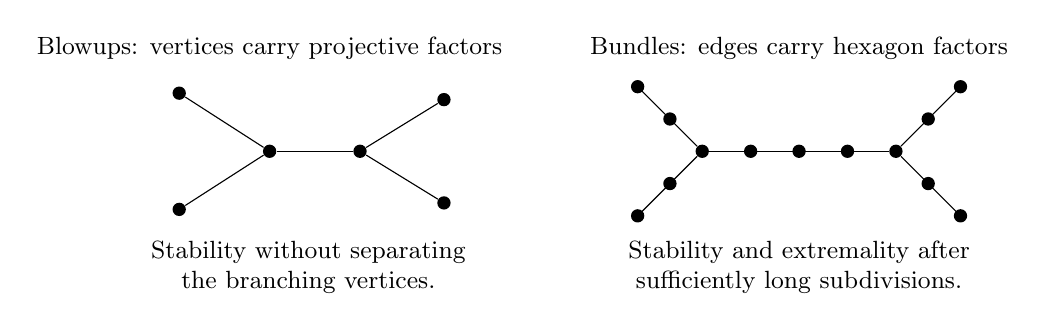
\begin{tikzpicture}[scale=.82,every node/.style={font=\small},
  vertex/.style={circle,fill=black,inner sep=1.7pt}]
\node[align=center] at (0,2.5) {Blowups: vertices carry projective factors};
\node[vertex] (a) at (0,0.9) {};
\foreach \name/\x/\y in {b/-1.4/1.8,c/-1.4/0,d/1.4/0.9}{
 \node[vertex] (\name) at (\x,\y) {}; \draw (a)--(\name);}
\foreach \name/\x/\y in {e/2.7/1.7,f/2.7/0.1}{
 \node[vertex] (\name) at (\x,\y) {}; \draw (d)--(\name);}
\node[align=center,text width=5.7cm] at (.6,-.9)
 {Stability without separating\\
 the branching vertices.};
\begin{scope}[xshift=8.2cm]
\node[align=center] at (0,2.5) {Bundles: edges carry hexagon factors};
\node[vertex] (p) at (-1.5,.9) {};
\node[vertex] (q) at (1.5,.9) {};
\foreach \x in {-.75,0,.75}{\node[vertex] at (\x,.9) {};}
\draw (p)--(q);
\foreach \x/\y in {-2.5/1.9,-2.5/-.1}{
 \draw (p)--(\x,\y);\node[vertex] at (\x,\y) {};
 \node[vertex] at ({(-1.5+\x)/2},{(.9+\y)/2}) {};}
\foreach \x/\y in {2.5/1.9,2.5/-.1}{
 \draw (q)--(\x,\y);\node[vertex] at (\x,\y) {};
 \node[vertex] at ({(1.5+\x)/2},{(.9+\y)/2}) {};}
\node[align=center,text width=5.7cm] at (0,-.9)
 {Stability and extremality after\\
 sufficiently long subdivisions.};
\end{scope}
\end{tikzpicture}
\end{adjustbox}
\caption{Two uses of a subcubic tree. On the left an edge specifies a
codimension-two blowup; on the right it specifies a fibre factor with
opposite twists. The right-hand subdivisions are schematic: the theorem
requires the stated sufficient lengths.}
\label{fig:two-constructions}
\end{figure}


\subsection*{Relation to earlier work and proof structure}
The subspace criterion and its interpretation as cone-volume
concentration are established toric stability theory
\cite{Klyachko1990,HeringNillSuess2022}. Hering--Nill--S\"u\ss{}
determine stability regions for smooth toric surfaces and varieties
of Picard rank two. Dasgupta--Dey--Khan independently treat Picard
rank two and classify the smooth toric Fano fourfolds of Picard rank
three \cite{DasguptaDeyKhan2020}; the Picard-rank-at-most-two
fourfold case is due to Biswas--Dey--Genc--Poddar
\cite{BiswasDeyGencPoddar2021}. Reynolds treats all $124$ smooth toric
Fano fourfolds and their unstable Harder--Narasimhan filtrations
\cite{Reynolds2023}. Devey develops finite matroid tests for
equivariant reflexive sheaves \cite{Devey2022}. We use saturated
subsheaves, as required by the erratum \cite{DasguptaDeyKhan2021}.
The single-edge blowup with dimensions $(1,3)$ is already stable by
\cite[Proposition~5.6.1(2)]{DasguptaDeyKhan2020}.

Our results address families with no bound on the dimension or number
of factors. For blowups, the new steps are the tree reduction, the
exceptional mixed-intersection identity, and uniform estimates that
separate stable from destabilizing arrangements. The estimates use
Efron's monotonicity theorem through
\cite[Theorems~3.2--3.3]{saumardwellner2018}.
For bundles, the relative tangent obstruction uses a divergence
identity related to \cite[Lemma~2.2 and Eq.~(4.4)]{HenkLinke2014}.
Unlike a centred unweighted fibre polytope, its density weighted by
base-slice volumes may have nonzero first moment. This distinction
gives the obstruction. The polarization is the fixed divisor $-K_X$;
results for polarizations near a pulled-back or contracted class
\cite{NapameTipler2024,ClarkeNapameTipler2025} do not give the needed
inequalities. The preceding paper \cite{Wuebben2026} constructs stable
root-twisted bundles with $\rho=n+2$; allowing the number of surface
factors to grow produces the larger extremum and branching families here.

The bundle existence proofs combine exact finite rational inequalities
with the Birkhoff--Hopf contraction theorem
\cite{EvesonNussbaum1995} and induction. The finite calculations are
premises of proofs covering all lengths, not numerical extrapolations.
Their matrices, inequalities and error estimates are printed in the
appendices and reproduced by the ancillary code. The blowup-tree
arguments use uniform identities, integral comparisons and induction,
with explicit polynomial arithmetic. Appendix~\ref{sec:computation}
also records completed classification checks, including the unique
stable eightfold of Picard number eleven.

After the common stability criterion, Sections~\ref{sec:mixed}--\ref{sec:mixed-tree-threshold}
develop the blowup results. Sections~\ref{sec:interactions}--\ref{sec:subdivided}
treat the bundle obstruction, sharpness and abundance. Complete
path, attachment and three-arm calculations, followed by secondary
families and classification data, are in the appendices. Both Picard
maxima concern specified constructions. The unrestricted extremum
remains open and is discussed in Section~\ref{sec:questions}.

\section{Slope stability and symmetries of the rays}\label{sec:stability}

Let $X=X_\Sigma$ be a smooth toric Fano variety of dimension $n$, with
lattice $N$, dual lattice $M$, and primitive ray generators
$u_\rho\in N$ for $\rho\in\mathcal R:=\Sigma(1)$. Write $D_\rho$ for the
corresponding invariant prime divisor, and put
\[
 d_\rho=D_\rho\cdot(-K_X)^{n-1},\qquad
 D=(-K_X)^n=\sum_{\rho\in\mathcal R}d_\rho,\qquad
 \delta_\rho=\frac{n d_\rho}{D}.
\]
Thus $d_\rho>0$, $\delta_\rho>0$, and $\sum_\rho\delta_\rho=n$.
For a torsion-free sheaf $\mathcal E$, its slope is
$\mu(\mathcal E)=c_1(\mathcal E)\cdot(-K_X)^{n-1}/\operatorname{rk}\mathcal E$.
Stability, respectively semistability, means that every nonzero subsheaf
of smaller rank has strictly smaller slope, respectively no larger
slope. In particular, $\mu(T_X)=D/n$.

\begin{lemma}[Toric slope criterion]\label{lem:klyachko}
The tangent bundle $T_X$ is stable, respectively semistable, if and only
if every nonzero proper complex subspace $V\subset N_\CC$ satisfies
\begin{equation}\label{eq:klyachko}
 w(V):=\sum_{\rho:\,u_\rho\in V}\delta_\rho
 <\dim V,\qquad\text{respectively }w(V)\le\dim V.
\end{equation}
It suffices to test subspaces spanned by ray generators.
\end{lemma}

\begin{proof}
This is the criterion of Hering--Nill--S\"u\ss{}
\cite[Proposition 1.2 and Remark 2.6]{HeringNillSuess2022}, obtained from
Klyachko's filtrations \cite{Klyachko1990}. For completeness, the
decreasing filtrations for $T_X$ on $N_\CC$ are
\[
 E^\rho(i)=
 \begin{cases}
 N_\CC,&i\le0,\\
 \CC u_\rho,&i=1,\\
 0,&i\ge2.
 \end{cases}
\]
The saturated equivariant subsheaf $\mathcal E_V$ associated to $V$ has
induced filtrations $V\cap E^\rho(i)$
\cite[Corollary 0.0.2]{DasguptaDeyKhan2021}, rank $\dim V$, and degree
$\sum_{u_\rho\in V}d_\rho$. Both slope stability and semistability can be
tested on these subsheaves
\cite[Proposition 2.3 and Remark 2.4]{HeringNillSuess2022}.
If $V$ contains rays, their span $V'$ contains exactly the same rays and
has dimension at most $\dim V$, so it has at least the same slope.
If $V$ contains no ray, then $w(V)=0<\dim V$.
\end{proof}

For a rational ray-generated subspace $V$, the saturated subsheaf
$\mathcal E_V$ is also the toric foliation whose general leaves are
orbits of the corresponding subtorus. Its first Chern class is
\[
 c_1(\mathcal E_V)=\sum_{u_\rho\in V}D_\rho.
\]
This follows from the same induced filtrations. In particular, a line
containing a single ray has first Chern class $D_\rho$; a line containing
two opposite rays has the sum of the two divisors.

There is an equivalent convex-geometric normalization. Let
\[
 P=\{m\in M_\RR:\langle m,u_\rho\rangle\ge-1
                    \text{ for all }\rho\}
\]
be the anticanonical polytope, with facets $F_\rho$. With lattice volume,
$H^n=n!\operatorname{Vol}(P)$ and
$D_\rho H^{n-1}=(n-1)!\operatorname{Vol}(F_\rho)$, where $H=-K_X$.
The probability measure assigning to $u_\rho$ the mass
\[
 \nu_P(\rho)=\frac{\operatorname{Vol}(\operatorname{conv}(0,F_\rho))}
                  {\operatorname{Vol}(P)}
            =\frac{\delta_\rho}{n}
\]
is the cone-volume measure, written on ray directions. The criterion
is precisely $\nu_P(V)<\dim(V)/n$. This connection with subspace
concentration is established in \cite{HeringNillSuess2022}; our use of
it will be through the explicit divisor degrees of the two constructions.

\begin{lemma}\label{lem:degreerelation}
The divisor degrees satisfy
\[
 \sum_{\rho\in\mathcal R}d_\rho u_\rho=0.
\]
\end{lemma}

\begin{proof}
For $m\in M$, the principal divisor of the character $\chi^m$ is
$\sum_\rho\langle m,u_\rho\rangle D_\rho$. Its intersection with
$(-K_X)^{n-1}$ vanishes. Pairing with all $m\in M$ gives the assertion.
\end{proof}

\subsection{The ray matroid and invariant subspaces}

The \emph{ray matroid} is the linear matroid on $\mathcal R$ whose rank
function is
\[
 r(S)=\dim_\CC\operatorname{span}\{u_\rho:\rho\in S\},
 \qquad S\subseteq\mathcal R.
\]
A circuit is a minimally linearly dependent set of ray generators.
The components of the matroid are the equivalence classes generated by
requiring all members of a circuit to belong to the same class; a ray
in no circuit forms a singleton class. The matroid is \emph{connected}
if it has a single component.

\begin{lemma}\label{lem:raycomponents}
If $C_1,\ldots,C_s$ are the components of the ray matroid and
$V_a=\operatorname{span}\{u_\rho:\rho\in C_a\}$, then
\[
 N_\CC=V_1\oplus\cdots\oplus V_s.
\]
Every direct-sum decomposition of $N_\CC$ in which each ray generator
lies in a summand is obtained by grouping these component subspaces.
In particular, stability of $T_X$ implies connectedness of its ray matroid.
\end{lemma}

\begin{proof}
Choose a basis $B\subset\mathcal R$. For $\rho\notin B$, the ray $u_\rho$
and the basis vectors occurring with nonzero coefficient in its
expansion form a circuit. All those basis vectors therefore belong to
the same component as $\rho$. Consequently $V_a$ is spanned by the
subset $B\cap C_a$ of this basis, proving the direct sum.
Conversely, a circuit cannot meet two summands of any decomposition
containing every ray in a summand: projecting its dependence to either
summand would give a dependence on a proper subset of the circuit.
Thus each component is contained in one summand. Since the rays span
$N_\CC$, each summand is the sum of the component subspaces it contains.

If $s>1$, the equalities $\sum_a w(V_a)=n=\sum_a\dim V_a$ imply
$w(V_a)\ge\dim V_a$ for at least one component, contradicting
Lemma~\ref{lem:klyachko}.
\end{proof}

\begin{proposition}[Symmetry reduction]\label{prop:symmetry}
Let $A$ be any subgroup of the lattice automorphisms preserving
$\Sigma$. Then $T_X$ is stable if and only if its ray matroid is
connected and
\[
 w(V)<\dim V
\]
for every nonzero proper $A$-invariant subspace $V\subset N_\CC$
spanned by ray generators.
\end{proposition}

\begin{proof}
The group $A$ permutes the rays and preserves their divisor degrees,
so $w(aV)=w(V)$ for $a\in A$. Necessity follows from
Lemmas~\ref{lem:klyachko} and~\ref{lem:raycomponents}.
We prove sufficiency by linear algebra.

For any two subspaces $U,V\subseteq N_\CC$, counting the rays in their
union and intersection gives
\begin{equation}\label{eq:weightsupermodular}
 w(U)+w(V)\le w(U+V)+w(U\cap V).
\end{equation}
Let
\[
 \lambda=\max_{0\ne V\subseteq N_\CC}\frac{w(V)}{\dim V}.
\]
The maximum is attained among the finitely many subspaces spanned by
rays, and $\lambda\ge1$ because $w(N_\CC)=n$. If $U,V$ attain this
maximum, then \eqref{eq:weightsupermodular} and the bound
$w(W)\le\lambda\dim W$ imply that $U+V$ also attains it. They also
imply $w(U\cap V)=\lambda\dim(U\cap V)$, including when the
intersection is zero.
Every maximizing subspace is spanned by rays, since $\lambda>0$.
If $\lambda>1$, the sum of all maximizing subspaces is therefore a
nonzero proper maximizing subspace. It is spanned by rays and is
$A$-invariant, contrary to the hypothesis. Thus $\lambda=1$, and
$T_X$ is semistable by Lemma~\ref{lem:klyachko}.

Call a subspace $V$ \emph{tight} if $w(V)=\dim V$. Every nonzero tight
subspace is spanned by rays: replacing it by the span of its rays
would otherwise contradict $w(W)\le\dim W$.
The preceding argument shows that sums and intersections of tight
subspaces are tight. Moreover, if $U$ and $V$ are tight, equality
holds in \eqref{eq:weightsupermodular}. Since all ray weights are
positive, every ray in $U+V$ then lies in $U$ or in $V$.

There are finitely many nonzero tight subspaces. Let
$U_1,\ldots,U_q$ be the minimal ones under inclusion. Distinct $U_i$
have zero intersection, since an intersection is tight. Their sum is
in fact direct. To see this inductively, put $W=U_1+\cdots+U_{k-1}$.
The intersection $U_k\cap W$ is tight, so minimality implies that it
is either zero or all of $U_k$. In the latter case, choose a ray in
$U_k$. Repeated use of the preceding observation about rays in a sum shows that
this ray lies in some $U_i$ with $i<k$, contradicting
$U_i\cap U_k=0$. Thus
\[
 S=U_1\oplus\cdots\oplus U_q
\]
is tight, is spanned by rays, and is $A$-invariant, since $A$ permutes
the minimal nonzero tight subspaces.

If $S\ne N_\CC$, it contradicts the assumed strict inequality on
invariant subspaces. If $S=N_\CC$, every ray belongs to one of the
$U_i$, again by the same observation. Connectedness of the ray
matroid and Lemma~\ref{lem:raycomponents} force $q=1$. Hence
$U_1=N_\CC$ is minimal among nonzero tight subspaces, so there is no
proper nonzero tight subspace. All the inequalities in
Lemma~\ref{lem:klyachko} are therefore strict.
\end{proof}

\section{Blowups of products of projective spaces}\label{sec:mixed}

We first study blowups of products of projective spaces along invariant
codimension-two centres. A simple graph specifies the two factors meeting
each centre. The main result of this section is
Theorem~\ref{mixed:tree}: on a tree, stability against all tangent
subsheaves is equivalent to one divisor-degree inequality at each vertex.
The proof combines a rank formula for the rays with a divergence identity
for the anticanonical polytope. Section~\ref{sec:intrinsic} interprets
the positive terms in that identity as exceptional intersection numbers;
Sections~\ref{sec:mixed-branching}--\ref{sec:mixed-tree-threshold} then
estimate them to obtain uniform stability and local instability theorems.

\subsection{The fan and its primitive collections}

Let $G=(V,E)$ be a finite nonempty simple graph, and write
$k=|V|$, $m=|E|$, and $d_v=\deg_G(v)$. Assign a positive integer $b_v$
to each vertex. In
\[
 N=\bigoplus_{v\in V}\ZZ^{b_v},
\]
let $R_v$ be the $b_v+1$ primitive ray generators of the standard fan of
$\PP^{b_v}$ in its summand. Thus $\sum_{r\in R_v}r=0$. Suppose
$d_v\le b_v+1$, and assign the edges incident to $v$ injectively to rays
$r_{v,e}\in R_v$. For every $e=\{v,w\}$, subdivide the original two-cone
$\langle r_{v,e},r_{w,e}\rangle$ by the ray
\begin{equation}\label{mixed:exceptional-ray}
 s_e=r_{v,e}+r_{w,e}.
\end{equation}
Denote the resulting fan by $\Sigma(G,b)$ and its variety by $Y(G,b)$.
The injectivity condition makes these pairs of original rays disjoint.
All choices of the assignments are related by permutations of the rays
within the projective-space factors and hence give isomorphic fans.

\begin{proposition}\label{mixed:geometry}
The fan $\Sigma(G,b)$ is independent of the order of subdivision and is
smooth and projective. With $n=\sum_v b_v$, one has
\begin{equation}\label{mixed:dimension}
 \dim Y(G,b)=n,\qquad \rho(Y(G,b))=k+m.
\end{equation}
Its primitive collections are precisely
\begin{align}
 \mathcal C_e&=\{r_{v,e},r_{w,e}\},\qquad e=\{v,w\},
 \label{mixed:edge-collection}\\
 \mathcal P_v(J)&=
 \bigl(R_v\setminus\{r_{v,e}:e\in J\}\bigr)
 \cup\{s_e:e\in J\},\qquad J\subseteq E(v),
 \label{mixed:vertex-collection}
\end{align}
where $E(v)$ is the set of edges incident to $v$. Their primitive relations
are
\begin{equation}\label{mixed:primitive-relations}
 r_{v,e}+r_{w,e}=s_e,\qquad
 \sum_{r\in\mathcal P_v(J)}r
   =\sum_{\substack{e=\{v,w\}\in J}}r_{w,e}.
\end{equation}
Every $Y(G,b)$ is weak Fano, and
\begin{equation}\label{mixed:fano}
 Y(G,b)\text{ is Fano}
 \quad\Longleftrightarrow\quad b_v\ge d_v\quad(v\in V).
\end{equation}
If $G$ is connected, $Y(G,b)$ admits no torically locally trivial bundle
presentation with positive-dimensional complete fibre and
positive-dimensional base.
\end{proposition}

\begin{proof}
In an original maximal cone, the subdivision centres that it contains
use disjoint pairs of basis vectors. The subdivisions are therefore
products of subdivisions of two-dimensional orthants. They commute and
remain unimodular. Each remaining original centre persists after the
other subdivisions. Every step is a toric blowup along a smooth invariant
centre, so the resulting fan is projective. It has $n+k+m$ rays, proving
\eqref{mixed:dimension}.

We first describe all its faces. For a subset $A$ of the final rays,
write $B$ for its original rays and $J$ for the edges whose exceptional
rays belong to $A$. Then $A$ spans a cone if and only if
\begin{enumerate}
\item $B$ contains no endpoint pair $\mathcal C_e$;
\item the union of $B$ with both endpoints of every $e\in J$ contains
      no complete set $R_v$.
\end{enumerate}
Indeed, the smallest original cone containing $s_e$ contains both its
endpoints, whereas the original endpoint pair is removed by subdivision.
This proves necessity. For sufficiency, the second condition places the
expanded set in an original product cone. Within that cone, the
subdivisions act on disjoint coordinate pairs, and the first condition
is exactly the condition for the chosen rays to lie in one of the
resulting cones.

The sets in \eqref{mixed:edge-collection} are minimal nonfaces. The
expansion of $\mathcal P_v(J)$ contains $R_v$, and deleting any one member
removes its unique representative of one ray of $R_v$. At any other
vertex, that expansion contains at most one ray, because $G$ is simple;
it cannot contain the full set of at least two rays of that factor.
There is also no original endpoint pair in $\mathcal P_v(J)$. The face
criterion proves its minimality, including when every member is an
exceptional ray. Conversely, a nonface containing no $\mathcal C_e$
expands to a set containing some $R_v$. Choosing one original or
exceptional representative for each ray of $R_v$ produces a subset
$\mathcal P_v(J)$. The list is complete.

The vector identities \eqref{mixed:primitive-relations} follow from
$\sum_{r\in R_v}r=0$. On the right of the second identity there is at
most one ray in each neighbouring factor. No two of these rays form
another centre, since incidence rays are assigned injectively. They
therefore span a cone of the final fan, and their positive sum lies in
its relative interior. These are the primitive relations, of degrees
$1$ and $b_v+1-|J|$, respectively. Batyrev's primitive-collection
criterion for nefness and ampleness
\cite[Theorem~6.4.9]{CoxLittleSchenck2011} proves that $-K$ is nef and
gives \eqref{mixed:fano}. The anticanonical polytope contains the origin
in its interior and is bounded by completeness, so $-K$ is also big.

Finally, the cone complex of a torically locally trivial bundle is the
join of its fibre and base cone complexes. Its rays partition into fibre
rays and one lift of each base ray, and every primitive collection lies
entirely in one part. This follows on the invariant affine charts, where
the fan is the product of the fibre fan and the base cone; the
identifications agree on common faces. In our fan, the primitive
collection $R_v=\mathcal P_v(\varnothing)$ joins all original rays of
one factor. The collections $\mathcal C_e$ join neighbouring factors,
and $\mathcal P_v(\{e\})$ joins $s_e$ to $b_v\ge1$ original rays.
For connected $G$, all rays consequently lie in one equivalence class
generated by membership in a common primitive collection. They admit
no partition into two nonempty parts respecting every primitive
collection. This excludes every bundle presentation of the stated kind,
including alternative choices of fibre and base.
\end{proof}

The last assertion concerns locally trivial toric bundles; it does not
exclude toric morphisms with special fibres or arbitrary non-equivariant
fibrations. Simplicity of $G$ and injectivity of the incidence assignments
are part of the construction. For example, two parallel edges using the
opposite pairs of rays of $\PP^1\times\PP^1$ give the degree-six del Pezzo
surface, which does not satisfy \eqref{mixed:fano} with these vertex
dimensions.

\subsection{Divisor degrees and a divergence identity}

For the remainder of this section assume $b_v\ge d_v$, and put
$Y=Y(G,b)$. Use the normalized degrees of Section~\ref{sec:stability}:
\begin{equation}\label{mixed:normalized-degrees}
 \delta_r=\frac{nD_r\cdot(-K_Y)^{n-1}}{(-K_Y)^n},
 \qquad \sum_r\delta_r=n.
\end{equation}
They are all positive. Set $C_e=\delta_{s_e}$. There is a common value
$A_v$ for the degrees of the unassigned original rays at $v$, and
\begin{equation}\label{mixed:degree-relations}
 \delta_{r_{v,e}}=A_v-C_e,\qquad
 \sum_v(b_v+1)A_v-\sum_eC_e=n.
\end{equation}
To see this, project the relation $\sum_r\delta_r r=0$ of
Lemma~\ref{lem:degreerelation} onto the $v$-th lattice summand. The
coefficient of an assigned ray is $\delta_{r_{v,e}}+C_e$, and that
of an unassigned ray is its degree. The unique relation among $R_v$
has all coefficients equal, proving the first assertion. Summing all
ray degrees gives the second. In particular,
\begin{equation}\label{mixed:degree-positive}
 0<C_e<A_v\qquad(e\in E(v)).
\end{equation}

There are $q_v=b_v+1-d_v\ge1$ unassigned rays at $v$. Choose one as
the negative sum ray and write the others as an integral basis
$r_{v,1},\ldots,r_{v,b_v}$. If $M=\operatorname{Hom}(N,\ZZ)$, the affine
coordinates $a_{v,j}=1+\langle x,r_{v,j}\rangle$ on $M_\RR$ preserve
lattice measure. We write $a_{v,e}$ for the coordinate assigned to the
incidence $(v,e)$. The anticanonical polytope $P$ is
\begin{equation}\label{mixed:polytope}
 a_{v,j}\ge0,\qquad \sum_{j=1}^{b_v}a_{v,j}\le b_v+1,
 \qquad a_{v,e}+a_{w,e}\ge1\quad(e=\{v,w\}).
\end{equation}
Throughout, volumes are lattice volumes without factorial normalization.
If $F_r$ is the facet corresponding to $r$, then
\begin{equation}\label{mixed:facet-ratio}
 (-K_Y)^n=n!\operatorname{vol}(P),\qquad
 \delta_r=\frac{\operatorname{vol}(F_r)}{\operatorname{vol}(P)}.
\end{equation}
The second formula follows from
$D_r\cdot(-K_Y)^{n-1}=(n-1)!\operatorname{vol}(F_r)$.

\begin{lemma}\label{mixed:flux}
For an edge $e=\{v,w\}$, define
\[
 J_{v,e}=\frac{1}{\operatorname{vol}(P)}
     \int_{F_{s_e}}a_{v,e}\,d\operatorname{vol}.
\]
Then
\begin{equation}\label{mixed:flux-identity}
 (b_v+1)A_v=b_v+\sum_{e\in E(v)}J_{v,e},\qquad
 J_{v,e}+J_{w,e}=C_e,
\end{equation}
and $0<J_{v,e}<C_e<A_v$. In particular, $A_v<1$ at every vertex
of degree one, for every positive value of $b_v$.
\end{lemma}

\begin{proof}
Apply the divergence theorem to the vector field equal to $a_v$ in the
$v$-th coordinate block and zero elsewhere. Its divergence is $b_v$.
The coordinate facets have zero flux. The facet
$\sum_j a_{v,j}=b_v+1$ has flux $(b_v+1)$ times its lattice volume,
and the exceptional facet $F_{s_e}$ has flux
$-\int_{F_{s_e}}a_{v,e}\,d\operatorname{vol}$. All remaining facets have
zero flux. For a primitive integral normal, its Euclidean length in
hypersurface measure cancels the reciprocal factor in the unit-normal
flux. Division by $\operatorname{vol}(P)$ proves the first identity.

On $F_{s_e}$ one has $a_{v,e}+a_{w,e}=1$. Its relative interior has
both coordinates strictly between zero and one, since intersection
with either coordinate facet has smaller dimension. This proves the
second identity and the strict bounds on $J_{v,e}$; the remaining bound
is \eqref{mixed:degree-positive}. At a leaf, the first identity gives
$(b_v+1)A_v=b_v+J_{v,e}<b_v+A_v$, hence $A_v<1$.
\end{proof}

\subsection{A cographic rank formula}

Construct a multigraph $H$ with vertices $o$, the vertices $v$ of $G$,
and one vertex $z_e$ for each edge of $G$. Its edges are indexed by the
rays of $\Sigma(G,b)$ as follows:
\begin{itemize}
\item an assigned ray $r_{v,e}$ corresponds to an edge $z_e\to v$;
\item each unassigned original ray at $v$ corresponds to an edge $o\to v$;
\item the exceptional ray $s_e$ corresponds to an edge $o\to z_e$.
\end{itemize}
The orientations specify an incidence matrix and do not affect graph
connectivity. Thus $H$ has $k+m+1$ vertices and $n+k+m$ edges. It is
connected, even if $G$ is disconnected: each $z_e$ joins the root, each
nonisolated $v$ joins some $z_e$, and an isolated $v$ has unassigned
rays joining it to the root.

\begin{proposition}\label{mixed:rank}
For a subset $S$ of the rays, let $H\setminus S$ denote the graph obtained
by deleting its corresponding edges and retaining all vertices. Then
\begin{equation}\label{mixed:rank-formula}
 r(S)=|S|+1-c(H\setminus S),
\end{equation}
where $c$ counts connected components, including isolated vertices.
Consequently the ray matroid is the cographic matroid of $H$: its bases
are exactly the complements of spanning trees of $H$.
\end{proposition}

\begin{proof}
Let $B$ be the signed incidence matrix of $H$, with positive entries at
the heads of oriented edges, and let $R:\QQ^{E(H)}\to N_\QQ$ send each
edge basis vector to its ray. The row at $v$ maps to
$\sum_{r\in R_v}r=0$, and the row at $z_e$ maps to
$s_e-r_{v,e}-r_{w,e}=0$. Thus the row space of $B$ lies in $\ker R$.
Both spaces have dimension $k+m$: the incidence matrix has that rank
because $H$ is connected, and the original rays span $N_\QQ$. Hence
$\ker R=\operatorname{im}B^{\mathsf T}$.

A relation supported on $S$ is therefore $B^{\mathsf T}f$, where $f$
is constant on every component of $H\setminus S$. Modulo the global
constants, these functions have dimension $c(H\setminus S)-1$.
Subtracting this relation dimension from $|S|$ proves
\eqref{mixed:rank-formula}. Rational and complex ranks agree. A subset
of $n$ rays is a basis precisely when its complement is connected;
that complement has $k+m$ edges on $k+m+1$ vertices, so it is a
spanning tree.
\end{proof}

\subsection{The stability criterion for trees}

\begin{theorem}\label{mixed:tree}
Suppose $G$ is a tree with at least one edge and $b_v\ge d_v$ for all
$v$. Then $T_{Y(G,b)}$ is anticanonically stable if and only if
$A_v<1$ for every vertex, and is semistable if and only if $A_v\le1$
for every vertex. Thus it is strictly semistable when $\max_v A_v=1$
and unstable when $\max_v A_v>1$.
\end{theorem}

\begin{proof}
Let $K$ be the tree obtained by subdividing every edge of $G$ at $z_e$,
so $H$ is obtained from $K$ by adjoining the root and its edges. Give
each edge of $H$ its normalized ray degree. There are $q_v$ root edges
of weight $A_v$ at $v$, one root edge of weight $C_e$ at $z_e$, and
the edge $v z_e$ has weight $A_v-C_e$.

For a ray subset $S$, set $E'=E(H)\setminus S$, write $\delta(E')$
for its total weight, and put
\[
 \beta(E')=|E'|-|V(H)|+c(E').
\]
This is the cycle rank, with all vertices retained. By
Proposition~\ref{mixed:rank}, $r(S)=n-\beta(E')$. Since the total
weight is $n$, the slope inequality becomes
\begin{equation}\label{mixed:complement-test}
 \delta(E')>\beta(E')\qquad\text{when }0<r(S)<n,
\end{equation}
with a weak inequality for semistability.

For a nonempty connected vertex set $Q$ of $K$, let $q(Q)$ count all
root edges at its vertices, including multiplicity, and let $W(Q)$ be
the sum of their weights and the weights of all $K$-edges internal to
$Q$. Define
\[
 D(Q)=W(Q)-(q(Q)-1).
\]
For $Q=K$ this is zero, because the cycle rank and total weight of $H$
both equal $n$. For $Q=\{z_e\}$ it is $C_e>0$.

Otherwise the original vertices in $Q$ form a nonempty connected subtree
$I$ of $G$. All exceptional vertices on internal edges of $I$ belong
to $Q$. Let $\partial I$ be the edges with exactly one endpoint in $I$,
write $v(e)$ for that endpoint, and set $t_e=1$ if $z_e\in Q$, and
$t_e=0$ otherwise. Counting the original-ray contributions and then
using \eqref{mixed:flux-identity} gives
\begin{align*}
 W(Q)
 &=\sum_{v\in I}(b_v+1)A_v
   -\sum_{e\in\partial I}(1-t_e)A_{v(e)}
   -\sum_{e\text{ internal to }I}C_e\\
 &=\sum_{v\in I}b_v+\sum_{e\in\partial I}J_{v(e),e}
   -\sum_{e\in\partial I}(1-t_e)A_{v(e)}.
\end{align*}
There are $|I|-1$ internal edges, and
$\sum_{v\in I}d_v=2(|I|-1)+|\partial I|$. Consequently
\[
 q(Q)-1=\sum_{v\in I}b_v-|\partial I|+
                 \sum_{e\in\partial I}t_e,
\]
and hence
\begin{equation}\label{mixed:boundary-deficit}
 D(Q)=\sum_{e\in\partial I}
 \bigl[J_{v(e),e}+(1-t_e)(1-A_{v(e)})\bigr].
\end{equation}
Assume now $A_v\le1$ for every $v$. If $I$ is proper, its boundary is
nonempty, so this sum is strictly positive. If $I$ contains every original
vertex, connectivity forces $Q=K$. Together with the exceptional singleton
case, this proves $D(Q)>0$ for every nonempty proper connected $Q$.

The selected non-root edges of $E'$ form a forest in $K$. Each component
has a connected vertex set $Q$ and contains every $K$-edge internal to
that set, since $K$ is a tree. If it has $h$ selected root edges, counted
with multiplicity, it contributes $\max(h-1,0)$ to $\beta(E')$. This
remains true when several components join the common root: each component
with a root edge adds one connection and its remaining root edges add
cycles. For $h=0$, its contribution to weight minus cycle rank is
nonnegative, and positive if it contains an edge. For $h\ge1$, completing
the missing root edges gives the exact contribution
\begin{equation}\label{mixed:root-completion}
 D(Q)+\sum_{r\text{ a missing root edge at }Q}(1-\delta_r).
\end{equation}
All root degrees are at most one; indeed $C_e<A_v\le1$. Thus every
component contribution is nonnegative, proving the weak inequalities
in \eqref{mixed:complement-test}.

If every $A_v<1$, all root degrees are strictly below one. Contributions
from proper components with root edges are already positive. A full
component $Q=K$ is also positive if a root edge is missing, by
\eqref{mixed:root-completion}; if none is missing, $E'=E(H)$ and
$S=\varnothing$. Components without root edges contribute positively
whenever they contain an edge. The only remaining graph with no positive
contribution is the empty $E'$, which has $r(S)=n$. Both exceptions lie
outside the tested ranks. This proves every strict inequality.

Conversely, an unassigned ray of degree $A_v$ belongs to a rank-one
subspace of weight at least $A_v$. This is a proper subspace because
$n\ge2$. Stability therefore requires $A_v<1$, and semistability
requires $A_v\le1$. These necessity statements, the inequalities just
proved, and Lemma~\ref{lem:klyachko} give all three alternatives.
\end{proof}

The reduction to vertex inequalities uses two different features of the
construction. Proposition~\ref{mixed:rank} describes all tangent subspace
ranks for any simple graph. For trees, the boundary formula
\eqref{mixed:boundary-deficit} expresses the remaining inequalities as
positive sums of vertex and exceptional contributions. In particular,
the scalar criterion is not obtained by disregarding higher-rank
subsheaves. The tree hypothesis is used in this passage from local
degrees to all subspace inequalities.

\begin{corollary}\label{mixed:single-edge}
For every $p,q\ge1$, the blowup of $\PP^p\times\PP^q$ along the invariant
codimension-two subvariety corresponding to a cone generated by one ray
from each factor has anticanonically stable tangent bundle.
\end{corollary}

\begin{proof}
Both vertices of its graph have degree one. Lemma~\ref{mixed:flux}
gives both strict inequalities required by Theorem~\ref{mixed:tree}.
\end{proof}

For $(p,q)=(1,3)$, this recovers
\cite[Proposition~5.6.1(2)]{DasguptaDeyKhan2020}.

\subsection{Stable paths and the largest Picard number}

\begin{theorem}\label{mixed:paths}
Let $G$ be a path with $L\ge1$ edges, endpoint dimensions $p,q\ge1$,
and dimension two at every internal vertex. Then $T_{Y(G,b)}$ is
anticanonically stable, and
\begin{equation}\label{mixed:path-dimension}
 \dim Y(G,b)=2L+p+q-2,\qquad \rho(Y(G,b))=2L+1.
\end{equation}
At each internal vertex its unassigned normalized degree satisfies
$A_v\le24/25$.
\end{theorem}

\begin{proof}
Fix the incidence coordinate $a$ on one side of an edge and integrate
the coordinates of the branch on the other side. Denote its volume by
$\phi(a)$. We shall use the following properties:
\begin{equation}\label{mixed:incoming-bound}
 \phi(a)>0,\qquad \phi(a)=c:=\phi(1)\ (a\ge1),\qquad
 \phi(a)\ge ac\ (0\le a\le1).
\end{equation}
A leaf of dimension $b$ gives
\[
 \phi_b(a)=\frac{(b+\min(a,1))^b}{b!}.
\]
Indeed, translating its assigned coordinate by the lower bound
$\max(0,1-a)$ leaves a simplex of that capacity. Bernoulli's inequality
gives
\[
 \frac{\phi_b(a)}{\phi_b(1)}
 =\left(1-\frac{1-a}{b+1}\right)^b
 \ge1-\frac{b}{b+1}(1-a)\ge a,
\]
so \eqref{mixed:incoming-bound} holds for every endpoint dimension.

At a degree-two vertex, integration of the coordinate assigned to the
parent transforms an incoming function by
\begin{equation}\label{mixed:path-operator}
 g(a)=\int_0^{2+\min(a,1)}
             (2+\min(a,1)-t)\phi(t)\,dt.
\end{equation}
For a positive input constant beyond one, set
$I_0=\int_0^1\phi(t)\,dt$ and $I_1=\int_0^1t\phi(t)\,dt$.
On $0\le a\le1$, the output is $g(a)=g_0+g_1a+g_2a^2$, where
\[
 g_0=2I_0-I_1+c/2,\qquad g_1=I_0+c,\qquad g_2=c/2.
\]
All coefficients are positive, and $g_0-g_2=2I_0-I_1>0$. Hence
\[
 g(a)-ag(1)=(1-a)(g_0-ag_2)\ge0.
\]
The output is constant beyond one. Induction along each branch proves
\eqref{mixed:incoming-bound} for every incoming function, including
branches whose first input is not quadratic.

At an internal vertex let $\phi$ and $\psi$ be the two incoming
functions. The branches have disjoint coordinate blocks, so their
product is the integrand over $a,b\ge0$, $a+b\le3$. For either input
use subscripts to distinguish $c$, $I_0$ and $I_1$. Splitting this
simplex at $a=1$ and $b=1$ gives its full volume $V$ and its unassigned
facet volume $F$ as
\begin{align}
 V={}&I_{0,\phi}I_{0,\psi}
   +c_\psi(2I_{0,\phi}-I_{1,\phi})
   +c_\phi(2I_{0,\psi}-I_{1,\psi})
   +\tfrac12c_\phi c_\psi,\label{mixed:path-volume}\\
 F={}&c_\phi c_\psi+c_\psi I_{0,\phi}+c_\phi I_{0,\psi}.
 \label{mixed:path-facet}
\end{align}
The first term of $V$ is the unit square, the next two are the regions
with just one coordinate at least one, and the last is the remaining
triangle. Eliminating one coordinate from $a+b=3$ gives the lattice
measure in the formula for $F$.

Define
\[
 i_\phi=I_{0,\phi}/c_\phi,\qquad
 h_\phi=(I_{0,\phi}-I_{1,\phi})/c_\phi,
\]
and similarly for $\psi$. From \eqref{mixed:incoming-bound},
$i_\phi\ge1/2$ and $h_\phi\ge1/6$. Equations
\eqref{mixed:path-volume}--\eqref{mixed:path-facet} become
\[
 \frac{F}{c_\phi c_\psi}=1+i_\phi+i_\psi,\qquad
 \frac{V-F}{c_\phi c_\psi}
   =i_\phi i_\psi+h_\phi+h_\psi-\frac12.
\]
Write $i_\phi=1/2+x$, $i_\psi=1/2+y$, $h_\phi=1/6+u$ and
$h_\psi=1/6+v$, with $x,y,u,v\ge0$. Then
\[
 \frac{24V-25F}{c_\phi c_\psi}
   =24xy+11(x+y)+24(u+v)\ge0.
\]
Thus \eqref{mixed:facet-ratio} gives $A_v=F/V\le24/25<1$ at every
internal vertex. Lemma~\ref{mixed:flux} gives $A_v<1$ at both endpoints.
Theorem~\ref{mixed:tree} proves stability, also for $L=1$, when there
is no internal vertex. The dimension and Picard number follow from
Proposition~\ref{mixed:geometry}.
\end{proof}

\begin{corollary}\label{mixed:maximum}
For every $n\ge1$, the largest Picard number among the smooth Fano
$n$-folds $Y(G,b)$ with stable tangent bundle is
\begin{equation}\label{mixed:maximum-value}
 2\left\lfloor\frac n2\right\rfloor+1.
\end{equation}
Here $G$ ranges over the finite nonempty simple graphs with injective
incidence-ray assignments in the construction above.
\end{corollary}

\begin{proof}
If $G$ is disconnected, its fan is the product of the fans for its
connected components. The tangent bundle is a direct sum of at least
two positive-rank bundles; one summand has slope at least the slope of
the whole bundle. Stability therefore forces connectedness. Consequently
$k\le m+1$, whereas the Fano condition gives
\[
 n=\sum_v b_v\ge\sum_v d_v=2m.
\]
It follows that $\rho=k+m\le2m+1\le2\lfloor n/2\rfloor+1$.

For $n=2L\ge2$, take the length-$L$ path with endpoint dimensions
$(1,1)$. For $n=2L+1\ge3$, take endpoint dimensions $(1,2)$ instead.
Theorem~\ref{mixed:paths} gives stability, and
\eqref{mixed:path-dimension} gives equality in \eqref{mixed:maximum-value}.
For $n=1$, the single-vertex graph with dimension one gives $\PP^1$,
whose rank-one tangent bundle is stable and whose Picard number is one.
\end{proof}

This maximum concerns the specified blowups of products of projective
spaces. It is separate from the bundle-class maximum in
Section~\ref{sec:interactions} and does not give an upper bound for
arbitrary smooth toric Fano varieties.

\section{Exceptional intersections and tangent foliations}
\label{sec:intrinsic}

The quantities $J_{v,e}$ in Lemma~\ref{mixed:flux} measure more than
the number of blowups incident to a factor. They are first moments of
exceptional facets, and they can be recovered from ordinary intersection
numbers on the blowup centres. We establish this interpretation without
assuming that the remaining factors are indexed by a tree. It identifies
the tangent subsheaf whose degree is being estimated and gives a
criterion in terms of a specified collection of exceptional contractions.

\subsection{The radial foliation}

Let $B$ be a smooth projective toric variety and let $b\ge2$. Choose a
torus-fixed point $p\in\PP^b$, distinct invariant hyperplanes
$\mathcal H_1,\ldots,\mathcal H_m$ through $p$, where $0\le m\le b$,
and distinct invariant prime divisors $D_1,\ldots,D_m$ on $B$. Let
\[
 \pi:X\longrightarrow\PP^b\times B
\]
be the successive blowup of the strict transforms of
$\mathcal H_i\times D_i$. Assume that $X$ is Fano, and put
\begin{equation}\label{intrinsic:classes}
 n=\dim X,\qquad H=-K_X,\qquad
 f=\operatorname{pr}_1\circ\pi,\qquad
 L=f^*\mathcal O_{\PP^b}(1).
\end{equation}
The pairs of rays defining the centres are disjoint. In every original
smooth cone their subdivisions act on disjoint pairs of basis vectors.
They therefore commute, all the centres remain smooth, and each
exceptional divisor $E_i$ can be contracted while retaining the other
blowups. The centres themselves need not be disjoint.

Projection from $p$ induces a rational map
\[
 X\dashrightarrow\PP^{b-1}\times B.
\]
Let $\mathcal F$ be the saturation in $T_X$ of the tangent directions
to its general fibres. Thus $\mathcal F$ is the birational transform
of the foliation by lines through $p$, with the $B$-coordinate fixed.

\begin{proposition}\label{intrinsic:foliation}
The sheaf $\mathcal F$ is a rank-one toric foliation and
$\mathcal F\simeq\mathcal O_X(L)$. Its normalized slope is
\begin{equation}\label{intrinsic:slope}
 A:=\frac{\mu_H(\mathcal F)}{\mu_H(T_X)}
   =\frac{nLH^{n-1}}{H^n}
   =\left.\frac{d}{dt}\log\operatorname{vol}(H+tL)\right|_{t=0}.
\end{equation}
In particular, $A\ge1$ excludes stability of $T_X$, and $A>1$ gives
a strict rank-one destabilizer.
\end{proposition}

\begin{proof}
Choose basis rays $r_1,\ldots,r_b$ for the hyperplanes through $p$
and put $r_0=-\sum_jr_j$. On the dense torus, the radial foliation
has tangent line $\CC r_0$. Since $b\ge2$, no other ray of the
projective-space factor lies on this line. Rays of $B$ lie in the
other lattice summand, and the new exceptional rays have nonzero
components in both summands. Thus $r_0$ is the only ray on the line.
The induced tangent filtrations from Lemma~\ref{lem:klyachko} give
$c_1(\mathcal F)=D_{r_0}$. The invariant hyperplane opposite $p$
contains none of the blowup centres, so its strict transform has class
$D_{r_0}=L$.

A saturated rank-one subsheaf of a locally free sheaf on a smooth
variety is reflexive: the quotient is torsion-free, and the depth
lemma gives depth at least two in codimension at least two. It is
therefore a line bundle. This proves the sheaf identification; it
does not assert that the foliation is nonsingular everywhere.
The first equality in \eqref{intrinsic:slope} now follows from
$\mu_H(T_X)=H^n/n$. Near the ample class $H$, algebraic volume is
the top intersection number. Differentiating $(H+tL)^n$ proves the
last equality and the slope conclusions.
\end{proof}

The restriction $b\ge2$ is essential. For a $\PP^1$ factor the two
original rays lie on the same line, and both contribute to its tangent
subsheaf. This is why the leaf estimates in Lemma~\ref{mixed:flux}
are kept separate from the present foliation statement.

\subsection{Mixed intersections on the exceptional centres}

Contract only $E_i$, obtaining $\pi_i:X\to Y_i$ with smooth centre
$Z_i$ of dimension $d=n-2$. The centre is the transverse intersection
of the transforms of $\mathcal H_i\times B$ and $\PP^b\times D_i$.
Their normal line bundles on $Z_i$, in this order, will be denoted
$N_{i,A}$ and $N_{i,B}$. Thus
\[
 N_{Z_i/Y_i}=N_{i,A}\oplus N_{i,B},\qquad
 q_i:E_i=\PP_{\rm lines}(N_{i,A}\oplus N_{i,B})\longrightarrow Z_i.
\]
Let $S_{i,0}$ be the section corresponding to the normal direction
$N_{i,B}$, and let $S_{i,1}$ correspond to $N_{i,A}$. The first is
the intersection with the strict transform of $\mathcal H_i\times B$.
Identify the sections with $Z_i$ and set
\begin{equation}\label{intrinsic:polarizations}
 M_{i,0}=H|_{S_{i,0}}=-K_{Z_i}+N_{i,A},\qquad
 M_{i,1}=H|_{S_{i,1}}=-K_{Z_i}+N_{i,B}.
\end{equation}
These are ample classes. The displayed equalities use additive notation
for line bundles. Indeed, if $\xi=c_1(\mathcal O_{\PP_{\rm lines}(N)}(1))$,
then
\[
 E_i|_{E_i}=-\xi,\qquad
 H|_{E_i}=q_i^*(-K_{Y_i}|_{Z_i})+\xi,
\]
while $\xi$ restricts to $-N_{i,B}$ on $S_{i,0}$ and to $-N_{i,A}$
on $S_{i,1}$. Adjunction gives \eqref{intrinsic:polarizations}.

For the next proposition all products of the $M_{i,j}$ are top
intersection numbers on $Z_i$. Define
\begin{equation}\label{intrinsic:Q}
 Q_i=\sum_{k=0}^{n-2}(k+1)M_{i,0}^{n-2-k}M_{i,1}^k,
 \qquad C_i=\frac{nE_iH^{n-1}}{H^n}.
\end{equation}
The order of the two normal directions is part of these data.

\begin{proposition}\label{intrinsic:intersections}
Let $P$ be the anticanonical polytope of $X$ and $F_i$ its facet
corresponding to $E_i$. On $F_i$, let $t$ be the affine coordinate
which is zero and one on the faces corresponding to $S_{i,0}$ and
$S_{i,1}$, respectively. Then
\begin{align}
 J_i:=\frac{1}{\operatorname{vol}(P)}\int_{F_i}t\,d\operatorname{vol}
 &=\frac{Q_i}{H^n},\label{intrinsic:moment}\\
 C_i&=\frac{n}{H^n}\sum_{k=0}^{n-2}
              M_{i,0}^{n-2-k}M_{i,1}^k.\label{intrinsic:exceptional-degree}
\end{align}
Interchanging the sections gives a positive contribution $J_i^{\rm opp}$
with $J_i+J_i^{\rm opp}=C_i$. If $M_{i,1}-M_{i,0}$ is nef, then
$J_i\ge C_i/2$; if $M_{i,0}-M_{i,1}$ is nef, the inequality reverses.
Numerically equal endpoint classes give $J_i=C_i/2$.
\end{proposition}

\begin{proof}
Let $a_i$ and $c_i$ be the affine support coordinates of the two
original rays defining the $i$-th blowup. The exceptional equation is
$a_i+c_i=1$, with $a_i,c_i\ge0$, so $t=a_i$ has the stated endpoints.
The original two rays extend to an integral basis. On the exceptional
facet, an integral tangent vector can therefore increase $a_i$ by one
and decrease $c_i$ by one. Thus its lattice measure disintegrates as
$dt$ times the lattice measure on the centre, without an index factor.

The slice at $t$ is, up to translation, the moment polytope of
\[
 M_{i,t}=(1-t)M_{i,0}+tM_{i,1}.
\]
One way to see this is to restrict the supporting inequalities of
$H|_{E_i}$ along the two sections: their constants interpolate
affinely, giving precisely the supporting inequalities of $M_{i,t}$.
Both endpoints are ample, so the normal fan remains the fan of $Z_i$
along the entire segment. The slice volume is consequently
$M_{i,t}^{n-2}/(n-2)!$. Since $\operatorname{vol}(P)=H^n/n!$,
\begin{equation}\label{intrinsic:beta-integral}
 J_i=\frac{n(n-1)}{H^n}\int_0^1tM_{i,t}^{n-2}\,dt.
\end{equation}
For $d=n-2$, the coefficient of $M_{i,0}^{d-k}M_{i,1}^k$ in the
integral is
\[
 \binom dk\int_0^1t^{k+1}(1-t)^{d-k}\,dt
 =\frac{k+1}{(d+1)(d+2)}.
\]
This proves \eqref{intrinsic:moment}. Integration without $t$ gives
\eqref{intrinsic:exceptional-degree}, also the projective-bundle
formula for $(H|_{E_i})^{n-1}$. Replacing $t$ by $1-t$ replaces the
coefficient $k+1$ by $n-1-k$, so the two contributions sum to $C_i$.
Their positivity follows from ampleness.

Finally, write $I_k=M_{i,0}^{d-k}M_{i,1}^k$. If
$M_{i,1}-M_{i,0}$ is nef, then
\[
 I_{k+1}-I_k
 =M_{i,0}^{d-k-1}M_{i,1}^k(M_{i,1}-M_{i,0})\ge0.
\]
Pairing $k$ with $d-k$ in
$\sum_k(k-d/2)I_k$ proves $J_i-C_i/2\ge0$.
The reverse nef condition and numerical equality are treated identically.
\end{proof}

\begin{theorem}\label{intrinsic:criterion}
For the blowup and foliation in \eqref{intrinsic:classes},
\begin{equation}\label{intrinsic:defect}
 (b+1)A=b+\sum_iJ_i,\qquad
 A-1=\frac{\sum_iQ_i-H^n}{(b+1)H^n}.
\end{equation}
Consequently $\sum_iQ_i\ge H^n$ excludes stability of $T_X$,
and strict inequality makes $\mathcal F$ a strict destabilizer.
Equivalently, the total contribution is
\begin{align}
 \sum_iJ_i
 &=n\frac{f^*(-K_{\PP^b})H^{n-1}}{H^n}-b\notag\\
 &=(n-b)-n\frac{(-K_{X/\PP^b})H^{n-1}}{H^n}.
 \label{intrinsic:relative-defect}
\end{align}
Here $-K_{X/\PP^b}=H-f^*(-K_{\PP^b})$ denotes the relative
anticanonical divisor class.
\end{theorem}

\begin{proof}
In central affine coordinates the anticanonical polytope has inequalities
\[
 a_j\ge0,\qquad \sum_{j=1}^ba_j\le b+1,\qquad
 a_i+c_i\ge1\quad(1\le i\le m),
\]
together with the inequalities from the rays of $B$. Apply divergence
to $\sum_ja_j\partial/\partial a_j$, whose divergence is $b$.
The coordinate facets and the facets from $B$ have zero flux. The
opposite central facet contributes $(b+1)$ times its lattice volume,
and $F_i$ contributes $-\int_{F_i}a_i$. As in
Lemma~\ref{mixed:flux}, the conversion between Euclidean and lattice
facet measures cancels the normal-length factor. Division by
$\operatorname{vol}(P)$ gives the first identity in
\eqref{intrinsic:defect}. Proposition~\ref{intrinsic:intersections}
gives the second, and Proposition~\ref{intrinsic:foliation} gives the
slope conclusions. Substituting $f^*(-K_{\PP^b})=(b+1)L$ proves
\eqref{intrinsic:relative-defect}.
\end{proof}

Thus an exceptional divisor contributes its normalized degree $C_i$
multiplied by the mean of $t$ in its slice-volume distribution.
The two section polarizations determine how this degree is divided.
For example, the geometric hypotheses $M_{i,1}-M_{i,0}$ nef for every
$i$ and $\sum_iC_i\ge2$ imply failure of stability; a strict weighted
inequality implies instability. We do not impose these nef hypotheses
in the tree theorems below. The identity, which does not require them,
retains the effect of all other blowups through $Z_i$ and $M_{i,0},M_{i,1}$.
It also distinguishes an individual foliation test from a test of every
subsheaf: $\sum_iQ_i<H^n$ controls $\mathcal F$ alone.

\subsection{Geometric slice profiles}

There is a second useful description when $m=b$ and
$B=\prod_{i=1}^bB_i$, with $D_i$ pulled back from a smooth invariant
prime divisor on $B_i$. Put $d_i=\dim B_i$ and $h_i=-K_{B_i}$.
Assume that $h_i$ and $h_i-D_i$ are ample, as well as $H=-K_X$.
Define the positive continuous functions
\begin{equation}\label{intrinsic:profiles}
 p_i(a)=
 \begin{cases}
 (h_i-(1-a)D_i)^{d_i}/d_i!,&0\le a\le1,\\
 h_i^{d_i}/d_i!,&a\ge1.
 \end{cases}
\end{equation}
These functions express the volume of a divisor segment on the base.

\begin{proposition}\label{intrinsic:profile-test}
In this product-base setting, let
\[
 Z(t)=\int_{\substack{a_i\ge0\\\sum_i a_i\le t}}
                 \prod_i p_i(a_i)\,da_1\cdots da_b.
\]
Then
\begin{equation}\label{intrinsic:profile-slope}
 A=\frac{Z'(b+1)}{Z(b+1)},\qquad
 \frac{p_i'(a)}{p_i(a)}
 =\frac{d_iD_i(h_i-(1-a)D_i)^{d_i-1}}
        {(h_i-(1-a)D_i)^{d_i}}\quad(0<a<1).
\end{equation}
If $q_i$ are positive continuous log-concave functions, constant beyond
one, and every $p_i/q_i$ is nonincreasing, then $A$ is at most the
corresponding ratio $Z_q'(b+1)/Z_q(b+1)$. Nondecreasing ratios give
the reverse inequality.
\end{proposition}

\begin{proof}
At fixed $a_i\in[0,1]$, the exceptional constraint moves the facet of
$D_i$ inward by $1-a_i$. The remaining polytope is therefore the
moment polytope of $h_i-(1-a_i)D_i$. The ample endpoint assumption
keeps the whole segment in the same ample cone and gives exactly
\eqref{intrinsic:profiles}. For $a_i\ge1$ the new constraint is
redundant. Independence of the base factors gives the product
integrand. Hence $Z(b+1)$ is the full polytope volume, and $Z'(b+1)$
is the lattice volume of the opposite central facet. Their ratio is
$A$. Differentiating the intersection polynomial gives the second
formula in \eqref{intrinsic:profile-slope}. The comparison is
Lemma~\ref{treemix:convolution}, proved below from Efron's
conditional-sum theorem; it requires log-concavity of the reference
profiles only.
\end{proof}

For a vertex $v$ of a blowup tree, deleting $v$ separates the remaining
construction into factors $B_i$. The divisor at the former parent
incidence becomes an unassigned divisor $D_i$ on its component.
Its class is the pullback of a hyperplane at that component's root.
The classes $h_i-D_i$ are ample: after deleting the parent edge,
every primitive relation of root type has degree at least two.
Subtracting $D_i$ lowers each such degree by one, while edge and
non-root primitive relations are unchanged.
Thus the incoming functions in the tree calculations are precisely the
intersection polynomials \eqref{intrinsic:profiles}.

The proof of Theorem~\ref{treemix:subcubic} bounds their logarithmic
derivatives above by $3/(2+a)$ when every nonleaf dimension equals its
valence and the maximum degree is three. The degree-four obstruction
instead supplies four profiles bounded below in ratio order by
\eqref{treemix:g-four}. Proposition~\ref{intrinsic:profile-test}
allows either comparison to be tested on other polarized base pairs,
without assigning a construction graph to those factors. Outside the
tree criterion, an upper bound concerns only the radial foliation;
a lower bound exceeding one still proves instability of $T_X$.

Neither this description nor \eqref{intrinsic:relative-defect} asserts
that a large Picard number forces the required contraction data or
intersection inequality. That is a separate structural problem. Also,
the edges of the bundle constructions in Section~\ref{sec:graphs}
represent twists, not the exceptional divisors used here; their
subdivision theorems do not assert monotonicity of these blowup weights.

\section{Branching and neighbouring factor dimensions}\label{sec:mixed-branching}

We retain the mixed-blowup construction $Y(G,b)$ of
Section~\ref{sec:mixed}, with distinct original rays assigned to the
incidences at each vertex. Write $d_v=\deg_G(v)$. Throughout this
section assume $b_v\ge d_v$ and $b_v\ge1$ at every vertex, so that
$Y(G,b)$ is Fano. A vertex $v$ is
\emph{saturated} if $b_v=d_v$; equivalently, exactly one of its original
rays is unassigned. The degree of its unassigned divisor depends on
the geometry beyond its incident centres. We first determine stability
for saturated stars, including the stable degree-four and degree-five
examples. We then show that replacing the rest of the geometry by
independent leaves of the same neighbouring dimensions can only decrease
this degree. This comparison allows cycles and does not require
saturation at the other vertices.

\subsection{The exact transition for stars}

Let $Y_m$ be the mixed blowup associated with a star with $m\ge1$ edges,
central dimension $m$, and dimension one at each leaf. In the product
lattice, choose bases $e_1,\ldots,e_m$ for the central factor and $u_i$
for leaf $i$. Put
\[
 e_0=-\sum_{i=1}^m e_i,\qquad s_i=e_i+u_i.
\]
Thus $Y_m$ is obtained from $\PP^m\times(\PP^1)^m$ by subdividing the
$m$ original cones $\langle e_i,u_i\rangle$. Let $A_m$ denote the
normalized divisor degree of $e_0$, with the normalization used in
Section~\ref{sec:mixed}.

\begin{theorem}\label{branch:stars}
For every $m\ge1$, the variety $Y_m$ is smooth Fano, has dimension $2m$
and Picard number $2m+1$, and admits no torus-equivariantly locally
trivial bundle presentation with positive-dimensional complete fibre
and positive-dimensional base. Its tangent bundle is anticanonically
stable exactly when $1\le m\le5$. For every $m\ge6$, the line
$\CC e_0$ defines a strictly destabilizing saturated subsheaf.
\end{theorem}

The proof, including the finite sign calculation and the uniform tail
estimate, is given in Appendix~\ref{sec:blowup-comparisons}.


For the two stable stars with higher valence, the central degrees and
total exceptional contributions are
\[
 A_4=\frac{44080}{47119},\qquad
 \sum_iJ_{0,i}=\frac{31924}{47119}<1;
 \qquad
 A_5=\frac{100780}{103289},\qquad
 \sum_iJ_{0,i}=\frac{88235}{103289}<1.
\]
These values follow from the table and \eqref{mixed:flux-identity}.
They show that neither four nor five incident blowups alone forces the
radial foliation of Proposition~\ref{intrinsic:foliation} to destabilize.
The neighbouring slice profiles, rather than the number of contributions,
determine whether their sum reaches one.

The same line is the first Harder--Narasimhan term for $m\ge6$
(Corollary~\ref{branch:hn}).

\subsection{Comparison at a saturated vertex}

The star calculation gives a necessary condition for stability in the
entire simple-graph construction. In the next statement, the graph need
not be connected and may contain cycles.

\begin{theorem}\label{branch:comparison}
Let $G$ be a finite simple graph with positive dimensions $b_w\ge d_w$
at every vertex, and use injective incidence assignments in the
construction of $Y(G,b)$. Suppose $v$ is saturated and
$b_v=d_v=m\ge1$. Let $A_v$ be the normalized divisor degree of its unique
unassigned original ray. Enumerate the neighbors as $w_1,\ldots,w_m$
and put $c_i=b_{w_i}$. Define
\[
 \phi_c(a)=\frac{(c+\min(a,1))^c}{c!},\qquad
 Z_{\mathbf c}(t)=\int_{\substack{a_i\ge0\\\sum_i a_i\le t}}
                  \prod_{i=1}^m\phi_{c_i}(a_i)\,da.
\]
Then
\[
 A_v\ge\frac{Z'_{\mathbf c}(m+1)}{Z_{\mathbf c}(m+1)}
       \ge A_m.
\]
The first ratio is nondecreasing in each neighboring dimension $c_i$.
The dimensions at vertices other than $v$ may exceed their degrees.
\end{theorem}

\begin{proof}
At every vertex $w$, choose an unassigned original ray as the negative
sum ray, and use the other $b_w$ rays as a lattice basis. This is
possible because $b_w\ge d_w$. In affine coordinates
$a_{w,j}=1+\langle x,r_{w,j}\rangle$, the anticanonical polytope is
\begin{equation}\label{branch:graph-polytope}
 a_{w,j}\ge0,\qquad
 \sum_{j=1}^{b_w}a_{w,j}\le b_w+1,\qquad
 a_{w,e}+a_{z,e}\ge1\quad(e=\{w,z\}).
\end{equation}
Here $a_{w,e}$ is the coordinate assigned to the incidence $(w,e)$.
The coordinate change preserves lattice volume.

Write $a=(a_1,\ldots,a_m)$ for the coordinates at $v$. Before imposing
the simplex inequality at $v$, integrate over all other vertices and
denote the resulting volume by $W(a)$, for every $a_i\ge0$.
It is bounded by the product of the other simplex volumes and is
coordinatewise nondecreasing, since increasing $a_i$ only relaxes one
inequality. It is constant in each coordinate once that coordinate is
at least one.

Moreover, $W(0)>0$. At every other vertex choose its assigned
coordinates equal to $1+\varepsilon$ and its remaining coordinates
equal to $\varepsilon$. For sufficiently small $\varepsilon>0$, the
sum at $w$ is $d_w+b_w\varepsilon<b_w+1$, and all mixed inequalities
are strict. An open set of such choices has positive volume.
Monotonicity gives $W(a)>0$ throughout the nonnegative orthant.
The function $W$ is continuous: its domain is contained in a fixed
compact product of simplexes, and under a convergent change of $a$
the defining indicators converge away from finitely many affine
hyperplanes of measure zero.

We first prove that
\begin{equation}\label{branch:ratio}
 R(a)=\frac{W(a)}{\prod_{i=1}^m\phi_{c_i}(a_i)}
\end{equation}
is coordinatewise nondecreasing. Fix every central coordinate except
$a_i$, and let $w$ be the other endpoint of its edge. Put $b=b_w$.
At $w$, let $x$ be the coordinate assigned to this edge and let
$z=(z_1,\ldots,z_{b-1})$ be its remaining coordinates. Injectivity of
the incidence assignments ensures that no other mixed inequality
uses $x$. Simplicity ensures that $w$ has no second edge to $v$.

Temporarily omit the simplex inequality at $w$ and integrate over
every vertex other than $v,w$. The resulting function $\Psi(z)$ is
nonnegative and coordinatewise nondecreasing on the nonnegative
orthant: increasing a component of $z$ only enlarges the feasible set.
It may depend on the other fixed central coordinates, but it is
independent of $x$ and $a_i$. Edges among the other vertices remain
inside this integral, so no independence of neighbouring components
is required.

For $0\le a_i\le1$, the interval for $x$ is
$[1-a_i,b+1-\sum_jz_j]$. With $s=b+a_i$, integration over this interval
and then the substitution $z=sy$ give
\begin{align}
 W(a)
 &=\int_{\substack{z_j\ge0\\\sum_jz_j\le s}}
       (s-\textstyle\sum_jz_j)\Psi(z)\,dz \notag\\
 &=s^b\int_{\substack{y_j\ge0\\\sum_jy_j\le1}}
       (1-\textstyle\sum_jy_j)\Psi(sy)\,dy.
 \label{branch:neighbour-integral}
\end{align}
When $b=1$, the last integral is zero-dimensional and the same identity
holds. The integral factor is nondecreasing in $s$. Thus, with the
other coordinates fixed and $0\le a\le a'\le1$,
\[
 \frac{W(a')}{W(a)}
 \ge\left(\frac{b+a'}{b+a}\right)^b
 =\frac{\phi_b(a')}{\phi_b(a)}.
\]
This proves monotonicity
of $R$ below one in each coordinate. Above one both $W$ and $\phi_{c_i}$
are constant, and continuity gives the assertion across one.
The function $R$ is also bounded, since each $\phi_{c_i}$ has a positive lower bound.

To compare the simplex integrals, introduce independent random variables
$X_1,\ldots,X_m$ with respective densities
\[
 f_i(x)=C_i e^{-x}\phi_{c_i}(x)\mathbf 1_{\{x\ge0\}},
\]
where $C_i>0$ is the normalizing constant. Each density is log-concave.
On $(0,1)$ its logarithmic derivative is $-1+c_i/(c_i+x)$, which decreases;
at one this derivative jumps downward to $-1$ and stays constant
thereafter. Its support is the interval $[0,\infty)$.

Efron's conditional-sum theorem states that, for independent
log-concave random variables, the conditional expectation of a bounded
coordinatewise nondecreasing function is nondecreasing in their sum;
the version for general log-concave densities and any finite number
of variables is given in
\cite[Theorems~3.2--3.3]{saumardwellner2018}.
Extend $R$ to $\RR^m$ by replacing each argument by its nonnegative
part. The extension is bounded and coordinatewise nondecreasing.
The theorem therefore implies that
\[
 h(s)=\mathbb E\!\left[
 R(X_1,\ldots,X_m)\,\middle|\,X_1+\cdots+X_m=s
 \right]
\]
has a nondecreasing version. When $m=1$, the same assertion follows
directly from $h(s)=R(s)$.

On the slice $\sum_i a_i=s$, the product exponential factor equals
$e^{-s}$ and cancels from the conditional expectation. Thus $h(s)$
is the ratio of the $W$-weighted slice volume to the
$\prod_i\phi_{c_i}(a_i)$-weighted slice volume. These integrals are
continuous for $s>0$, by rescaling the compact sum simplex to a fixed
simplex and applying dominated convergence. The denominator is
positive. Their ratio consequently agrees everywhere on $(0,\infty)$
with the nondecreasing version supplied by the theorem.

Set
\[
 F(t)=\int_{\substack{a_i\ge0\\\sum_i a_i\le t}}W(a)\,da,
 \qquad q(t)=Z'_{\mathbf c}(t)>0.
\]
Using the lattice slice measure obtained by eliminating one coordinate,
we have
\[
 F'(t)=q(t)h(t),\qquad
 F(t)=\int_0^tq(s)h(s)\,ds
 \le h(t)Z_{\mathbf c}(t).
\]
All quantities are positive, so
\[
 \frac{F'(t)}{F(t)}\ge\frac{Z'_{\mathbf c}(t)}{Z_{\mathbf c}(t)}.
\]
At $t=m+1$, the denominator on the left is the full anticanonical
polytope volume and its numerator is the lattice volume of the
unassigned facet at $v$. Their ratio is $A_v$, proving the first comparison.

For integers $b\ge c\ge1$ and $0<a<1$,
\[
 \frac{d}{da}\log\frac{\phi_b(a)}{\phi_c(a)}
 =\frac{a(b-c)}{(b+a)(c+a)}\ge0.
\]
The ratio is constant above one. Applying the same conditional-sum
argument to products of these ratios proves monotonicity in the
neighboring dimensions. Taking every $c_i=1$ gives
$\phi_1(a)=1+\min(a,1)$ and recovers the star ratio, proving the
second comparison.
\end{proof}

\begin{corollary}\label{branch:obstruction}
In the Fano simple-graph mixed-blowup construction, a saturated vertex of
degree at least six forces anticanonical tangent instability. In
particular, if every vertex is saturated and the tangent bundle is
stable, then the maximum graph degree is at most five. The star $Y_5$
attains degree five.
\end{corollary}

\begin{proof}
Let $v$ be saturated of degree $m\ge6$. Theorems~\ref{branch:stars}
and~\ref{branch:comparison} give $A_v\ge A_m>1$. Its unassigned ray
is the negative sum of $m$ basis vectors and is not collinear with
another original ray in that factor. Original rays at other vertices
lie in different direct summands, and exceptional rays have nonzero
components in two summands. Thus its line has normalized ray weight
exactly $A_v>1$ and defines a strict rank-one destabilizer.
The last assertion follows from Theorem~\ref{branch:stars}.
\end{proof}

\begin{corollary}\label{branch:degree-five}
If a saturated degree-five vertex has at least four neighbors of factor
dimension at least two, its unassigned divisor degree satisfies
\[
 A_v\ge\frac{6244655501}{6233518181}>1,
\]
and its unassigned ray defines a strict rank-one destabilizer.
Consequently, in a saturated simple graph with stable tangent bundle,
each degree-five vertex has at least two degree-one neighbors.
\end{corollary}

\begin{proof}
Theorem~\ref{branch:comparison} reduces the assertion to the neighboring
dimensions $(2,2,2,2,1)$. Their simplex and facet volumes at capacity six are
\[
 Z(6)=\frac{6233518181}{362880},\qquad
 Z'(6)=\frac{892093643}{51840}.
\]
To specify these rational calculations explicitly, let $c_{j,k}$ be
the coefficient of $q^ju^k$ in
\[
 (2u^2+2u+1-q(3u+1))^4(u+1-q).
\]
The Laplace transforms of $\phi_1,\phi_2$ are respectively
$(s+1-e^{-s})/s^2$ and
$(2s^2+2s+1-e^{-s}(3s+1))/s^3$. Thus
\[
 Z(6)=\sum_{j,k}c_{j,k}\frac{(6-j)^{14-k}}{(14-k)!},\qquad
 Z'(6)=\sum_{j,k}c_{j,k}\frac{(6-j)^{13-k}}{(13-k)!},
\]
where $0\le j\le5$ and $0\le k\le9$. These finite sums give the displayed
values. The unassigned ray is the only ray on its line, by the same
direct-summand argument as in Corollary~\ref{branch:obstruction}.
Its weight exceeds one, so the line strictly destabilizes.
In the saturated case neighboring dimensions equal neighboring degrees;
at most three of the five neighbors can therefore have degree at least two.
\end{proof}

\begin{corollary}\label{branch:subdivision}
A saturated five-arm tree is unstable whenever at least four of its arms
have length at least two. In particular, subdivision of four arms of the
stable five-arm star produces an unstable mixed blowup, and further
subdivision of those arms preserves this obstruction.
\end{corollary}

\begin{proof}
The central vertex has degree five and at least four degree-two neighbors,
so Corollary~\ref{branch:degree-five} applies.
\end{proof}

Here subdivision refers to the indexing graph: its factor dimensions
and the dimension of the variety change. It is not a fan subdivision in
fixed dimension. The obstruction rules out a general stability theorem
obtained merely by making every arm of a mixed-blowup tree sufficiently
long. It concerns saturated vertices and places no corresponding degree
bound on vertices whose dimensions exceed their degrees.

\section{A sharp universal degree threshold for blowup trees}
\label{sec:mixed-tree-threshold}

We now prove that every tree of maximum degree three gives a stable
blowup when the nonleaf dimensions equal their valences; the leaf
dimensions can be arbitrary. The argument controls the incoming volume
profiles uniformly under both the one-child and two-child integration
operations. Four neighbours with sufficiently large profiles instead
force the central radial foliation to destabilize. This yields a sharp
universal degree threshold, while allowing the stable degree-four and
degree-five arrangements of Section~\ref{sec:mixed-branching}.
A family with two branching vertices gives further stable arrangements.

\begin{theorem}\label{treemix:subcubic}
Let $G$ be a finite tree with at least one edge and maximum degree at
most three. Set $b_v=d_v$ at every nonleaf vertex, and choose any positive
integer $b_v$ at each leaf. Then the mixed blowup $Y(G,b)$ has
anticanonically stable tangent bundle. If $M=|E(G)|$, then
\[
 n=2M+\sum_{v\text{ leaf}}(b_v-1),\qquad \rho=2M+1.
\]
It is smooth Fano and admits no torus-equivariantly locally trivial
bundle presentation with positive-dimensional complete fibre and base.
The normalized degrees of unassigned original divisors satisfy
\begin{equation}\label{treemix:local-bounds}
 A_v\le\frac{25950132}{26414113}<1\quad(d_v=3),\qquad
 A_v\le\frac{24}{25}<1\quad(d_v=2).
\end{equation}
In particular, every saturated tree of maximum degree three gives such
a stable variety with $n=2M$ and $\rho=n+1$.
\end{theorem}

There is no restriction on the distances between branching vertices or
on the relative sizes of the components of $G-v$. The numerical bounds
in \eqref{treemix:local-bounds} concern the indicated individual divisor
degrees; they do not give a uniform slope gap for all proper subspaces
or for leaves of arbitrary dimension.

In the notation of Section~\ref{sec:intrinsic}, the two internal-vertex
bounds imply
\[
 \sum_{e\ni v}J_{v,e}\le\frac{24558189}{26414113}<1
 \quad(d_v=3),\qquad
 \sum_{e\ni v}J_{v,e}\le\frac{22}{25}<1
 \quad(d_v=2).
\]
The proof therefore bounds the sum of the ordered exceptional
intersections, including their dependence on all farther branches.
Theorem~\ref{mixed:tree} is the additional step that promotes these
local inequalities to stability of the entire tangent bundle.

\subsection{Comparison of simplex integrals}

We use two elementary integral constructions together with Efron's
conditional-sum theorem. A function in this subsection is positive and
continuous on $[0,\infty)$ and constant on $[1,\infty)$. For $k\ge1$ set
\[
 V_{p_1,\ldots,p_k}(t)=
 \int_{\substack{x_i\ge0\\\sum_i x_i\le t}}\prod_i p_i(x_i)\,dx,
 \qquad F_{p_1,\ldots,p_k}(t)=V'_{p_1,\ldots,p_k}(t),
\]
and
\[
 B_{p_1,\ldots,p_k}(t)=
 \int_{\substack{x_i\ge0\\\sum_i x_i\le t}}
       (t-\textstyle\sum_i x_i)\prod_i p_i(x_i)\,dx.
\]
The derivative $F$ is the integral on the sum slice in lattice measure,
obtained by eliminating one coordinate with coefficient one.

\begin{lemma}\label{treemix:convolution}
Let $p_i,q_i$ be functions as above, with $q_i$ log-concave. If every
$p_i/q_i$ is nonincreasing, then
\[
 \frac{B_{p_1,\ldots,p_k}(t)}{B_{q_1,\ldots,q_k}(t)}
 \quad\hbox{and}\quad
 \frac{F_{p_1,\ldots,p_k}(t)}{F_{q_1,\ldots,q_k}(t)}
\]
are nonincreasing for $t>0$, and
\begin{equation}\label{treemix:root-comparison}
 \frac{F_{p_1,\ldots,p_k}(t)}{V_{p_1,\ldots,p_k}(t)}
 \le\frac{F_{q_1,\ldots,q_k}(t)}{V_{q_1,\ldots,q_k}(t)}.
\end{equation}
If every $p_i/q_i$ is nondecreasing, both monotonicity assertions and
inequality \eqref{treemix:root-comparison} reverse.
\end{lemma}

\begin{proof}
Take independent variables $X_i$ with densities proportional to
$e^{-x}q_i(x)$ on $[0,\infty)$, and two further independent exponential
variables of rate one. These densities are log-concave. The bounded
positive function $R(x)=\prod_i p_i(x_i)/q_i(x_i)$ has the asserted
coordinatewise monotonicity and is independent of the two extra
coordinates. Extend it to real arguments by their nonnegative parts.
Efron's conditional-sum theorem
\cite[Theorems~3.2--3.3]{saumardwellner2018} makes its conditional
expectation monotone in the total sum. The nonincreasing version follows
by applying the theorem to $-R$.

On a slice of total $t$, the common exponential factor cancels. Integrating
the two additional coordinates gives the factor $t-\sum_i x_i$, so the
conditional expectation is exactly $B_p(t)/B_q(t)$. Omitting these two
variables instead gives $h(t)=F_p(t)/F_q(t)$; for $k=1$ this is just the
assumed ratio order. Rescaling to a fixed compact simplex proves continuity
of all slice ratios for $t>0$. Their positive denominators ensure that
the monotone versions supplied by the theorem agree with these ratios
everywhere. In the nonincreasing case,
\[
 V_p(t)=\int_0^t F_q(s)h(s)\,ds\ge h(t)V_q(t),\qquad
 F_p(t)=F_q(t)h(t).
\]
Division proves \eqref{treemix:root-comparison}. The same calculation
with the reversed integral inequality proves the other case.
\end{proof}

The following coefficient identity specifies the finite rational
calculations used below. For a function $p$ as above define the formal
power series
\begin{equation}\label{treemix:Q}
 Q_p(z)=p(1)+z\sum_{j\ge0}\frac{z^j}{j!}
                   \int_0^1(1-a)^jp(a)\,da.
\end{equation}
Only finitely many coefficients are needed in each application.

\begin{lemma}\label{treemix:coefficients}
For $k\ge1$, $r\ge0$, and an integer $s\ge0$,
\begin{equation}\label{treemix:split}
 \int_{\substack{a_i\ge0\\\sum_i a_i\le k+r}}
 \frac{(k+r-\sum_i a_i)^s}{s!}\prod_i p_i(a_i)\,da
 =[z^{k+s}]e^{rz}\prod_i Q_{p_i}(z).
\end{equation}
For $r>0$, the facet volume is
\[
 F_{p_1,\ldots,p_k}(k+r)=[z^{k-1}]e^{rz}\prod_i Q_{p_i}(z).
\]
\end{lemma}

\begin{proof}
Partition the domain according to the set $S$ of coordinates in $[0,1]$.
Subtract one from each of the remaining $k-|S|$ coordinates. Their
integration leaves
\[
 \frac{(r+\sum_{i\in S}(1-a_i))^{k-|S|+s}}{(k-|S|+s)!}
 \prod_{i\notin S}p_i(1)
\]
times the product of the short-coordinate weights. Express this power
as an exponential coefficient, integrate the short coordinates over
$[0,1]^S$, and sum over $S$. The result is
\eqref{treemix:split}. Differentiate the case $s=0$ with respect to $r$
to obtain the facet formula.
\end{proof}

\subsection{The proof for maximum degree three}

Fix an oriented edge towards a parent vertex. With the parent's
incidence coordinate equal to $a$, integrate over the component on
the other side of the edge and denote its volume by $p(a)$.
These incoming functions are positive, continuous, and constant for
$a\ge1$. Indeed, the only inequality involving the fixed coordinate is
$a+x\ge1$; above one it is redundant. Positivity follows by choosing
all assigned coordinates slightly greater than one and all remaining
coordinates small and positive. The inequalities $b_v\ge d_v$ leave
room in every vertex simplex. Continuity follows by dominated convergence
inside the fixed compact product of these simplexes. Since removing a
vertex separates the tree into disjoint components, the incoming
functions multiply when its coordinates are fixed.

For a leaf of dimension $b$, the incoming function is
\[
 \phi_b(a)=\frac{(b+\min(a,1))^b}{b!}.
\]
At a nonleaf of degree two or three, integration of the coordinate
assigned to the parent gives, for $0\le a\le1$,
\begin{align}
 T(p)(a)&=B_p(2+a),\label{treemix:T}\\
 \mathcal G(p,q)(a)&=B_{p,q}(3+a),\label{treemix:G}
\end{align}
followed by constant continuation. There are respectively one and two
child coordinates; the remaining interval has length
$2+a-x$ or $3+a-x-y$.

\begin{proof}[Proof of Theorem~\ref{treemix:subcubic}]
Put $P(a)=(2+\min(a,1))^3$, and write $p\preceq P$ if $p/P$ is
nonincreasing. The reference $P$ is an auxiliary function, not the
volume of an additional projective-space factor. It is log-concave:
its logarithmic derivative is $3/(2+a)$ below one and drops to zero
above one. Every leaf satisfies $\phi_b\preceq P$, since
\[
 \frac{d}{da}\log\frac{\phi_b(a)}{P(a)}
 =\frac b{b+a}-\frac3{2+a}\le1-\frac3{2+a}\le0
 \qquad(0<a<1).
\]
This includes every positive leaf dimension.

We next prove closure under \eqref{treemix:T}--\eqref{treemix:G}.
Direct integration, or Lemma~\ref{treemix:coefficients}, gives
\begin{align*}
 T(P)(a)&=\frac{363}{10}+\frac{173}{4}a+\frac{27}{2}a^2,\\
 \mathcal G(P,P)(a)&=\frac{119659}{80}+\frac{148781}{80}a
                  +\frac{3213}{4}a^2+\frac{243}{2}a^3.
\end{align*}
For a polynomial $g$ of degree at most three,
\[
 \left(\frac{g(a)}{(2+a)^3}\right)'
 =\frac{(2+a)g'(a)-3g(a)}{(2+a)^4}.
\]
The numerator coefficients are as follows; the cubic coefficient is zero.
\begin{center}
\begin{adjustbox}{max width=\textwidth,center}
\begin{tabular}{lrrr}
\toprule
$g$ & $1$ & $a$ & $a^2$\\
\midrule
$T(P)$ & $-112/5$ & $-65/2$ & $-27/2$\\
$\mathcal G(P,P)$ & $-12283/16$ & $-20261/40$ & $-297/4$\\
\bottomrule
\end{tabular}
\end{adjustbox}
\end{center}
All are negative. Hence $T(P)\preceq P$ and
$\mathcal G(P,P)\preceq P$. By Lemma~\ref{treemix:convolution},
$T(p)/T(P)$ and $\mathcal G(p,q)/\mathcal G(P,P)$ are nonincreasing
whenever $p,q\preceq P$. Multiplying positive nonincreasing ratios
proves $T(p),\mathcal G(p,q)\preceq P$. Induction on the number of
vertices in each oriented component now gives $p\preceq P$ for every
incoming function. The two child inputs need not be equal.

At a degree-three vertex, the simplex capacity is four. For three
reference inputs $P$, the volume and facet volume are
\[
 V_{P,P,P}(4)=\frac{26414113}{320},\qquad
 F_{P,P,P}(4)=\frac{6487533}{80}.
\]
All arithmetic in these values and the two preceding reference
polynomials follows from
\[
 Q_P(z)=27+\frac{65}{4}z+\frac{131}{20}z^2
                   +\frac{233}{120}z^3+O(z^4)
\]
and Lemma~\ref{treemix:coefficients}: the root values are the coefficients
of $z^3$ and $z^2$ in $e^zQ_P(z)^3$, while the outgoing polynomials
are $[z^2]e^{(1+a)z}Q_P(z)$ and
$[z^3]e^{(1+a)z}Q_P(z)^2$.
Inequality~\eqref{treemix:root-comparison} therefore gives
$A_v\le25950132/26414113$, whose deficit from one is
$463981/26414113>0$.

At a degree-two vertex, each incoming function satisfies
\[
 \frac{p(a)}{p(1)}\ge\frac{P(a)}{P(1)}\ge a
 \quad(0\le a\le1),\qquad
 (2+a)^3-27a=(1-a)^2(a+8)\ge0.
\]
Thus both inputs satisfy precisely \eqref{mixed:incoming-bound}.
The two-input calculation
\eqref{mixed:path-volume}--\eqref{mixed:path-facet}, which requires only
those inequalities and the constant continuation, gives $24V-25F\ge0$.
Hence $A_v\le24/25$. At every leaf, Lemma~\ref{mixed:flux} gives
$A_v<1$, also when its dimension exceeds one. All vertices satisfy
Theorem~\ref{mixed:tree}, which proves stability against all proper
subspaces and hence against all subsheaves. The geometric assertions
and counts follow from Proposition~\ref{mixed:geometry} and
$\sum_vd_v=2M$.
\end{proof}

\subsection{A local obstruction at degree four}

\begin{theorem}\label{treemix:degree-four}
Let $Y(G,b)$ be a Fano mixed blowup indexed by a finite tree, with
$b_u\ge d_u$ at every vertex. Suppose that a vertex $v$ and its four
neighbors all have degree four and factor dimension four. Then
\begin{equation}\label{treemix:four-bound}
 A_v\ge\frac{40090063176909393024}{39498346443818421703}>1.
\end{equation}
The unassigned ray at $v$ defines a strict rank-one destabilizer.
No additional condition is imposed on the branches beyond these neighbors.
\end{theorem}

\begin{proof}
Let $\ell(a)=1+\min(a,1)$. Every incoming branch function $p$ in a Fano
tree satisfies that $p/\ell$ is nondecreasing. To see this, let $b$ be
the dimension of its first vertex, $x$ the coordinate assigned to the
parent, and $z$ its other $b-1$ coordinates. After integration over more
distant vertices, their volume $\Psi(z)$ is coordinatewise nondecreasing,
since increasing a coordinate only relaxes mixed inequalities. It is
independent of $x$. For $0\le a\le1$, integration of $x$ from $1-a$ to
$b+1-\sum z_j$ and rescaling give
\[
 p(a)=(b+a)^b\int_{\substack{y\ge0\\\sum_j y_j\le1}}
                   (1-\textstyle\sum_j y_j)\Psi((b+a)y)\,dy.
\]
The integral factor is nondecreasing; the same formula includes $b=1$
as a zero-dimensional integral. Moreover,
\[
 \frac{d}{da}\log\frac{(b+a)^b}{1+a}
 =\frac{a(b-1)}{(b+a)(1+a)}\ge0.
\]
Both functions are constant above one, which proves the claim.

At a degree-four neighbor $w$ of $v$, the incoming function is
$g_w(a)=B_{p_1,p_2,p_3}(4+a)$ on $[0,1]$, where $p_i$ are its three
child inputs. Apply the increasing case of
Lemma~\ref{treemix:convolution} with reference inputs $\ell$.
This function is log-concave, and each $p_i/\ell$ is nondecreasing.
It follows that $g_w/g_4$ is nondecreasing, where
\begin{equation}\label{treemix:g-four}
 g_4(a)=B_{\ell,\ell,\ell}(4+a)
 =\frac{5217+5965a+2610a^2+520a^3+40a^4}{120}
 \quad(0\le a\le1),
\end{equation}
with constant continuation.

For a further application of the lemma, we check log-concavity of $g_4$.
Writing $H=120g_4$ on $[0,1]$, direct differentiation gives
\begin{align*}
 (H')^2-HH''={}&8348485+14860260a+11120040a^2\\
 &+4474400a^3+1020000a^4+124800a^5+6400a^6.
\end{align*}
Its coefficients are positive. Also $H'>0$, so the logarithmic
derivative drops to zero at the constant continuation. Thus $g_4$ is
log-concave on the whole half-line.

The four components at $v$ supply four functions whose ratios to $g_4$
are nondecreasing. Their product is the outside volume at fixed central
coordinates. The increasing case of
\eqref{treemix:root-comparison} compares $A_v$ with the ratio for four
copies of $g_4$ at capacity five. The reference values are
\[
 V_0(5)=\frac{39498346443818421703}{23224320000},\qquad
 F_0(5)=\frac{104401206189868211}{60480000}.
\]
For their exact evaluation, formula~\eqref{treemix:Q} gives
\[
 Q_{g_4}(z)=\frac{598}{5}+\frac{3683}{48}z+\frac{513}{16}z^2
       +\frac{195899}{20160}z^3+\frac{11549}{5040}z^4+O(z^5).
\]
Lemma~\ref{treemix:coefficients} identifies $V_0(5),F_0(5)$ with
$[z^4]e^zQ_{g_4}(z)^4$ and $[z^3]e^zQ_{g_4}(z)^4$.
Their ratio proves \eqref{treemix:four-bound}; its excess over one is
$591716733090971321/39498346443818421703$.
The unassigned ray is the negative sum of four independent basis
vectors and is the only ray on its line: other original rays lie on
different lines or in different vertex summands, and exceptional rays
have nonzero components in two summands. That line has normalized
weight exactly $A_v>1$, proving strict instability.
\end{proof}

\begin{corollary}\label{treemix:threshold}
Three is the largest integer $D$ for which every saturated mixed-blowup
tree of maximum degree at most $D$ has anticanonically stable tangent
bundle. A counterexample at degree four has dimension $32$ and Picard
number $33$.
\end{corollary}

\begin{proof}
Theorem~\ref{treemix:subcubic} proves the assertion for $D=3$.
For $D=4$, take one degree-four vertex joined to four degree-four
vertices, each with three additional pendant leaves, and saturate every
vertex. There are sixteen edges, five dimension-four factors, and twelve
unit leaves, so $n=32$ and $\rho=33$. All comparisons in
Theorem~\ref{treemix:degree-four} are equalities in this case. Thus
\eqref{treemix:four-bound} gives an unstable example of maximum degree
four, which also excludes every $D\ge4$.
\end{proof}

\subsection{Two branching vertices with arbitrary separation}

The sharp universal threshold does not preclude stable trees containing
degree-four or degree-five vertices. The following smaller family allows
an arbitrary distance between two such vertices, while keeping their
pendant edges of length one.

\begin{proposition}\label{treemix:two-centres}
Let $d,e\in\{3,4,5\}$. Join vertices of degrees $d,e$ by a path of
$L\ge1$ edges, and attach respectively $d-1,e-1$ unit-length pendant
edges. Saturate every vertex. The resulting mixed blowup is smooth Fano,
has anticanonically stable tangent bundle, and admits no nontrivial
torus-equivariantly locally trivial bundle presentation. Writing
$M=d+e+L-2$, its dimension and Picard number are $n=2M$ and $\rho=2M+1$.
\end{proposition}

The proof is in Appendix~\ref{sec:blowup-comparisons}. It bounds the
degree-two vertices uniformly and proves positivity at the two branching
vertices by a linear functional on their incoming slice polynomials.


The fixed pendant lengths in Proposition~\ref{treemix:two-centres} are
essential to its statement. Corollary~\ref{branch:degree-five} prevents
an extension allowing all pendant arms at a degree-five centre to have
arbitrary lengths. The degree-four obstruction, in turn, concerns trees;
its factorization argument does not establish the same assertion for
simple graphs with cycles.

\section{A sharp Picard bound for toric bundles}\label{sec:interactions}

We now consider bundles with fibre a product of degree-six del Pezzo
surfaces and base a product of projective spaces. In this class the
maximal Picard number of a stable example is $\lfloor5n/4\rfloor+1$
for every $n\ge4$. The upper bound allows arbitrary integral twists.
Its proof combines three requirements: Fano positivity bounds the
twisting at each base factor, stability requires each surface factor
to meet at least two base factors, and stability excludes a product
decomposition. The constructions in the following sections show that
these requirements can be attained simultaneously.

\subsection{Bundle fans and a relative tangent obstruction}
Let $F$ be a smooth projective toric variety with lattice $N_F$, and let
$B=\prod_{c=1}^k\PP^{b_c}$, where $k,b_c\ge1$. Throughout this section a
\emph{toric bundle with fibre $F$ over $B$} has the following explicit
fan presentation. Its lattice is $N_F\oplus\bigoplus_c\ZZ^{b_c}$;
its fibre rays are those of $F$ in $N_F$; and its other primitive rays are
\begin{equation}\label{interact:rays}
 f^c_a=(0,e^c_a)\quad(1\le a\le b_c),\qquad
 f^c_0=\left(t_c,-\sum_{a=1}^{b_c}e^c_a\right),\qquad t_c\in N_F.
\end{equation}
For every maximal fibre cone and every choice of one omitted ray from
each set $\{f^c_0,\ldots,f^c_{b_c}\}$, their remaining generators form
a maximal cone of $X$, and these are all the maximal cones.
This is the fan description of a locally trivial toric bundle
\cite[Theorem~3.3.19]{CoxLittleSchenck2011}; it is part of our hypotheses,
and no assertion about an arbitrary Mori fibre space is intended.
The vectors $t_c$ specify the twisting. The displayed normalization is
obtained by an integral shear from the lifts of the standard base rays.

Write $P_F=\{x:\langle x,v\rangle\ge-1\text{ for every fibre ray }v\}$
when $F$ is Fano. All volume measures below are lattice normalized,
without a factorial. The first obstruction only requires that $P_F$
have barycentre zero. For the special case $F=\PP^1$ and base dimension
at least two, the strict inequality below recovers
\cite[Theorem~8.1]{BiswasDeyGencPoddar2021}.

\begin{proposition}[Obstruction over projective space]\label{interact:obstruction}
Let $F$ be a smooth toric Fano variety of positive dimension $f$, and let
$\pi:X\longrightarrow\PP^b$ be a toric bundle with the fan presentation~\eqref{interact:rays} and
fibre $F$, where $b\ge1$. Assume that $X$ is Fano and that the barycentre
of the anticanonical polytope $P_F$ is zero. Then
\[
 \mu_{-K_X}(T_{X/\PP^b})\ge\mu_{-K_X}(T_X).
\]
In particular, $T_X$ is not anticanonically stable. The inequality is
strict if $b\ge2$ and the twisting vector $t_1$ in~\eqref{interact:rays}
is nonzero. It is an equality if $b=1$ or $t_1=0$.
\end{proposition}
\begin{proof}
Write $n=f+b$ and specialize~\eqref{interact:rays} to a single base
factor. The lifted base rays are
\[
 (0,e_1),\ldots,(0,e_b),\qquad
 (t,-e_1-\cdots-e_b),\qquad t\in N_F.
\]
Put $s(x)=\langle x,t\rangle$ and $L(x)=b+1+s(x)$ for $x\in P_F$.
The anticanonical polytope of $X$ is
\[
 P_X=\{(x,y):x\in P_F,\ y_i\ge-1,
                   \ \sum_{i=1}^b(y_i+1)\le L(x)\}.
\]
Ampleness of $-K_X$ implies $L(x)>0$ on $P_F$. Indeed, the vertex of
$P_X$ corresponding to any maximal fibre cone together with the base
cone generated by $e_1,\ldots,e_b$ must satisfy the remaining base
inequality strictly. This gives $L(x)>0$ at every vertex of $P_F$, hence
throughout $P_F$ by affinity.

Let $A_q=\int_{P_F}L(x)^q\,dx$, with lattice-normalized Lebesgue measure.
The slices are $b$-simplices, so
\[
 D:=(-K_X)^n=\frac{n!}{b!}A_b.
\]
Each of the $b+1$ base-ray divisors has the same degree
\[
 d=\frac{(n-1)!}{(b-1)!}A_{b-1}.
\]
For the facets $y_i=-1$ this follows by integrating the corresponding
$(b-1)$-simplex volumes. All $b+1$ degrees are equal by the principal
divisor relations from the characters dual to $e_i$.
The relative tangent bundle has rank $f$ and first Chern class equal
to the sum of the fibre-ray divisors. Hence
\begin{align*}
 \mu(T_{X/\PP^b})-\mu(T_X)
 &=\frac{D-(b+1)d}{f}-\frac{D}{n}\\
 &=\frac{(n-1)!}{f(b-1)!}
   \left(A_b-(b+1)A_{b-1}\right)\\
 &=\frac{(n-1)!}{f(b-1)!}
   \int_{P_F}s(x)(b+1+s(x))^{b-1}\,dx.
\end{align*}
The barycentre assumption implies $\int_{P_F}s(x)\,dx=0$. Subtracting
$(b+1)^{b-1}\int s$ from the last integral rewrites it as
\[
 \int_{P_F}s(x)
 \left((b+1+s(x))^{b-1}-(b+1)^{b-1}\right)\,dx.
\]
This integrand is nonnegative, because the function $z\mapsto z^{b-1}$
is nondecreasing for $z>0$. If $b\ge2$ and $t\ne0$, it is strictly
positive whenever $s(x)\ne0$. Since $P_F$ is full-dimensional, that set
has positive measure. If $b=1$ or $t=0$, the integrand vanishes.
\end{proof}

\begin{corollary}[The Assarf--Nill extremal bundles]\label{interact:ANexamples}
Let $X_m$ be the toric variety associated with the smooth Fano polytope
$B_m$ of Assarf--Nill \cite[Definition~41 and Proposition~43]{AssarfNill2016}.
Thus $\dim X_m=3m$, $\rho(X_m)=4m+1$, and $X_m$ is a toric
$S_6^m$-bundle over $\PP^m$, with nonzero twist having one ray component
in each hexagon factor. Then $T_{X_m}$ is not anticanonically stable
for every $m\ge1$, and is unstable for every $m\ge2$.
\end{corollary}
\begin{proof}
The anticanonical polytope of $S_6^m$ is centrally symmetric and thus
has barycentre zero. Apply the proposition with $b=m$ and $f=2m$.
\end{proof}

\subsection{Incidences of hexagon fibre factors}
Let $S_6$ be the blow-up of $\PP^2$ at its three torus-fixed points.
Its fan rays, in a suitable lattice basis $r,q$, are
$\pm r,\pm q,\pm(r+q)$. Its anticanonical polytope is centrally symmetric.
For fibre $S_6^j$, decompose $N_F=\bigoplus_{i=1}^jN_i$ and write
$t_c=(t_{1c},\ldots,t_{jc})$. The \emph{incidence graph of the twisting}
is the bipartite graph on the fibre factors and base factors, with an
edge $ic$ precisely when $t_{ic}\ne0$. Thus its edges record which base
factors twist a given surface factor.

\begin{theorem}[Picard bound for hexagon bundles]\label{interact:bound}
Let $j,k\ge1$, let $b_1,\ldots,b_k\ge1$, and let $X$ be a locally
trivial toric $S_6^j$-bundle over $\prod_{c=1}^k\PP^{b_c}$, with the fan presentation~\eqref{interact:rays}. Assume that
$X$ is smooth Fano and that $T_X$ is anticanonically stable. Then
\[
 \rho(X)\le n+\lfloor n/4\rfloor+1,
 \qquad n=\dim X.
\]
Here the twists in each hexagon lattice are arbitrary integral vectors;
they are not required to have the graph form of Section~\ref{sec:graphs}.
More precisely, if $s=\sum_cb_c$ and $\ell$ is the number of edges of
the incidence graph, then
\begin{equation}\label{interact:incidence-inequalities}
 n=2j+s,\qquad \rho(X)=4j+k,\qquad
 2j\le\ell\le s,\qquad j+k-1\le\ell.
\end{equation}
\end{theorem}
\begin{proof}
Use the lattice decomposition and incidence graph defined above.
Let $\ell$ be the number of incidences and put $s=\sum_cb_c$.
Counting rays gives
\[
 n=2j+s,\qquad\rho(X)=4j+k.
\]

For each hexagon let $\psi_i$ be the piecewise linear function equal
to one on its primitive rays and linear on its fan cones. For an
integral nonzero vector $t$, the positive integer $\psi_i(t)$ is the
sum of its coefficients in the minimal containing unimodular cone.
The rays of the $c$th base factor form a primitive collection:
any proper subset lies in a lifted base cone, while the whole set does not.
Their sum is $t_c$ in the fibre lattice. Expressing it in the minimal
containing product cone gives a primitive relation of degree
\[
 b_c+1-\sum_i\psi_i(t_{ic}).
\]
The Fano condition makes this degree a positive integer
\cite[Theorem~6.4.9(b)]{CoxLittleSchenck2011}. Therefore
\[
 \#\{i:t_{ic}\ne0\}\le\sum_i\psi_i(t_{ic})\le b_c,
 \qquad \ell\le s.
\]

We next show that each hexagon vertex of the incidence graph has
degree at least two. Let $Q_i$ be its centrally symmetric
anticanonical hexagon, and define
\[
 L_c(x)=b_c+1+\sum_i\langle x_i,t_{ic}\rangle,\qquad
 G(x)=\prod_{c=1}^k\frac{L_c(x)^{b_c}}{b_c!},\qquad
 V=\int_{\prod_iQ_i}G(x)\,dx.
\]
The Fano assumption gives $L_c>0$ on the product of hexagons, by the
same strict vertex-inequality argument as in the preceding proposition.
The anticanonical polytope is a product of simplex slices over
$\prod_iQ_i$, so $V$ is its lattice volume.
Since the base has positive dimension, $N_{i,\CC}$ is a proper
subspace, and no base ray lies in it. Its normalized ray-weight sum is
\[
 w(N_{i,\CC})
 =\frac1V\sum_{H\text{ facet of }Q_i}
   \int_{H\times\prod_{h\ne i}Q_h}G(x)\,d\sigma\,dx_{-i}
 =2+\frac1V\int_{\prod_iQ_i}x_i\cdot\nabla_iG(x)\,dx.
\]
The second equality is the divergence theorem in the $x_i$ variables.
This is the slice-volume identity used in subspace concentration
\cite[Eq.~(4.4)]{HenkLinke2014}; here we use the symmetry of the fibre
factor, without assuming that the total polytope is centred.
For a facet with primitive outward normal $u$ and equation
$\langle u,x_i\rangle=1$, the normal component of $x_i$ is
$1/\|u\|$, exactly converting Euclidean facet measure to lattice
facet measure. Thus the identity has no missing normalization factor.

If all $t_{ic}$ vanish, then $w(N_{i,\CC})=2$ and stability fails.
If only $t_{ic}$ is nonzero, write
$z=\langle x_i,t_{ic}\rangle$ and
$A=b_c+1+\sum_{h\ne i}\langle x_h,t_{hc}\rangle>0$. Apart from a
positive factor independent of $x_i$, the inner integral contributing
to $\int x_i\cdot\nabla_iG$ is
\[
 b_c\int_{Q_i}z(A+z)^{b_c-1}\,dx_i
 =b_c\int_{Q_i}z\big((A+z)^{b_c-1}-A^{b_c-1}\big)\,dx_i\ge0.
\]
Here $\int_{Q_i}z=0$ by central symmetry, and positivity follows from
monotonicity as before. Consequently $w(N_{i,\CC})\ge2$, again
contrary to stability. Thus $\ell\ge2j$.

Finally, the incidence graph is connected. Otherwise, grouping the
lattice summands according to its components gives a direct sum of
proper subspaces containing all ray generators, so the ray matroid is
disconnected, contrary to Lemma~\ref{lem:raycomponents}. A connected graph on $j+k$
vertices has at least $j+k-1$ edges. Combining the inequalities gives
\[
 s\ge\ell\ge2j,\qquad s\ge\ell\ge j+k-1.
\]
Hence $n\ge4j$ and
\[
 \rho(X)=4j+k\le 4j+s-j+1=n+j+1
 \le n+\lfloor n/4\rfloor+1,
\]
as claimed.
\end{proof}

\begin{corollary}[Necessary conditions for equality]\label{interact:equality}
Under the hypotheses of Theorem~\ref{interact:bound}, suppose that
$n=4j+r$ with $0\le r\le3$ and that
$\rho(X)=\lfloor5n/4\rfloor+1=5j+r+1$. Then the incidence graph is a tree,
\[
 k=j+r+1,\qquad \ell=\sum_cb_c=2j+r,\qquad
 \sum_{i=1}^j\bigl(\deg(i)-2\bigr)=r.
\]
Every nonzero $t_{ic}$ is a primitive ray of its hexagon fan, and the
number of incidences at each base vertex $c$ is $b_c$.
\end{corollary}
\begin{proof}
Equality in the proof of Theorem~\ref{interact:bound} forces
$s=\ell=j+k-1$ and $j=\lfloor n/4\rfloor$. Connectedness therefore makes
the incidence graph a tree. Since the sum of all base capacities equals
the number of incidences, every base inequality is an equality, and
$\psi_i(t_{ic})=1$ for each nonzero twist. In a unimodular hexagon cone,
a nonzero integral vector with coefficient sum one is a primitive ray.
Finally $\sum_i\deg(i)=\ell$ gives the displayed excess-degree formula.
\end{proof}

The coefficient $5/4$ follows from the separate geometric restrictions
in~\eqref{interact:incidence-inequalities}. Each surface factor
contributes two dimensions and four Picard classes, but stability forces
at least two nonzero twists at that factor. Positivity of the base
primitive relations requires a total base dimension at least equal to
the number of such incidences. Thus the $j$ surface factors require
at least $2j$ base dimensions. Connectedness gives the remaining
inequality needed to bound the number of base factors.

The equality conditions are necessary, not sufficient: they do not
control the degrees of subspaces containing rays from several factors.
Section~\ref{sec:graphs} constructs the fans, and
Section~\ref{sec:subdivided} proves stability for independently
subdivided subcubic trees. Paths attain the bound when $4\mid n$;
the end attachments of Corollary~\ref{attach:sharp} give attainment in
every dimension $n\ge4$. Hence Theorem~\ref{interact:bound} is a sharp
bound in its stated bundle class. It is not an upper bound for arbitrary
smooth toric Fano varieties.

\section{Hexagon bundles over graphs}\label{sec:graphs}

We associate a toric fibre bundle to a graph whose vertices carry positive
integers.  Each edge contributes a degree-six del Pezzo surface, and each
vertex contributes a projective-space factor to the base.  The graph records
which two base factors twist a given surface factor.

\begin{definition}\label{graph:construction}
Let $\Gamma$ be a finite nonempty graph without loops, with vertex set $C$
and edge set $I$.  Multiple edges are allowed.  Write $k=|C|$ and $j=|I|$,
choose an orientation $c_i^-\to c_i^+$ for every edge $i$, and assign an
integer $b_c\ge1$ to each vertex $c$.  In the lattice
\[
 N=\bigoplus_{i\in I}\ZZ^2_i\ \oplus\ \bigoplus_{c\in C}\ZZ^{b_c}
\]
write $r_i=(1,0)_i$, $q_i=(0,1)_i$, and let
$f^c_1,\ldots,f^c_{b_c}$ be the standard basis of the last summand.  Set
\begin{equation}\label{graph:base-rays}
 f^c_0=-\sum_{t=1}^{b_c}f^c_t+
       \sum_{c_i^+=c}r_i-\sum_{c_i^-=c}r_i.
\end{equation}
For each edge take the six rays generated by
$\pm r_i,\pm q_i,\pm(r_i+q_i)$.  Together with the rays generated by all
$f^c_t$, these are the rays of $\Sigma_\Gamma$.  Its maximal cones contain
two cyclically adjacent hexagon rays for each $i$, and all but one of
$f^c_0,\ldots,f^c_{b_c}$ for each $c$; all their faces are included.
We write $X(\Gamma,b)$, or $X(\Gamma)$ when the integers are understood,
for the associated toric variety.
\end{definition}

The construction indeed gives a smooth projective fan, as proved below.
The surface with the indicated hexagon fan is the blow-up of $\PP^2$ at
its three torus-fixed points; we denote it by $S_6$, with the subscript
indicating its anticanonical degree.  Projection onto the last summands
will identify $X(\Gamma)$ as a toric fibre bundle with fibre $S_6^j$ over
$\prod_c\PP^{b_c}$.  Reversing the orientation of an edge gives an
isomorphic fan: multiplication by $-1$ on its summand $\ZZ^2_i$, and the
identity on every other summand, gives the required lattice isomorphism.
Thus no choice of edge orientation affects the variety.

We first record the primitive collections needed to test ampleness.  A
\emph{primitive collection} of a simplicial fan is a set of rays which
does not span a cone, whereas every proper subset does.  For a complete
simplicial fan, its \emph{primitive relation} expresses the sum of these
primitive ray generators as a positive linear combination of the ray
generators of the unique cone whose relative interior contains that sum.
The zero sum has the empty cone on the right.

\begin{lemma}\label{graph:split-collections}
Suppose a complete simplicial fan $\Sigma$ is split by a base fan
$\Sigma_B$ and a fibre fan $\Sigma_F$: there is a lattice projection with
kernel $N_F$ and a subfan $\widehat\Sigma_B$ projecting cone by cone
isomorphically onto $\Sigma_B$, and the cones of $\Sigma$ are exactly
$\widehat\sigma+\tau$, with $\widehat\sigma\in\widehat\Sigma_B$ and
$\tau\in\Sigma_F$.  The primitive collections of $\Sigma$ are precisely
the fibre primitive collections and the lifts of the base primitive
collections.  Fibre primitive relations are unchanged.  In a lifted
base primitive relation, the coefficients of the lifted base rays on
the right are those of the base relation; the other terms are a
nonnegative combination of fibre rays.
\end{lemma}

\begin{proof}
The two summands of $\widehat\sigma+\tau$ have independent linear spans:
projection is injective on the first and vanishes on the second.
Consequently a set of rays spans a cone exactly when its fibre part
spans a fibre cone and its base part projects to a base cone.  The
simplicial complex of $\Sigma$ is therefore the join of the complexes of
$\Sigma_F$ and $\Sigma_B$.  A minimal nonface of a join is a minimal
nonface of one factor, proving the assertion about collections.

Let $x$ be the sum of the generators of a lifted base collection, and
write its minimal containing cone as $\widehat\sigma+\tau$.  Projection
maps the relative interior of this cone onto the relative interior of
$\sigma$.  Thus $\sigma$ is the minimal containing cone of the projected
sum.  Comparing coefficients in the linearly independent generators of
$\sigma$ identifies all base coefficients; the remaining coefficients
are the nonnegative fibre coefficients in $x$.  If instead $x\in N_{F,\RR}$,
its minimal containing cone has $\widehat\sigma=0$, so the fibre relation
is unchanged.
\end{proof}

\begin{proposition}\label{graph:geometry}
The variety $X(\Gamma)$ is smooth and projective, and is a Zariski locally
trivial toric fibre bundle
\[
 X(\Gamma)\longrightarrow\prod_{c\in C}\PP^{b_c}
 \qquad\text{with fibre }S_6^j.
\]
Its dimension and Picard number are
\begin{equation}\label{graph:dimension-rank}
 n=2j+\sum_c b_c,\qquad \rho=4j+k.
\end{equation}
Its ray matroid is connected if and only if $\Gamma$ is connected.
Furthermore,
\begin{equation}\label{graph:fano-condition}
 X(\Gamma)\text{ is Fano}\quad\Longleftrightarrow\quad
 \deg_\Gamma(c)\le b_c\quad\text{for every }c\in C,
\end{equation}
where the degree counts edges with multiplicity.
\end{proposition}

\begin{proof}
We verify completeness and projectivity directly.  Let
\begin{equation}\label{graph:dual-hexagon}
 Q=\{(a,z)\in\RR^2: |a|\le1,\ |z|\le1,\ |a+z|\le1\},
\end{equation}
the anticanonical polygon of $S_6$.  In coordinates
$(m_i,y^c_t)$ on $M_\RR$, with $m_i=(a_i,z_i)$, put
$s_c=\sum_{c_i^+=c}a_i-\sum_{c_i^-=c}a_i$.
Choose integers $A_c>\deg_\Gamma(c)$ and consider the polytope
\[
 m_i\in Q,\qquad y^c_t\ge-1,\qquad
 \sum_{t=1}^{b_c}(y^c_t+1)\le A_c+s_c.
\]
Every slice over $Q^j$ is a product of full-dimensional simplices,
since $A_c+s_c>0$.  At any point at most $b_c$ inequalities of the
$c$th simplex are active.  A vertex therefore requires $2j$ independent
active hexagon inequalities, so its projection is a vertex of $Q^j$.
Conversely, each such vertex and each choice of a vertex in every
simplex give a vertex of the full polytope.  Exactly $n$ inequalities
are active, and their inward normals are precisely the generators of a
maximal cone in Definition~\ref{graph:construction}.
The fan of inward normals is consequently $\Sigma_\Gamma$; in particular
it is complete and projective.  Each maximal cone is unimodular: its
hexagon generators give a basis of $\bigoplus_i\ZZ^2_i$, and modulo that
sublattice its remaining generators form a standard maximal cone of
$\prod_c\PP^{b_c}$.  This also shows that the polytope just constructed
has integral vertices.

Projection to the base splits the fan in the sense of
Lemma~\ref{graph:split-collections}, with fibre the product hexagon fan.
The toric local triviality theorem gives the asserted bundle
\cite[Theorem~3.3.19]{CoxLittleSchenck2011}.
There are $6j+\sum_c(b_c+1)$ rays.  Subtracting $n$ gives
\eqref{graph:dimension-rank}.

The fibre primitive collections are the nonadjacent pairs in a
hexagon.  Their relations are either $v+(-v)=0$, of degree $2$, or
$v+v''=v'$, of degree $1$.  Here the degree of a primitive relation
is the number of terms on the left minus the sum of coefficients on
the right.  The other primitive collections, by
Lemma~\ref{graph:split-collections}, are
$\{f^c_0,\ldots,f^c_{b_c}\}$, with relations
\begin{equation}\label{graph:primitive-relations}
 f^c_0+\cdots+f^c_{b_c}
 =\sum_{c_i^+=c}r_i+\sum_{c_i^-=c}(-r_i).
\end{equation}
The right-hand side consists of one ray from each incident hexagon,
so these rays span a cone and all coefficients are $1$.  Its degree
is $b_c+1-\deg_\Gamma(c)$.  Batyrev's primitive-collection criterion
for ampleness, in the form of
\cite[Theorem~6.4.9(b)]{CoxLittleSchenck2011}, says that $-K_X$ is ample
exactly when all these degrees are positive.  Since the degrees are
integers, this is \eqref{graph:fano-condition}.

For the matroid assertion, the six rays of each hexagon belong to one
matroid component: the antipodal pairs and the relation
$r_i+q_i-(r_i+q_i)=0$ connect all six.  For each $c$, the set
\[
 \{f^c_0,\ldots,f^c_{b_c}\}\ \cup\ \{r_i:i\text{ is incident to }c\}
\]
is a circuit.  Indeed, projection to $\ZZ^{b_c}$ forces the
coefficients of all the $f^c_t$ in any relation to agree; the independent
$r_i$ then determine all the other coefficients, and a nonzero relation
has no zero coefficient.  These circuits join exactly the vertex and
edge factors incident in $\Gamma$.  Thus a connected graph gives a
connected matroid.  Distinct connected components of $\Gamma$ use
disjoint lattice summands, giving a direct sum of nonempty ray
matroids and proving the converse.
\end{proof}

\begin{lemma}[Recovery of the graph from the fan]\label{graph:reconstruction}
Let $\Gamma$ be a connected loopless graph with at least one edge.
The fan $\Sigma_\Gamma$ of Definition~\ref{graph:construction}
determines $\Gamma$ and the integers $b_c$ up to isomorphism.
In particular, isomorphic toric fans give isomorphic graphs with the
same vertex dimensions.
\end{lemma}

\begin{proof}
We first recover the fibre rays without using the given presentation.
They are precisely the primitive ray generators whose negatives also
occur in the fan. Every fibre ray has this property. A base ray cannot
be opposite a fibre ray, since its projection to the base lattice is
nonzero. Rays belonging to different base factors cannot be opposite,
since their projections lie in independent summands. Within a base
factor of dimension at least two, the standard projective-space rays
contain no opposite pair. If $b_c=1$, its two lifted rays have sum
\[
 f^c_0+f^c_1=\sum_{c_i^+=c}r_i-\sum_{c_i^-=c}r_i.
\]
This sum is nonzero: connectedness and the existence of an edge exclude
an isolated vertex, and the vectors from different incident edges
belong to independent hexagon summands. The loopless hypothesis ensures
that no edge contributes both signs at $c$.

Restrict the ray matroid to the recovered fibre rays. Its connected
components are exactly the six-ray sets of the individual hexagons.
Indeed, the opposite pairs and the circuit on the three ray lines
connect all rays of one hexagon, whereas independent hexagon planes
admit no circuit meeting two factors. We therefore recover each plane
$W_i$ and their direct sum $W=\bigoplus_iW_i$.

The primitive collections consisting entirely of the remaining rays
are precisely the groups
$C_c=\{f^c_0,\ldots,f^c_{b_c}\}$, by
Lemma~\ref{graph:split-collections}. Thus these groups, and the integers
$b_c=|C_c|-1$, are determined by the fan. Their vector sums lie in $W$:
\[
 s_c:=\sum_{u\in C_c}u
     =\sum_{c_i^+=c}r_i-\sum_{c_i^-=c}r_i.
\]
The component of $s_c$ in the recovered direct summand $W_i$ is nonzero
exactly when $c$ is an endpoint of $i$. This recovers the incidence
graph, including parallel edges, and hence $\Gamma$. Primitive ray
generators, opposite pairs, matroid components, primitive collections,
and these vector sums are all preserved by a lattice isomorphism of
fans, proving the assertion.
\end{proof}

\begin{corollary}\label{graph:ceiling}
If $\Gamma$ is connected and $X(\Gamma)$ is Fano, then
\begin{equation}\label{graph:rank-bound}
 \rho\le5\left\lfloor\frac n4\right\rfloor+1,
 \qquad \rho-n\le\frac n4+1.
\end{equation}
Equality in the first bound holds exactly when $\Gamma$ is a tree
with $j=\lfloor n/4\rfloor$ edges.  In that case
\[
 \sum_c\bigl(b_c-\deg_\Gamma(c)\bigr)=n-4\lfloor n/4\rfloor.
\]
In particular, for $j\ge1$ and $n=4j$, equality is equivalent to a tree
with $b_c=\deg_\Gamma(c)$ at every vertex.
\end{corollary}

\begin{proof}
Connectedness gives $k\le j+1$, with equality exactly for a tree.
The Fano condition gives $\sum_c b_c\ge\sum_c\deg_\Gamma(c)=2j$.
Hence $n\ge4j$ and
\[
 \rho=4j+k\le5j+1\le5\lfloor n/4\rfloor+1.
\]
Equality in this chain holds precisely when $k=j+1$ and
$j=\lfloor n/4\rfloor$, giving the stated characterization.
The formula for the sum follows from
$n-4j=\sum_c(b_c-\deg_\Gamma(c))$.
\end{proof}

The corollary includes the graph with one vertex and no edges:
$X(\Gamma)=\PP^{b_c}$, $\rho=1$, and equality in its first bound holds
exactly for $1\le b_c\le3$.  The empty graph is excluded throughout.
If $\Gamma$ is disconnected, the lattice and fan decompose over its
connected components, so $X(\Gamma)$ is a product of positive-dimensional
varieties.  Its tangent bundle is not stable for any polarization:
it splits into nonzero direct summands, and at least one summand has
slope at least the slope of their direct sum.  The bound
\eqref{graph:rank-bound} concerns this graph construction; it makes no
claim for arbitrary smooth toric Fano varieties.

\begin{example}\label{graph:path}
For $j\ge1$, let $\Gamma_j$ be the path with vertices $0,\ldots,j$,
edges $i:i\to i+1$ for $0\le i<j$, and weights
$b_0=b_j=1$, $b_c=2$ for $0<c<j$.
We denote $X(\Gamma_j)$ by $X_j$.
It is Fano, has connected ray matroid, and satisfies
\[
 \dim X_j=4j,\qquad \rho(X_j)=5j+1.
\]
Thus these paths attain the bound in Corollary~\ref{graph:ceiling}.
Connectedness alone does not establish stability; the slope inequalities
for this family will require the degree formulas below.
\end{example}

\subsection{Anticanonical degrees}

Assume henceforth that $b_c\ge\deg_\Gamma(c)$.  For
$a=(a_i)\in[-1,1]^j$ define
\begin{equation}\label{graph:density}
 s_c(a)=\sum_{c_i^+=c}a_i-\sum_{c_i^-=c}a_i,
 \qquad L_c(a)=b_c+1+s_c(a),\qquad
 \Phi(a)=\prod_{c\in C}\frac{L_c(a)^{b_c}}{b_c!}.
\end{equation}
In particular $L_c\ge1$.  All lattice volume measures below assign
volume $1$ to a fundamental parallelepiped, without a factorial.
Put
\[
 d\nu(a)=\prod_{i\in I}(2-|a_i|)\,da_i.
\]
For a hexagon ray $v$ in the $i$th factor, let $d\nu^{(i,v)}$ be
obtained by replacing the $i$th factor of $d\nu$ with the measure
$dE_v$ on $[-1,1]$ specified by
\begin{equation}\label{graph:edge-measures}
 \begin{aligned}
 dE_{r_i}&=\delta_{-1},& dE_{-r_i}&=\delta_{1},\\
 dE_{r_i+q_i}=dE_{-q_i}&=\mathbf1_{[-1,0]}(a_i)\,da_i,
 &dE_{q_i}=dE_{-r_i-q_i}&=\mathbf1_{[0,1]}(a_i)\,da_i.
 \end{aligned}
\end{equation}
Here $\delta_{\pm1}$ denote unit point masses, not normalized divisor
degrees.  Each measure in \eqref{graph:edge-measures} has total mass $1$.

\begin{proposition}\label{graph:degree-formulas}
Write $D=(-K_X)^n$ and $d_v=D_v\cdot(-K_X)^{n-1}$ for $X=X(\Gamma)$.
Then
\begin{align}
 D&=n!\int_{[-1,1]^j}\Phi\,d\nu,\label{graph:volume-formula}\\
 d_{f^c_t}&=(n-1)!\int_{[-1,1]^j}\frac{b_c}{L_c}\Phi\,d\nu
       &&(0\le t\le b_c),\label{graph:base-degree}\\
 d_v&=(n-1)!\int_{[-1,1]^j}\Phi\,d\nu^{(i,v)}
       &&(v\text{ in hexagon }i).\label{graph:fibre-degree}
\end{align}
These formulas also hold for $j=0$, with the integral over a point.
\end{proposition}

\begin{proof}
The moment polytope of $-K_X$ is given by
\[
 m_i=(a_i,z_i)\in Q,\qquad y^c_t\ge-1,\qquad
 -\sum_{t=1}^{b_c}y^c_t+s_c(a)\ge-1.
\]
After translating $y^c_t$ by $1$, its slice over $(m_i)\in Q^j$ is
\[
 \prod_c\{(u^c_t):u^c_t\ge0,\ \sum_tu^c_t\le L_c(a)\},
\]
whose volume is $\Phi(a)$.  For fixed $a\in[-1,1]$, the allowable
$z$ in \eqref{graph:dual-hexagon} form an interval of length $2-|a|$.
Fubini's theorem and $D=n!\operatorname{vol}(P_{-K_X})$ therefore give
\eqref{graph:volume-formula}.

For $t\ge1$, the facet corresponding to $f^c_t$ sets $u^c_t=0$.
It replaces one simplex volume by
$L_c^{b_c-1}/(b_c-1)!$, multiplying the integrand by $b_c/L_c$.
The facet corresponding to $f^c_0$ sets
$\sum_tu^c_t=L_c(a)$; eliminating one coordinate gives the same
volume.  This elimination is an isomorphism of the affine facet
lattice with the coordinate lattice, since the coefficient of the
eliminated coordinate is $1$ and $s_c$ is integral affine.
Thus no additional factor occurs in its lattice measure.  The standard
facet-volume identity $d_v=(n-1)!\operatorname{vol}(F_v)$ proves
\eqref{graph:base-degree}, including $b_c=1$.

A facet for a hexagon ray lies over the corresponding edge of $Q$.
Each such edge has lattice length $1$.  The edges $a=-1$ and $a=1$
project to the unit point masses in \eqref{graph:edge-measures}.
On each other edge, projection to $a$ is a lattice isomorphism onto
an interval of length $1$.  Specifically, $a+z=-1$ and $z=1$ give
$[-1,0]$, whereas $z=-1$ and $a+z=1$ give $[0,1]$.  These are exactly
the four interval measures in \eqref{graph:edge-measures}.
Fubini on the facet proves \eqref{graph:fibre-degree}.
\end{proof}

\begin{remark}\label{graph:normalized-degrees}
If $Z=\int\Phi\,d\nu$, the normalized degrees
$\delta_v=nd_v/D$ are the respective integrals in
\eqref{graph:base-degree} and \eqref{graph:fibre-degree}, divided by $Z$.
Thus the factorials cancel before applying the slope criterion.
In particular the $b_c+1$ rays associated to a vertex have equal degrees.
\end{remark}

\section{Extremal families and the effect of separation}\label{sec:bundle-families}

We first state the stable path, end-attachment and three-arm families
needed for the extremum and the general subdivision theorem. Their
complete degree calculations and uniform estimates appear in
Appendices~\ref{sec:paths}--\ref{sec:spiders}. The distinction between
the two uses of these results is useful: paths and attachments attain
the numerical bound, whereas the quantitative three-arm estimate is
the initial case for arbitrarily many branching vertices.

\subsection{Paths}

Take the graph of Section~\ref{sec:graphs} to be a path with vertices
$0,\ldots,j$ and edges $i\colon i\to i+1$, $0\le i<j$. Put $b_c=2$ at
the interior vertices and $b_0,b_j\in\{1,2,3\}$ at the ends. Denote the
resulting variety by $X_j^{(b_0,b_j)}$. Its dimension and Picard number are
\begin{equation}\label{path:dimension}
 n=4j-2+b_0+b_j,\qquad \rho=5j+1.
\end{equation}
The Fano condition holds at every vertex. We write $X_j=X_j^{(1,1)}$.

\begin{theorem}\label{path:stable}
For every $j\ge1$ and every $b_0,b_j\in\{1,2,3\}$, the tangent bundle of
$X_j^{(b_0,b_j)}$ is slope stable with respect to its anticanonical polarization.
\end{theorem}


The proof is in Appendix~\ref{sec:paths}.

\subsection{Attainment in every dimension}

Put $r=(1,0)$ and $q=(0,1)$ in the hexagon lattice and define
\[
 A_0=(-r),\quad A_1=(q,-r-q),\quad A_2=(-r,q,-q),\quad
 A_3=(r,-r,q,-r-q).
\]
For $j\ge1$, take $j$ hexagon factors. Between hexagons $i-1$ and $i$
place a $\PP^2$ base factor with twisting vector $r_{i-1}-r_i$.
At the first hexagon attach one $\PP^1$ base factor for each root in
$A_a$; at the last attach one for each root in $-A_b$. Use the locally
trivial toric bundle fan over the product of these projective spaces,
with fibre $S_6^j$, and denote the resulting variety by $X_j(a,b)$.
\begin{theorem}\label{attach:stable}
For every $j\ge1$ and
\[
 (a,b)\in\{(1,0),(2,0),(1,1),(3,0),(1,2)\},
\]
$X_j(a,b)$ is smooth Fano and its tangent bundle is anticanonically stable.
Moreover,
\[
 \dim X_j(a,b)=4j+a+b,\qquad \rho(X_j(a,b))=5j+a+b+1.
\]
\end{theorem}


The proof is in Appendix~\ref{sec:attachments}.

\begin{corollary}[Sharpness in the bundle class]\label{attach:sharp}
For every $n\ge4$, the largest Picard number of a smooth toric Fano
$n$-fold with stable tangent bundle among the locally trivial toric
$S_6^j$-bundles over products of positive-dimensional projective spaces,
with the fan presentation~\eqref{interact:rays}, is
\[
 \left\lfloor\frac{5n}{4}\right\rfloor+1.
\]
\end{corollary}
\begin{proof}
Theorem~\ref{interact:bound} gives the upper bound. Write $n=4j+r$,
$0\le r\le3$. For $r=0$ use the ordinary path $X_j$ from
Theorem~\ref{path:stable}. For $r=1,2,3$ use respectively the pairs
$(1,0),(2,0),(3,0)$ in Theorem~\ref{attach:stable}. Their Picard
numbers are $5j+r+1=\lfloor5n/4\rfloor+1$.
\end{proof}

\subsection{The first branching case}

Stability at the Picard bound is compatible with branching, even when
the branches have different lengths. Let $\Gamma_{a,b,c}$ be the tree
with one vertex of degree three and arms containing $a,b,c$ edges.
Put $b_v=\deg(v)$ and let $Y_{a,b,c}=X(\Gamma_{a,b,c})$ be the graph
bundle of Section~\ref{sec:graphs}. Its base has one factor $\PP^3$,
three factors $\PP^1$, and $a+b+c-3$ factors $\PP^2$.

\begin{theorem}\label{spider:stable}
For all integers $a,b,c\ge2$, the tangent bundle of $Y_{a,b,c}$ is
stable with respect to $-K_{Y_{a,b,c}}$. Moreover,
\[
 \dim Y_{a,b,c}=4(a+b+c),\qquad
 \rho(Y_{a,b,c})=5(a+b+c)+1.
\]
\end{theorem}

Thus branching examples attain the bundle bound in every dimension
divisible by four and at least twenty-four. Their fans are not
lattice-isomorphic to the ordinary path fans in the same dimension:
the central $\PP^3$ rays form a primitive collection of size four,
whereas the path primitive collections have sizes two or three by
Lemma~\ref{graph:split-collections}.

The Fano property and connected ray matroid follow from
Proposition~\ref{graph:geometry}. The proof keeps independent subspace
choices on the three arms. A cubic integral gives their interaction at
the center. Contraction then bounds the effect of changing one arm
along the others, uniformly even when their lengths are very different.


The proof is in Appendix~\ref{sec:spiders}.

The contraction estimate behind the proof explains why separation is
effective. At a
degree-two vertex, integration over the base simplex acts on a positive
function by the operator
\[
 (\mathcal T f)(a')=
 \int_{-1}^1 f(a)\frac{(3+a-a')^2}{2}(2-|a|)\,da.
\]
Thus a path applies the same positive integral operator repeatedly.
For positive continuous functions define
\[
 d_H(f,g)=\log\left(\sup_a\frac{f(a)}{g(a)}
                            \sup_a\frac{g(a)}{f(a)}\right).
\]
Lemma~\ref{path:contraction} proves that for arbitrary positive
continuous initial functions and every $i\ge1$,
\begin{equation}\label{tree:boundary-contraction}
 d_H(\mathcal T^if,\mathcal T^ig)
 \le\log(81/25)(2/7)^{i-1}.
\end{equation}
The corresponding ray degrees are ratios of positive integrals. For
each hexagon or interior-base ray type, with left and right chain
indices $i,k\ge1$, its normalized degree $\delta(i,k)$ consequently
satisfies
\[
 |\log\delta(i,k)-\log\delta_\infty|
 \le\log(81/25)\bigl((2/7)^{i-1}+(2/7)^{k-1}\bigr).
\]
The limiting degree is independent of the distant end data. An end-ray
degree has only a one-sided limit and can retain dependence on its own
end factor. These are convergence estimates; they do not assert
monotonicity in the path lengths.


Stability also requires a uniform bound for the deficits of all
relevant subspaces. Section~\ref{sec:subdivided} supplies the rank
formula and the gluing argument that preserve those bounds when smaller
trees are joined.

\section{Subdivided trees and abundant extremizers}\label{sec:subdivided}

The sharp bundle bound admits extremizers with arbitrary fixed subcubic
branching patterns. Sufficiently long paths between branching vertices
make the divisor degrees nearly independent of distant branches. An
inequality for joining subtrees then controls subspaces meeting both
sides of a path. Together these arguments prove stability, with no
requirement that the subdivision lengths agree.

For a finite tree $T$ of maximum degree three, suppress its degree-two
vertices; the resulting tree will be called its skeleton. Let $s$ be the
number of trivalent vertices. If $s\ge1$, the skeleton has $s+2$ leaves
and $2s+1$ edges. Replacing its edges by paths of positive integral lengths
gives a subdivision $\Gamma$. Throughout this section put
$b_v=\deg_\Gamma(v)$ in Definition~\ref{graph:construction}.

\begin{theorem}\label{tree:stable}
There are explicit integers $L_s$, depending only on the number $s\ge1$
of trivalent vertices, such that $T_{X(\Gamma)}$ is anticanonically stable
whenever every skeleton edge is replaced by a path of length at least
$L_s$. The lengths may be chosen independently. One can take $L_1=2$
and $L_s=O(\log s)$ as $s\to\infty$.
If $j$ is the total number of edges of $\Gamma$, then
\[
 \dim X(\Gamma)=4j,\qquad \rho(X(\Gamma))=5j+1.
\]
In particular every fixed finite tree of maximum degree three and at
least one edge gives stable tangent bundles after all sufficiently long
independent edge subdivisions.
\end{theorem}

The case with no trivalent vertex is Theorem~\ref{path:stable}.
The examples attain the Picard bound in Theorem~\ref{interact:bound}.
The graph can also be recovered from the fan, so varying its branching
pattern produces distinct extremizers in a common dimension.

\begin{corollary}[Abundance of extremal fans]\label{tree:abundance}
For every integer $q\ge1$, there is an integer $J_q$ such that for every
$j\ge J_q$ there are at least $q$ pairwise nonisomorphic toric fans of
smooth toric Fano varieties with stable tangent bundle, dimension $4j$,
and Picard number $5j+1$. Each belongs to the bundle class of
Theorem~\ref{interact:bound} and attains its maximum in that dimension.
\end{corollary}

\begin{proof}
Choose $q$ finite subcubic trees with an edge and with pairwise distinct
numbers of trivalent vertices, all positive. Such trees exist: take a
path of $s$ vertices and attach leaves so that each path vertex has
degree three, with the three-arm tree for $s=1$. Their branching
patterns remain distinct under subdivision.

For each chosen tree, first suppress degree-two vertices and give every
skeleton edge a length satisfying Theorem~\ref{tree:stable}. Let $j_t$
be the resulting total length for the $t$th tree, and put
$J_q=\max_t j_t$. For any $j\ge J_q$, increase the length of one
skeleton edge in the $t$th tree by $j-j_t$. The stability theorem
allows independent lengths, so every resulting graph bundle is stable.
Each subdivided tree has $j$ edges and $j+1$ vertices, and
$\sum_v b_v=\sum_v\deg(v)=2j$. Proposition~\ref{graph:geometry}
therefore gives dimension $4j$ and Picard number $5j+1$.

Subdivisions of the chosen trees are nonisomorphic because their
numbers of trivalent vertices differ. Lemma~\ref{graph:reconstruction}
then excludes isomorphisms of their toric fans. Finally,
Theorem~\ref{interact:bound} identifies $5j+1$ as the maximum within
the bundle class.
\end{proof}

This corollary concerns isomorphisms of toric fans. It neither classifies
all extremizers nor asserts a growth rate for their number.

\subsection{Subdivision and dependence on distant branches}
The estimate~\eqref{tree:boundary-contraction} makes dependence on
distant branches exponentially small along a subdivided edge.

Convergence of individual ray degrees does not itself imply stability.
The proof below combines it with the rank formula at a cut and an
induction on the number of trivalent vertices. The initial three-arm
case is the quantitative form of Theorem~\ref{spider:stable}. Its
finite rational comparisons, and those for paths, are given in
Appendices~\ref{sec:spiders} and~\ref{sec:paths}; their uniform error
bounds apply to every allowed length. The resulting sufficient lengths
are explicit, though not claimed optimal:
\[
\begin{array}{c|rrrrrrrrrr}
s&1&2&3&4&5&10&25&50&100&1000\\ \hline
L_s&2&27&31&31&33&35&41&43&47&57.
\end{array}
\]
No enumeration of tree shapes is required. This subdivision theorem
concerns the hexagon bundles of Definition~\ref{graph:construction}.
It is distinct from subdivision in the blowup construction, which can
produce instability as in Corollary~\ref{branch:subdivision}.

For clarity, we fix the slice functions used in the proof. Put
$d\nu(t)=(2-|t|)\,dt$ on $[-1,1]$ and
$\mathcal K(s,t)=(3+s-t)^2/2$. The right operator is
\[
 (\mathcal T_Rh)(s)=\int_{-1}^1\mathcal K(s,t)h(t)\,d\nu(t).
\]
Write $h_\infty$ for its positive projective limit, obtained by iterating
from $h_0(t)=2+t$ and normalizing at zero. The contraction estimate
makes the limit independent of the positive initial function. At a
trivalent vertex, integrating the other two branches with incoming
functions $u,v$ gives the outgoing slice function
\[
 J_{u,v}(s)=\iint_{[-1,1]^2}\frac{(4-s-t-z)^3}{6}
                       u(t)v(z)\,d\nu(t)d\nu(z).
\]
This is the cubic integral of \eqref{spider:J}; it is a function of a
boundary coordinate, distinct from the scalar exceptional contributions
$J_{v,e}$ in the blowup construction.

\subsection{Rank at a cut}
Use the independent hexagon reflections and untwisted-base permutations
from Appendix~\ref{sec:spiders}, without permuting branches. An invariant
ray-spanned subspace selects each hexagon as $H_e=0,1,2$ (empty,
distinguished line, or plane), and at each vertex selects the untwisted
rays and twisted ray with indicators $C_v,T_v$. Delete the edges with
$H_e>0$. A component of the remaining forest is called complete for this
selection if $C_v=T_v=1$ at every vertex in it. If $c_0$ counts these
components, the rank is
\begin{equation}\label{tree:rank}
 r=\sum_e H_e+\sum_v b_vC_v+\sum_vT_v-c_0.
\end{equation}
Indeed, first quotient by the selected hexagon directions and untwisted
base coordinates. A selected twisted ray with $C_v=0$ has a private
base coordinate and contributes one dimension. The remaining twisted
rays are rows of the incidence matrix of the zero-edge forest. A
dependence among selected rows extends by zero to a function constant
on each component, and exists precisely on a complete component.

For a subtree rooted at a cut, postpone subtracting the relation of its
root component. Write $a=1$ if this component is complete, and $a=0$
otherwise. Let $e$ record a nonempty selection. Let $f=1$ mean that
every hexagon is a plane, every vertex with $b_v\ge2$ has $C_v=1$,
and every leaf has $C_v\lor T_v=1$. These are precisely the local
requirements for full rank when the tree is completed. Necessity follows
from the independent nontrivial representations at hexagons and bases,
and from the private coordinate of each leaf; they also suffice.
The possible triples are
\[
 (a,e,f)=(0,0,0),(0,1,0),(1,1,0),(0,1,1),(1,1,1).
\]
Let $c_*$ count the complete components other than the root component.
If $w_e(H)$ is the selected hexagon weight and $\delta_v$ one base-ray
weight, define the open deficit
\[
 A=\sum_e(H_e-w_e(H_e))
    +\sum_v(b_vC_v+T_v)(1-\delta_v)-c_*.
\]
This is the rank deficit with the single boundary relation left uncounted.
Joining two rooted pieces with open deficits $A,B$ and indicators $a,b$
across a hexagon $H$ gives final deficit
\begin{equation}\label{tree:join}
 \begin{cases}
 A+B-ab,&H=0,\\
 A+B+H-w(H)-a-b,&H>0.
 \end{cases}
\end{equation}
For $H=0$ the two root components merge and are complete exactly when
$a=b=1$; for $H>0$ they close separately. The combined selection is
nonempty exactly when $e\lor e'\lor(H>0)$, and has full rank exactly
when $f\land f'\land(H=2)$.

\subsection{An inequality inherited from a completed tree}
Consider a finite subtree ending at a degree-two vertex adjacent to the
cut. Give it the limiting degrees obtained by continuing the cut to an
ordinary leaf whose distance tends to infinity. Equivalently, its incoming
function at the cut is $h_\infty$. Let $\alpha$ be its all-selected
open deficit.

\begin{lemma}\label{tree:inherit}
Suppose every sufficiently long completion to that leaf has deficit
at least $\mu>0$ for every invariant selection of rank strictly between
zero and the ambient dimension. For the retained subtree,
\[
\begin{array}{c|c}
\text{boundary condition}&\text{inequality}\\ \hline
a=0,\ e=1&A\ge\mu\\
a=1,\ f=0&A-\alpha\ge\mu\\
a=1,\ f=1&A-\alpha\ge0.
\end{array}
\]
The empty selection has $A=0$.
\end{lemma}

\begin{proof}
For $a=0,e=1$, select no ray in the continuation or its joining
hexagon. The completed selection is proper and nonempty, including
when the retained subtree has $f=1$. Formula~\eqref{tree:join} makes
its deficit exactly $A$. Pass to the limit in the finitely many
retained degrees.

For $a=1,f=0$, select every ray in the continuation and take $H=2$
at the cut. The full-rank failure in the retained subtree persists.
Subtract the all-selected deficit, which is zero. The continuation
and joining terms cancel exactly, leaving $A-\alpha$. Only then
pass to the limit, so no unbounded sum is interchanged with a limit.
For $a=f=1$, adding omitted rays preserves the open rank and boundary
indicator and decreases the deficit, since their weights are positive.
Thus the all-selected configuration minimizes this state.
\end{proof}

\subsection{Nonnegative limiting transitions}
Let $w_1,w_2$ be the limiting weights of a distinguished hexagon line
and full plane, and let $\delta$ be one limiting degree-two-base weight.
Appendix~\ref{sec:paths} gives $w_2+3\delta=4$. The rational moment
matrices at index $40$, with Lemma~\ref{path:contraction}, give
\begin{equation}\label{tree:bulk-bounds}
 \frac{187}{100}<w_2<\frac{15}{8},\qquad 0<w_1<\frac{14}{25}.
\end{equation}
The rational approximations are
\[
 w_1\simeq0.5579289459,\qquad w_2\simeq1.8740976113.
\]
For the exact index-$40$ rational values, with $D=11757/10000$,
$B=81$ and $y=2D(2/7)^{39}$, the errors are
at most $2B(y+y^2)$ and $6B(y+y^2)$, respectively; these bounds
are smaller than the distances to the endpoints in
\eqref{tree:bulk-bounds}.

Put $\beta=w_2/2$ and replace the open deficit by $A-\beta a$.
Extending across one hexagon $H$ and one new degree-two vertex $C,T$
changes the boundary indicator to $a'=CTa$ for $H=0$, and $a'=CT$ for
$H>0$. The adjusted increment is
\begin{equation}\label{tree:increment}
 (2C+T)(1-\delta)+H-w(H)-a\mathbf1_{\{H>0\}}
       +\beta(a-a').
\end{equation}
For $C=T=0$ its three values, indexed by $H=0,1,2$, are
\[
\begin{array}{c|ccc}
a=0&0&1-w_1&2-w_2\\
a=1&\beta&\beta-w_1&1-\beta.
\end{array}
\]
When $CT=0$ and $(C,T)\ne(0,0)$, add
$(2C+T)(1-\delta)$. For $C=T=1$ the values are
\[
\begin{array}{c|ccc}
a=0&w_2-1&\beta-w_1&1-\beta\\
a=1&w_2-1&w_2-w_1-1&0.
\end{array}
\]
All nonzero entries exceed $1/16$ by~\eqref{tree:bulk-bounds}; also
$1-\delta=(w_2-1)/3>0.29$. The only zero transitions are
$(a,C,T,H)=(0,0,0,0)$ and $(1,1,1,2)$, the empty and all-selected
periods. In the same adjusted deficits the joining correction is
\begin{equation}\label{tree:adjusted-join}
 \begin{cases}
 \beta(a+b)-ab,&H=0,\\
 H-w(H)+(\beta-1)(a+b),&H>0.
 \end{cases}
\end{equation}
Its only zeros are $(a,b,H)=(0,0,0)$ and $(1,1,2)$; all other
values exceed $1/16$. Thus arbitrarily many limiting periods may be
inserted without accumulating a negative increment.

\subsection{Uniform control of the geometric error}
Split an internal skeleton edge of length $2q+1+m$, $m\ge0$,
leaving $q$ edges and $q$ degree-two vertices at each end. Call these
retained paths the two necks. The middle consists of $m+1$ hexagons
and $m$ degree-two bases. The two components, capped by a leaf on
the chosen edge, have $s_1,s_2\ge1$ trivalent vertices, with
$s_1+s_2=s$. Retain all their other edge lengths.

Define comparison weights by putting the incoming function $h_\infty$
at each cut and using the limiting weights on the middle. Every
individual ray weight is at most $B=81$, provided all skeleton
lengths are at least two. Indeed a junction slice function
$J_{u,v}$ in~\eqref{spider:J} has oscillation ratio at most $27$.
Each hexagon has at least one endpoint of degree two or one; that
side's function has oscillation at most nine. The facet measure has
mass one and $\nu$ has mass three, giving $27\cdot9/3=81$.
The base-ray bounds are at most $1,2,3$ at leaves, degree-two
vertices and junctions.

Changing one incoming function by Hilbert distance $\eta$ changes
$J_{u,v}$ by at most $\eta$: normalize its pointwise ratio to lie in
$[1,e^\eta]$ and integrate the positive cubic. At each degree-two
vertex the distance contracts by $\tau=2/7$. There is a unique path
from the cut to each vertex. Consequently only one incoming argument
changes at every later junction. The disturbance can enter both
outgoing branches, but does not add to itself at a junction.

Set
\begin{equation}\label{tree:error}
 x_q=D\tau^{q-1},\qquad
 c_s=\frac{156s+272}{5},\qquad
 E_s(q)=B c_s x_q(1+2x_q),
 \qquad D=\frac{11757}{10000}.
\end{equation}

\begin{lemma}\label{tree:comparison}
If all skeleton lengths are at least two and $2x_q\le1$, the
actual and comparison deficits of every selection differ by at most
$E_s(q)$, independently of all subdivision lengths.
\end{lemma}

\begin{proof}
The incoming function at either cut has traversed at least $q$
degree-two vertices from the opposite junction. Its distance from
the limit is at most $x=x_q$. Along the retained neck it contracts
geometrically toward the junction. Six hexagon rays and three base
rays per step give a sum of logarithmic degree errors at most
$9x/(1-\tau)$. The base closest to the cut has error at most $x$;
the adjacent retained hexagon has an additional contraction, which
this estimate discards.

A capped component with $s_i$ junctions has $2s_i+1$ skeleton edges.
One is the neck just counted; each other edge contributes at most
$9x/(1-\tau)$, by contraction along its interior. We discard any
attenuation before reaching that edge. Its $s_i$ junction bases add
$4s_ix$, and its $s_i+1$ genuine leaf bases add $2(s_i+1)x$.
The endpoint total is at most
\[
 \left\{\frac{9(2s_i+1)}{1-\tau}+6s_i+2\right\}x.
\]

Number the chosen bridge edges $i=0,\ldots,L-1$, where
$L=2q+1+m$, and its internal bases $c=1,\ldots,L-1$. On the
middle edges $q\le i\le L-q-1$, the omitted left and right
distances are at most $D\tau^{i-1}$ and $D\tau^{L-2-i}$.
On middle bases $q+1\le c\le L-q-1$, they are at most
$D\tau^{c-2}$ and $D\tau^{L-2-c}$. Each pair is at most $2x$;
summing either set over its positions gives at most $2x/(1-\tau)$.
The six hexagon and three base rays therefore add at most
$18x/(1-\tau)$.

The sum of all logarithmic ray errors is consequently at most
\[
 \left\{\frac{9(2s+4)}{1-\tau}+6s+4\right\}x=c_sx.
\]
Each individual error $\eta$ is at most $2x\le1$, and
$e^\eta-1\le\eta(1+2x)$. Multiplying by $B$ bounds the sum of
absolute ray-weight changes by $E_s(q)$. The selected rank is
unchanged, so the same bound holds for every deficit.
\end{proof}

\subsection{Joining and induction}
Let $\alpha_i$ be the all-selected open deficit of endpoint $i$.
Glue two identical copies of this endpoint with a bridge of length
$2q+1$. Its actual all-selected deficit is zero. The comparison
deficit is $2\alpha_i-w_2$. Lemma~\ref{tree:comparison}, applied
with $2s_i$ junctions and the same $q$, gives
\[
 |\alpha_i-\beta|\le\tfrac12 E_{2s_i}(q).
\]
This uses the degree identity for the doubled tree, without a stability
assumption. Since $c_s$ is affine,
\begin{equation}\label{tree:potential-sum}
 \tfrac12\{E_{2s_1}(q)+E_{2s_2}(q)\}=E_s(q).
\end{equation}

Suppose the two completed endpoint families have invariant margins
$\mu_1,\mu_2\le\mu_0:=2698/100000<1/16$.
Lemma~\ref{tree:inherit} and~\eqref{tree:potential-sum} show that a
positive-margin endpoint contributes its inherited margin minus its
potential error in the adjusted deficit. An endpoint with $a=f=1$
contributes at least minus that error, and an empty endpoint contributes
zero. All intervening increments and the final joining correction
are nonnegative.

If neither endpoint has a positive-margin state, a proper nonempty
global selection must contain a positive increment or joining
correction. Otherwise the zero transitions propagate only empty to
empty or full to full, giving an excluded global selection. Thus the
comparison deficit is at least $\min(\mu_1,\mu_2)-E_s(q)$.
Subtracting the geometric error proves the joining inequality
\begin{equation}\label{tree:gluing-bound}
 \text{actual deficit}\ \ge\min(\mu_1,\mu_2)-2E_s(q).
\end{equation}

\begin{proof}[Proof of Theorem~\ref{tree:stable}]
For $s\ge2$, let $q_s$ be the least positive integer such that
\begin{equation}\label{tree:threshold}
 2x_{q_s}\le1,\qquad
 E_s(q_s)\le\frac{\mu_0}{4s(s-1)},
 \qquad L_s=2q_s+1.
\end{equation}
Put $L_1=2$ and $\mu_s=\frac{\mu_0}{2}(1+1/s)$.
The minimum exists by geometric decay. These thresholds are
nondecreasing: $c_s$ increases and the allowed error decreases.
We prove the stronger assertion that every invariant selection of
rank strictly between zero and $4j$ has deficit at least $\mu_s$.
The case $s=1$ is the quantitative conclusion of
Theorem~\ref{spider:stable}.

For $s\ge2$, remove any internal skeleton edge and cap each exposed
junction by a leaf. The two smaller trees have $s_1,s_2\ge1$
junctions, with $s_1+s_2=s$. Their unchanged lengths satisfy the
inductive thresholds since $L_s\ge L_{s_i}$. Their new leaf edges
may be continued to arbitrary sufficiently large lengths, giving the
families required by Lemma~\ref{tree:inherit}. Retain $q_s$ neck
edges at either end of the chosen original edge; its length is at
least $2q_s+1$. Formula~\eqref{tree:gluing-bound} now gives
\[
 \text{deficit}\ge\mu_{s-1}-2E_s(q_s)
 \ge\mu_{s-1}-\frac{\mu_0}{2s(s-1)}=\mu_s>0.
\]
The independent local symmetries and connected ray matroid therefore
give stability by Proposition~\ref{prop:symmetry}.

For the growth bound, it suffices to choose
\[
 q\ge1+\left\lceil
  \log_{7/2}\!\left(\frac{8BDc_s s(s-1)}{\mu_0}\right)
 \right\rceil.
\]
Then $2x_q\le1$ and
$E_s(q)\le2Bc_sx_q\le\mu_0/[4s(s-1)]$. Thus $L_s=O(\log s)$.
The dimension and Picard number follow from
Proposition~\ref{graph:geometry}, since $\sum_v b_v=2j$ and a tree
has $j+1$ vertices. For a tree with original degree-two vertices,
the skeleton lengths are sums of the original subdivision lengths.
The case $s=0$ is Theorem~\ref{path:stable}.
\end{proof}

The quantitative margin $\mu_s>0.01349$ concerns these locally invariant
selections only. The theorem asserts stability for all subspaces through
the symmetry criterion, without a uniform quantitative claim for them.

\begin{corollary}\label{tree:two-junctions}
Suppose a tree has two trivalent vertices joined by a path of length
at least $27$, with two outer arms at each vertex. If all four outer
arms have length at least two, the graph bundle with $b_v=\deg(v)$ has
anticanonically stable tangent bundle.
\end{corollary}

\begin{proof}
The two completed endpoint families are three-arm trees, so both
inherited margins are $\mu_0$ even when the outer lengths are less
than $L_2$. Lemma~\ref{tree:comparison} needs only outer lengths
at least two. With $q=13$, formula~\eqref{tree:gluing-bound} gives
\[
 \mu_0-2E_2(13)=
 \frac{122113777399878205459586741}
      {5986913480642700450031250000}>0.02039.
\]
\end{proof}

\section{Further questions}\label{sec:questions}

The two constructions give complete extremal statements within their
classes, but do not classify all stable members. For blowups, the
vertex criterion separates this classification problem from the
subspace-rank calculation. For bundles, the subdivision theorem gives
many extremizers without a characterization of every stable twist.

\begin{question}
Which saturated blowup trees of maximum degree four or five have
stable tangent bundle? What additional subspace inequalities are needed
for the same construction on graphs with cycles?
\end{question}

The degree-four obstruction is sufficient, whereas
Proposition~\ref{treemix:two-centres} gives stable higher-degree
arrangements. Larger factor dimensions at nonleaf vertices also lie
beyond the subcubic stability theorem. The exceptional mixed-intersection
formula in Section~\ref{sec:intrinsic} remains available without a tree,
but controlling its associated foliation alone does not control every
higher-rank subsheaf.

\begin{question}
Is there an absolute integer $L_*$ such that every finite subcubic
tree with an edge gives a stable graph bundle whenever all skeleton
edges are subdivided to length at least $L_*$?
\end{question}

Theorem~\ref{tree:stable} gives a sufficient length growing
logarithmically with the number of trivalent vertices. It does not
show that this dependence is necessary. More generally, the necessary
incidence conditions in Corollary~\ref{interact:equality} do not decide
which primitive twisting vectors produce stable extremizers.

Finally, let $R(n)$ be the largest Picard number of a smooth toric
Fano $n$-fold with anticanonically stable tangent bundle. The bundle
theorem gives the lower bound below. For comparison, a published
splitting theorem supplies a general upper bound.

\begin{corollary}[Consequence of Assarf--Nill]\label{cor:publishedbound}
For $n\ge4$,
\[
 \left\lfloor\frac{5n}{4}\right\rfloor+1\le R(n)\le
 2n-\left\lceil\frac{\sqrt{60n+1309}-37}{30}\right\rceil.
\]
\end{corollary}
\begin{proof}
The lower bound is Theorem~\ref{thm:main}. For a stable $X$, put
$k=2n-\rho(X)\ge0$, using Casagrande's bound
\cite{Casagrande2006}. Assarf--Nill
\cite[Theorem~8]{AssarfNill2016} show that
$n>15k^2+37k+1$ forces a factor $S_6$ in a product decomposition.
For $n\ge3$ this is a nontrivial product, whose tangent bundle is
not stable. Thus $n\le15k^2+37k+1$; solving for the nonnegative
integer $k$ gives the upper bound.
\end{proof}

Assarf--Nill \cite[Conjecture~13]{AssarfNill2016} conjecture the
stronger bound $\rho\le(4n+3)/3$ for smooth toric Fano varieties of
dimension at least three that are not nontrivial products. Tangent
stability implies this nonproduct condition.
\begin{question}
Does every smooth toric Fano $n$-fold with anticanonically stable
tangent bundle satisfy $\rho\le(4n+3)/3$ for $n\ge3$? What is
$\limsup_{n\to\infty}R(n)/n$?
\end{question}

The results here give an asymptotic lower ratio of $5/4$. The proposed
upper ratio $4/3$ remains conjectural. A general proof would have to
show that excessive Picard number forces excessive degree in some
proper tangent subspace. Neither the exceptional-intersection identity
nor the restricted bundle incidence argument supplies that implication.

\appendix
\section{Star transitions and two-centre comparisons}\label{sec:blowup-comparisons}

We give the complete calculations for Theorem~\ref{branch:stars} and
Proposition~\ref{treemix:two-centres}, retaining the notation of
Sections~\ref{sec:mixed-branching} and~\ref{sec:mixed-tree-threshold}.

\subsection{Proof of the star transition}
\begin{proof}
The geometric assertions follow from Proposition~\ref{mixed:geometry}.
The unassigned divisor degree at every leaf is strictly less than one
by the local identity in Lemma~\ref{mixed:flux}. The tree criterion,
Theorem~\ref{mixed:tree}, therefore reduces stability to $A_m<1$.
This reduction includes $m=1$, when both vertices are leaves.

Use affine coordinates $a_i=1+\langle x,e_i\rangle$ and coordinates
$y_i=\langle x,u_i\rangle$. The anticanonical polytope is
\[
 a_i\ge0,\qquad \sum_{i=1}^m a_i\le m+1,\qquad
 -\min(a_i,1)\le y_i\le1.
\]
Define, for $a\ge0$ and $t>0$,
\begin{equation}\label{branch:star-volume}
 \ell(a)=1+\min(a,1),\qquad
 Z_m(t)=
 \int_{\substack{a_i\ge0\\\sum_i a_i\le t}}
       \prod_{i=1}^m\ell(a_i)\,da_1\cdots da_m.
\end{equation}
The lattice volume of the polytope is $Z_m(m+1)$. Eliminating one
coordinate from $\sum_i a_i=t$ gives the lattice measure on its central
facet, whose volume is $Z'_m(t)$. Consequently
\begin{equation}\label{branch:central-degree}
 A_m=\frac{Z'_m(m+1)}{Z_m(m+1)}.
\end{equation}
There is no Euclidean normal-length factor in this formula.

For $t>m$, the integral has the finite expression
\begin{equation}\label{branch:finite-sum}
 Z_m(t)=
 \sum_{j=0}^{m}(-1)^j\binom mj
 \sum_{h=0}^{m-j}\binom{m-j}{h}
 \frac{(t-j)^{2m-h}}{(2m-h)!}.
\end{equation}
Indeed, the Laplace transform of $\ell$ is
$(\lambda+1-e^{-\lambda})/\lambda^2$. The simplex integral in
\eqref{branch:star-volume} has transform
$(\lambda+1-e^{-\lambda})^m/\lambda^{2m+1}$; expanding the numerator
and inverting each term proves \eqref{branch:finite-sum}.
Differentiating that finite sum gives the exact values of $1-A_m$ in
Table~\ref{branch:finite-signs}. They prove stability for $1\le m\le5$
and $A_m>1$ for $6\le m\le14$. The entries are comparisons of the
individual divisor degree $A_m$ with one. In particular, the entry at
$m=1$ is not the weight deficit of the line $\CC e_0$, which then also
contains $e_1$.

\begin{table}[ht]
\centering
\caption{Exact values of $1-A_m$, obtained from
\eqref{branch:finite-sum} and its derivative at $t=m+1$.}
\label{branch:finite-signs}
\begin{adjustbox}{max width=\textwidth,center}
\begin{tabular}{r@{\qquad}l}
\toprule
$m$ & $1-A_m$\\
\midrule
\csname @@input\endcsname tables/mixed_star_signs.tex
\bottomrule
\end{tabular}
\end{adjustbox}
\end{table}

It remains to prove $A_m>1$ for all $m\ge15$. Set $t=m+1$ and
\[
 J_m(t)=
 \int_{\substack{a_i\ge0,\ \sum_i a_i\le t\\0\le a_1\le1}}
 a_1\prod_{i=2}^m\ell(a_i)\,da_1\cdots da_m.
\]
Rescale the simplex in \eqref{branch:star-volume} to a fixed simplex
and differentiate. Since $\ell'(a)=1$ on $(0,1)$ and is zero on
$(1,\infty)$, symmetry among the coordinates gives
\begin{equation}\label{branch:star-euler}
 tZ'_m(t)=mZ_m(t)+mJ_m(t).
\end{equation}
The kink of $\ell$ occurs on a set of measure zero and does not
contribute an additional term.

For every integer $p\ge1$, $s>0$, and $0<\theta\le1$, the inequalities
$\theta\ell(a)\le\ell(\theta a)\le\ell(a)$ imply
\[
 \theta^{2p}Z_p(s)\le Z_p(\theta s)\le\theta^p Z_p(s).
\]
Using the upper bound for $Z_m$ and the lower bound for $J_m$ yields
\begin{align*}
 Z_m(t)
 &=\int_0^t\ell(a)Z_{m-1}(t-a)\,da\\
 &\le2Z_{m-1}(t)\int_0^t(1-a/t)^{m-1}\,da
   =\frac{2t}{m}Z_{m-1}(t),\\
 J_m(t)
 &=\int_0^1aZ_{m-1}(t-a)\,da\\
 &\ge Z_{m-1}(t)\int_0^1a(1-a/t)^{2(m-1)}\,da.
\end{align*}
For $0\le a\le1$, the inequality
$\log(1-x)\ge-x/(1-x)$ gives
\[
 2(m-1)\log(1-a/t)
 \ge-\frac{2(m-1)a}{t-a}\ge-2a.
\]
Hence
\[
 \int_0^1a(1-a/t)^{2(m-1)}\,da
 \ge\int_0^1ae^{-2a}\,da
 =\frac{1-3e^{-2}}4>\frac17.
\]
The last strict inequality follows from $e^2>7$: the terms of its
power series through degree four sum to seven and the remaining terms
are positive. It follows that $J_m(t)/Z_m(t)>m/(14t)$. Substituting in
\eqref{branch:star-euler}, with $t=m+1$, proves
\begin{equation}\label{branch:star-tail}
 A_m-1
 =\frac{mJ_m(t)/Z_m(t)-1}{m+1}
 >\frac{m^2-14m-14}{14(m+1)^2}>0
 \qquad(m\ge15).
\end{equation}
The numerator on the right equals one at $m=15$ and is increasing
thereafter.

For $m\ge6$, the ray $e_0$ is the only ray on its line. The other
central rays are not collinear with the negative sum of at least two
basis vectors, and every other ray has a nonzero leaf component.
Thus $\CC e_0$ has normalized ray weight $A_m>1$ and gives the stated
strict destabilizer. Together with the finite table and the tree
criterion, this proves the theorem.
\end{proof}

\begin{corollary}\label{branch:hn}
For $m\ge6$, the first term of the Harder--Narasimhan filtration of
$T_{Y_m}$ is the line bundle $\mathcal O_{Y_m}(D_{e_0})$.
\end{corollary}

\begin{proof}
Put $A=A_m$, and let $B,C$ be the normalized degrees of $-u_i,s_i$,
respectively. The degrees of $u_i,e_i$ are $B-C,A-C$, so
$(m+1)A+2mB-mC=2m$. On the simplex
$\Delta=\{a_i\ge0:\sum_i a_i\le m+1\}$, put
$F(a)=\prod_{j\ne i}\ell(a_j)$ and $Z=Z_m(m+1)$. The leaf facets give
\[
 B=\frac{\int_\Delta F\,da}{Z},\qquad
 C=\frac{\int_{\Delta\cap\{a_i\le1\}}F\,da}{Z}.
\]
Since $\ell\le2$, strictly on an open set, $B>1/2$.
Also $Z(1-2B+C)=\int_{\Delta\cap\{a_i\le1\}}a_iF\,da>0$.
Thus $2B-C<1$, and positivity of $B-C$ gives $C<2B-C<1$.

The first Harder--Narasimhan term is unique, hence preserved by the torus
and by arm permutations. Its generic subspace is ray-spanned: otherwise
taking the span of its contained rays preserves its positive degree
and decreases its rank, contradicting maximality of slope.
Define
\[
 L=\CC e_0,\quad
 \mathcal E=\operatorname{span}(e_i),\quad
 \mathcal U=\operatorname{span}(u_i),\quad
 \mathcal S=\operatorname{span}(s_i).
\]
An invariant ray-spanned subspace is generated by complete ray orbits.
The two leaf-sign orbits have the same span; any two of
$\mathcal E,\mathcal U,\mathcal S$ span the ambient space, and
$L\subset\mathcal E$. Thus the nonzero proper possibilities are
$L,\mathcal E,\mathcal U,\mathcal S,L+\mathcal U,L+\mathcal S$.
Their normalized slopes at the three rank-$m$ spaces are
\[
 \widehat\mu(\mathcal E)=2-2B<1,\qquad
 \widehat\mu(\mathcal U)=2B-C<1,\qquad
 \widehat\mu(\mathcal S)=C<1.
\]
The last two spaces have slopes
$(A+m(2B-C))/(m+1)$ and $(A+mC)/(m+1)$, both strictly below $A>1$.
Hence this first term has generic subspace $L$. It is saturated and
rank one, hence reflexive and a line bundle on the smooth variety.
The induced filtration jumps only at $e_0$, with multiplicity one,
so this line bundle is $\mathcal O_{Y_m}(D_{e_0})$.
\end{proof}

Rank-one maximal destabilizing subsheaves also occur in the
four-dimensional examples of Reynolds~\cite[Appendix~A, p.~68]{Reynolds2023}.


\subsection{Proof for two branching vertices}
\begin{proof}
For the unit leaf input $\ell$, the incoming function supplied by a
degree-$d$ branching vertex with its $d-1$ pendant leaves is
\[
 g_d(a)=[z^d]e^{(1+a)z}Q_\ell(z)^{d-1}\qquad(0\le a\le1),
\]
by Lemma~\ref{treemix:coefficients}. It is constant above one. The three
polynomials are
\begin{align*}
 g_3(a)&=\frac{137+155a+60a^2+8a^3}{12},\\
 g_4(a)&=\frac{5217+5965a+2610a^2+520a^3+40a^4}{120},\\
 g_5(a)&=\frac{122889+141357a+66120a^2+15760a^3+1920a^4+96a^5}{720}.
\end{align*}
The degree-$d$ centre receives $T^{L-1}g_e$ from the connecting path.
For any positive input $p$, write $c=p(1)$,
$i=\int_0^1p(a)\,da$, and $j=\int_0^1ap(a)\,da$. Then
\begin{equation}\label{treemix:transfer-coefficients}
 T(p)(a)=(2i-j+c/2)+(i+c)a+(c/2)a^2.
\end{equation}
All coefficients are positive, since $2i-j>0$.

First consider the degree-two vertices of the connecting path. The
polynomials $g_d$ are convex on $[0,1]$, and their endpoint differences are
\[
 g_3(1)-g'_3(1)=\frac{61}{12},\qquad
 g_4(1)-g'_4(1)=\frac{1447}{120},\qquad
 g_5(1)-g'_5(1)=\frac{3821}{144}.
\]
The tangent-line inequality at one gives $g_d(a)\ge a g_d(1)$.
Equation~\eqref{treemix:transfer-coefficients} also gives
\[
 T(p)(a)-aT(p)(1)=(1-a)(2i-j+c/2-ac/2)\ge0.
\]
Every input at a connecting degree-two vertex therefore satisfies
\eqref{mixed:incoming-bound}. The two-input calculation in the proof
of Theorem~\ref{mixed:paths} again gives $A_v\le24/25<1$ at each of
these vertices, regardless of $L$.

It remains to treat the two branching vertices. For $d\in\{3,4,5\}$
define the linear functional
\begin{equation}\label{treemix:D}
 D_d(p)=[z^d]e^zQ_\ell(z)^{d-1}Q_p(z)
       -[z^{d-1}]e^zQ_\ell(z)^{d-1}Q_p(z).
\end{equation}
It equals $V-F$ at the degree-$d$ centre, so positivity is equivalent to
$A_v<1$. When a monomial $a^k$ is used as an input, it is understood to
be continued constantly with value one above one. Then
\[
 T(a^k)=\left(\frac2{k+1}-\frac1{k+2}+\frac12\right)
        +\left(\frac1{k+1}+1\right)a+\frac12a^2.
\]
The required values of $D_d(T(a^k))$ are printed in
Table~\ref{treemix:transfer-signs}. They are exact evaluations of
\eqref{treemix:Q} and \eqref{treemix:D}.

\begin{table}[ht]
\centering
\caption{Positive values of $D_d(T(a^k))$ for the capped monomial inputs.}
\label{treemix:transfer-signs}
\begin{adjustbox}{max width=\textwidth,center}
\begin{tabular}{rrrrrrr}
\toprule
$d$ & $k=0$ & $k=1$ & $k=2$ & $k=3$ & $k=4$ & $k=5$\\
\midrule
3 & $4477/360$ & $611/80$ & $1483/240$ & $7909/1440$ & $367/72$ & $24403/5040$\\
4 & $362/15$ & $19847/1440$ & $15361/1440$ & $44209/4800$ & $15077/1800$ & $79019/10080$\\
5 & $102241/3360$ & $725819/60480$ & $398891/60480$ & $55289/13440$ & $410239/151200$ & $15739/8640$\\
\bottomrule
\end{tabular}
\end{adjustbox}
\end{table}

For $L=2$, the input before the final application of $T$ is $g_e$, of
degree at most five with positive coefficients. For $L\ge3$, it is
$T^{L-2}g_e$, a quadratic with positive coefficients by
\eqref{treemix:transfer-coefficients}. In either case it is a nonnegative linear combination of the capped
monomials $1,a,\ldots,a^5$, with at least one positive coefficient.
Linearity and Table~\ref{treemix:transfer-signs} prove
$D_d(T^{L-1}g_e)>0$ for every $L\ge2$. Interchanging $d,e$ proves the
inequality at the other centre.

For $L=1$, the inputs are $g_e,g_d$ directly. The six possibilities up
to interchange are listed in Table~\ref{treemix:adjacent-signs}.
Their strictly positive values follow from the displayed polynomials
and coefficient formula \eqref{treemix:D}, divided by the corresponding
positive volumes.
\begin{table}[ht]
\centering
\caption{The smaller normalized deficit at the two adjacent branching vertices.}
\label{treemix:adjacent-signs}
\begin{adjustbox}{max width=\textwidth,center}
\begin{tabular}{cl}
\toprule
$(d,e)$ & $\min(1-A_{\mathrm{left}},1-A_{\mathrm{right}})$\\
\midrule
$(3,3)$ & $104355/994027$\\
$(3,4)$ & $2643419/54754807$\\
$(3,5)$ & $14018811/1317077851$\\
$(4,4)$ & $97814081/2152964421$\\
$(4,5)$ & $1281377927/155298531575$\\
$(5,5)$ & $8349076421/1244343460105$\\
\bottomrule
\end{tabular}
\end{adjustbox}
\end{table}

Every pendant leaf satisfies $A_v<1$ by Lemma~\ref{mixed:flux}.
Theorem~\ref{mixed:tree} now proves stability. The remaining assertions
follow from Proposition~\ref{mixed:geometry}.
\end{proof}

\section{Path degrees, ranks and uniform estimates}\label{sec:paths}

We prove Theorem~\ref{path:stable}. Retain the notation
$X_j^{(b_0,b_j)}$ from Section~\ref{sec:bundle-families}.
The proof is computer assisted. We first express the divisor degrees by products
of fixed rational matrices and the relevant subspace ranks by a recurrence with
three states. A contraction estimate then reduces all path lengths to a specified
finite calculation. The matrices, recurrence, rational bounds, and error estimate
are given below.

\subsection{Divisor degrees along the path}
Write $a_i=\langle m_i,r_i\rangle\in[-1,1]$ for the coordinate on the
$i$th dual hexagon and $d\nu(a)=(2-|a|)\,da$. The factors in the volume formula are
\[
 L_0=b_0+1-a_0,\qquad L_c=3+a_{c-1}-a_c\ (1\le c<j),
 \qquad L_j=b_j+1+a_{j-1}.
\]
Set
\begin{equation}\label{path:kernel}
 \mathcal K(a,a')=\frac{(3+a-a')^2}{2},\qquad
 \ell_0(a)=\frac{(b_0+1-a)^{b_0}}{b_0!},\qquad
 h_0(a)=\frac{(b_j+1+a)^{b_j}}{b_j!}.
\end{equation}
Define positive functions recursively by
\begin{equation}\label{path:chains}
 \ell_{i+1}(a')=\int\ell_i(a)\mathcal K(a,a')\,d\nu(a),\qquad
 h_{k+1}(a)=\int\mathcal K(a,a')h_k(a')\,d\nu(a').
\end{equation}
All integrals without limits in this section are over $[-1,1]$. If $Z_j$ is
the volume of the moment polytope, then
\[
 Z_j=\int\ell_i(a)h_{j-1-i}(a)\,d\nu(a),\qquad D=n!Z_j.
\]
For a hexagon ray $v$ at position $i$, and an interior base ray at position $c$,
respectively, the normalized degrees are
\begin{align}
 \delta_{i,v}&=\frac{\int\ell_i h_{j-1-i}\,dE_v}
                         {\int\ell_i h_{j-1-i}\,d\nu},\label{path:hexdegree}\\
 \delta_c&=\frac{\iint\ell_{c-1}(a)(3+a-a')h_{j-1-c}(a')\,d\nu(a)d\nu(a')}
 {\iint\ell_{c-1}(a)\mathcal K(a,a')h_{j-1-c}(a')\,d\nu(a)d\nu(a')}.
 \label{path:basedegree}
\end{align}
Here $E_v$ is the push-forward of lattice length on the corresponding hexagon
edge. For $v=r,-r$ it is unit mass at $-1,1$, respectively; for the other four
rays it is Lebesgue measure on $[-1,0]$ or $[0,1]$, twice each.
At the left end, the numerator for a single ray is obtained by replacing
$\ell_0$ with $(b_0+1-a)^{b_0-1}/(b_0-1)!$; the right end is analogous.
These formulas follow by integrating the product of simplex volumes in
Section~\ref{sec:graphs}.

For completeness, the rational matrices needed to evaluate the integrals are
as follows. On $1,a,a^2$, the moment matrix and the kernel coefficient matrix are
\begin{equation}\label{path:matrices}
 W=\begin{pmatrix}3&0&5/6\\0&5/6&0\\5/6&0&7/15\end{pmatrix},\qquad
 \kappa=\begin{pmatrix}9/2&-3&1/2\\3&-1&0\\1/2&0&0\end{pmatrix}.
\end{equation}
For cubic end factors, append a fourth row and column, using
\[
 W_{pq}=I_{p+q},\qquad
 I_t=\begin{cases}0&t\text{ odd},\\
 2\bigl(2/(t+1)-1/(t+2)\bigr)&t\text{ even},\end{cases}
 \qquad 0\le p,q\le3,
\]
and extend $\kappa$ by zero. If $\lambda,\eta$ are the coefficient vectors of
$\ell_0,h_0$, then
\begin{equation}\label{path:matrixvolume}
 Z_j=\lambda^{\mathsf T}(W\kappa)^{j-1}W\eta.
\end{equation}
Replace the relevant $W$ by $W_v=(\int a^{p+q}\,dE_v)_{pq}$ to compute a hexagon
degree. For an interior base degree replace the relevant $\kappa$ by the
coefficient matrix of $3+a-a'$. The four edge moment sequences are
$(-1)^t$, $1$, $(-1)^t/(t+1)$, and $1/(t+1)$. Thus every finite-path degree
used below is rational and is determined by the displayed data.

\subsection{Invariant subspaces and ranks}
Let $A$ be generated by the independent hexagon reflections
$(x,y)\mapsto(x-y,-y)$, the permutations of the two untwisted rays at each
interior base factor, and the permutations of the $b$ untwisted rays at each
end $\PP^b$. These preserve the fan and the degrees. By
Proposition~\ref{prop:symmetry}, it suffices to test the $A$-invariant
ray-spanned subspaces, since the path has connected ray matroid.

Taking all rays in the span of a ray subset preserves its rank and increases
its weight. The two nontrivial reflection orbits in a hexagon each span its
plane. Hence it suffices to consider the following \emph{configurations}:
choose, at each hexagon, nothing, the pair $\{r_i,-r_i\}$, or all six rays;
at each base factor, choose all its untwisted rays or none, and choose its
twisted ray independently. Configurations need not be closed under taking
the rays in their span, but include every invariant closed set. Positivity
for all nonempty configurations of proper rank is therefore equivalent to stability.

Write $H_i\in\{0,1,2\}$ for the hexagon choice, and $(C_c,T_c)\in\{0,1\}^2$
for the choices of the untwisted rays and twisted ray at base vertex $c$.
Let $g_c=\sum_{t=1}^{b_c}f_t^c$. The nontrivial representation contributed by
a selected hexagon plane has dimension one; that contributed by selected
untwisted base rays has dimension $b_c-1$. For $b_c=1$ this latter
contribution is zero. The remaining vectors lie in the space with basis
$r_0,\ldots,r_{j-1},g_0,\ldots,g_j$, where
\begin{equation}\label{path:relations}
 f_0^0=-g_0-r_0,\qquad
 f_0^c=-g_c+r_{c-1}-r_c\ (1\le c<j),\qquad
 f_0^j=-g_j+r_{j-1}.
\end{equation}

\begin{lemma}\label{path:rank}
The rank of a configuration is computed as follows. A selected hexagon line
or plane contributes $H_i$; selected untwisted rays at vertex $c$ contribute
$b_c C_c$. Each selected twisted ray with $C_c=0$ contributes one further
dimension. For the remaining twisted rays, form a graph with vertices
$r_0,\ldots,r_{j-1}$ and one additional vertex $*$. Identify every selected
$r_i$ with $*$. Include $r_{c-1}r_c$ when $C_cT_c=1$, and include the edges
$*r_0$ and $r_{j-1}*$ when $C_0T_0=1$ and $C_jT_j=1$. Add the rank of this
graphic matroid to the preceding contributions.

A configuration spans the whole lattice space if and only if every hexagon
is a plane, every interior base has $C_c=1$, and each end has $C_c=1$ or
has $b_c=1$ and $T_c=1$.
\end{lemma}

\begin{proof}
The nontrivial representations of the independent group factors are distinct
and occur with multiplicity one. After accounting for them and the selected
basis vectors $r_i,g_c$, a twisted ray whose $g_c$ is not selected has a
coordinate occurring in no other remaining vector. It adds one dimension
and may be removed. The other vectors in \eqref{path:relations}, modulo
the selected basis vectors, are precisely the incidence vectors of the
stated graph. Their rank is its graphic-matroid rank. Full rank requires
each nontrivial representation, hence every hexagon plane and every
interior untwisted pair. All $r_i$ are then selected, and the only remaining
condition is to obtain each end's base space, as stated.
\end{proof}

Here is an explicit recurrence for the minimum. After processing hexagon $i$,
the state of $r_i$ is $G$ if it is selected, $g$ if it is unselected but joined
to $*$ through the processed edges, and $u$ otherwise. A period consists of
an interior base factor followed by its right-hand hexagon. Let $w_h$ be the
weight of hexagon choice $h$, where $w_0=0$, and let $b$ be the weight of one
base ray. For a choice $(C,T,h)$ put
\[
 L=CT,\qquad a(C,T)=2C+T(1-C).
\]
The rank increment, new state, and weight increment are given by
\begin{equation}\label{path:transition}
\begin{array}{c|c|c|c}
\text{condition}&\text{rank increment}&\text{new state}&\text{weight increment}\\ \hline
h\ge1&a(C,T)+h+L\,\mathbf1_{s=u}&G&(2C+T)b+w_h\\
h=0,\ L=1&a(C,T)+1&g\text{ if }s\ne u,\ u\text{ otherwise}&(2C+T)b\\
h=0,\ L=0&a(C,T)&u&(2C+T)b
\end{array}
\end{equation}
The left end contributes $b_0C_0+T_0(1-C_0)$ dimensions before the first
hexagon; its possible remaining edge starts at $*$. The right end contributes
$b_jC_j+T_j(1-C_j)+C_jT_j\mathbf1_{s=u}$ dimensions.
Its weight is $(b_jC_j+T_j)\delta_j$, and similarly at the left. To process
the initial hexagon, use \eqref{path:transition} with incoming state $G$,
$L=C_0T_0$, and $a(C,T)=0$, since the left base contribution has already
been included; only the hexagon weight is subtracted at this step.

Keep Boolean variables $e,f$ recording whether any ray has been selected
and whether the full-rank conditions on the processed factors still hold.
After choosing the left end, initialize
\[
 e=C_0\lor T_0,\qquad
 f=C_0\lor(b_0=1\land T_0).
\]
After the initial hexagon, replace these by $e\lor(H_0>0)$ and
$f\land(H_0=2)$. Each interior period updates them by
\[
 e\longmapsto e\lor C\lor T\lor(h>0),\qquad
 f\longmapsto f\land C\land(h=2).
\]
At the right end, the final values are $e\lor C_j\lor T_j$ and
$f\land\bigl(C_j\lor(b_j=1\land T_j)\bigr)$. At each step retain the
least cost, defined as rank minus weight, for each state and these two
variables. At the end discard final $e=0$ and final $f=1$. This gives the
exact \emph{minimum invariant rank deficit}, denoted $m_A(j;b_0,b_j)$.
Only its positivity is needed; no equality with the minimum over arbitrary
subspaces is asserted.

\subsection{Uniform convergence}
For positive functions on $[-1,1]$ define Hilbert's projective distance by
\[
 d_H(f,g)=\log\left(\sup_a\frac{f(a)}{g(a)}\sup_a\frac{g(a)}{f(a)}\right),
 \qquad \Delta=\log(81/25),\quad \tau=2/7.
\]

\begin{lemma}\label{path:contraction}
For $i,i'\ge1$ one has
$d_H(\ell_i,\ell_{i'})\le\Delta\tau^{\min(i,i')-1}$, and the same holds for
the right-hand functions. The bound also compares chains starting from
different end factors. For a hexagon or interior-base degree ratio, viewed
as a function $\delta(i,k)$ of its left and right chain indices,
\[
 |\log\delta(i,k)-\log\delta(i',k')|
 \le d_H(\ell_i,\ell_{i'})+d_H(h_k,h_{k'}).
\]
The limits $\delta(i,\infty)$, $\delta(\infty,k)$, and
$\delta_\infty=\delta(\infty,\infty)$ exist. In particular,
\begin{align*}
 |\log\delta(i,k)-\log\delta_\infty|
   &\le\Delta(\tau^{i-1}+\tau^{k-1}) &&(i,k\ge1),\\
 |\log\delta(i,k)-\log\delta(i,\infty)|
   &\le\Delta\tau^{k-1} &&(i\ge0,\ k\ge1).
\end{align*}
These bulk limits are independent of the end factors. An end-ray degree
has a one-sided limit, obtained by sending the opposite chain index to
infinity; its logarithmic error satisfies the corresponding one-index
bound above, with the end factor fixed. This limit may depend on that end
factor. Every individual ray weight, including all these limiting
weights, is at most $27$.
\end{lemma}

\begin{proof}
The Birkhoff--Hopf theorem for a strictly positive continuous kernel gives
projective diameter equal to the logarithm of its maximal cross-ratio and
contraction factor $\tanh(\Delta/4)$
\cite[Theorems 3.5 and 6.3]{EvesonNussbaum1995}.
The measure $\nu$ has full support. For $a>b$, the cross-ratio of
$3+a-a'$ increases with $a'$ and decreases with $b'$; at $a'=1,b'=-1$ it is
\[
 \frac{(2+a)(4+b)}{(4+a)(2+b)}\le\frac95.
\]
This increases with $a$ and decreases with $b$, and equality holds at
$a=1,b=-1$. Exchanging the pairs treats $a<b$. Squaring gives $81/25$
for $\mathcal K$, and $\tanh(\Delta/4)=2/7$. One application puts any two
positive initial functions at distance at most $\Delta$; each subsequent
application contracts this distance by $\tau$.

Each degree ratio is the ratio of two integrals of the chain functions
against positive measures. If $m\le f/\widetilde f\le M$, replacing $f$
by $\widetilde f$ changes such a ratio by a factor between $m/M$ and $M/m$.
Applying this to the two chain functions proves the logarithmic estimate.
It makes their degree ratios Cauchy and proves the stated limits without
any spectral assumption.

For the last assertion, each initial end polynomial has maximum divided by
minimum at most $9$. For fixed $a$, the ratio of the largest to the smallest
value of $\mathcal K(a,a')$ as $a'$ varies is at most $9$; the transposed
kernel has the same property. All chain functions therefore have oscillation
ratio at most $9$. A hexagon edge measure has total mass $1$ and $\nu$ has
mass $3$, so \eqref{path:hexdegree} is at most $9^2/3=27$. An interior
base weight is an average of $2/(3+a-a')\le2$, and an end weight is an
average of $b/(b+1\pm a)\le1$. The bounds persist under limits.
\end{proof}

\subsection{The finite calculation and its uniform error bound}
At limiting weights an interior period has total weight exactly $4$.
Indeed, Lemma~\ref{path:contraction} bounds the difference between the total
weight of a path and $(j-1)$ times its limiting period weight by a constant
independent of $j$: the geometric tails are summable and the end factors
have bounded weight. The total weight is $n=4j-2+b_0+b_j$, so division by
$j$ gives the assertion.

Consequently the all-selected period at state $G$ has cost zero, as does
the empty period at state $u$. For the limiting period recurrence, every
other simple directed cycle has cost greater than $0.1259$. This is a
finite rational verification with controlled error: substitute the chain
indices $(80,80)$ for $(\infty,\infty)$ in
\eqref{path:hexdegree}--\eqref{path:basedegree}, enumerate the $36$
transitions of \eqref{path:transition}, and then the simple cycles of
length at most three. Table~\ref{path:cycles} lists the least transition
costs after removing the two zero loops. Each positive entry lies within
$10^{-6}$ of the displayed number; the limiting entries marked $0$ are
exactly zero. There is no transition from $u$ to $g$. Thus those remaining
zero transitions lie on no zero-cost cycle.

\begin{table}[ht]
\centering
\caption{Least limiting transition costs, with the all-selected $G\to G$
and empty $u\to u$ loops removed.}
\label{path:cycles}
\begin{adjustbox}{max width=\textwidth,center}
\begin{tabular}{c|ccc}
&$G$&$g$&$u$\\\hline
$G$&0.125902&0.874098&0\\
$g$&0&0.874098&0\\
$u$&0.125902&---&0.291366
\end{tabular}
\end{adjustbox}
\end{table}

We now specify the finite comparison for a path of length $j=2q+m$, where
$q=40$ and $m\ge0$. A period has index $p$ when it consists of the base
factor $p$ and hexagon $p$. Define comparison weights by using
$\delta(i,\infty)$ at the left end and periods $1,\ldots,q-1$,
$\delta_\infty$ at periods $q,\ldots,q+m-1$, and
$\delta(\infty,k)$ at periods $q+m,\ldots,j-1$ and the right end.
The initial hexagon belongs to the left end. Let $M(m)$ denote the costs
of configurations with these comparison weights.

There are at most $9q+4$ rays in each end zone. At a hexagon $p$ the chain
indices are $(p,j-1-p)$; at an interior base factor $p$ they are
$(p-1,j-1-p)$. Put
\[
 \overline\Delta=\frac{11757}{10000}>\Delta,\quad
 x=\overline\Delta\tau^{q-2},\quad
 y=2\overline\Delta\tau^{79},\quad s=\frac{2x}{1-\tau}.
\]
The strict upper bound on $\Delta$ follows, using rational arithmetic, from
$\sum_{r=0}^7\overline\Delta^r/r!>81/25$.
Since $e^t-1\le t+t^2$ for $0\le t\le1$, Lemma~\ref{path:contraction}
bounds the sum of all weight changes between a true path and $M(m)$ by
\begin{equation}\label{path:error}
 E_{\rm path}=27\{9s(1+2x)+2(9q+4)(x+x^2)\}.
\end{equation}
The first term sums the two geometric tails in the central periods. The
second treats both end zones, using the weaker index $q-2$ that also
applies to the first base factor of the right zone when $m=0$.
This bound is uniform in $m$ and in the configuration selected.

For the four comparison paths $M(0),\ldots,M(3)$, replacing every infinite
chain index by $80$ changes the cost of any configuration by at most
\begin{equation}\label{path:proxyerror}
 E_{\rm rat}=27\{9(2q+4)+4\}(y+y^2)<6\cdot10^{-39}.
\end{equation}
The same bound more than covers a cycle of length at most three. All such
substituted computations use rational numbers only. Their all-selected
costs have absolute value below $10^{-36}$. Thus the true all-selected
cost of $M(m)$ has absolute value below $2\cdot10^{-36}$ for every $m$,
because adding a limiting full period changes that cost by zero.

Table~\ref{path:bounds} gives rational lower bounds from the recurrence,
first for every true path $1\le j\le84$, and then for each of the four
rational comparison paths. The bounds in the table are terminating decimals,
not rounded approximations to the minima. Reversing the path exchanges its
ends, so the six rows cover all nine ordered end types.

\begin{table}[ht]
\centering
\caption{Lower bounds for the minimum invariant rank deficit of nonempty
configurations of proper rank. The comparison column uses chain index $80$
in place of infinity.}
\label{path:bounds}
\begin{adjustbox}{max width=\textwidth,center}
\begin{tabular}{ccc}
\toprule
$(b_0,b_j)$& every true path $1\le j\le84$ & each comparison path $M(0),\ldots,M(3)$\\
\midrule
\csname @@input\endcsname tables/path_bounds.tex
\bottomrule
\end{tabular}
\end{adjustbox}
\end{table}

The calculation is completely specified by \eqref{path:matrices}, the moment
sequences following it, the end polynomials \eqref{path:kernel}, and the
recurrence \eqref{path:transition}, with the two rank flags described there.
The accompanying implementation reproduces these tables using exact rational
arithmetic; Appendix~\ref{sec:computation} describes additional independent
checks.

\begin{proof}[Proof of Theorem~\ref{path:stable}]
The finite calculation proves positivity for $j\le84$. For the remaining
lengths use $M(m)$ as above. Every configuration of proper nonzero rank in
$M(0),\ldots,M(3)$ costs more than $0.0295-E_{\rm rat}$. The empty
configuration costs zero. A full-rank configuration costs at least the
all-selected configuration, because all weights are positive, and hence
at least $-2\cdot10^{-36}$.

For $m\ge4$, two boundaries of the central periods have the same state.
Delete the periods between them. The remaining configuration belongs to
$M(m')$ with $m'<m$ and has the same rank increments outside the deleted
walk. If the walk consists only of the all-selected zero loop or only of
the empty zero loop, deletion preserves both its cost and whether the
whole configuration is nonempty of proper rank. In the first case all
deleted hexagons and base factors satisfy the full-rank conditions; the
remaining state $G$ prevents the new configuration from being empty. In
the second case the remaining state $u$ prevents it from having full rank.
If the walk is not of either kind, its decomposition into simple cycles
contains a positive-cost cycle and its cost exceeds $0.1259$.

Induction therefore gives a lower bound $0.0295-E_{\rm rat}-2\cdot10^{-36}$
for every nonempty proper-rank configuration of $M(m)$. Subtracting the
true-path error, every relevant rank deficit is therefore greater than
\[
 0.0295-\bigl(E_{\rm path}+2E_{\rm rat}+2\cdot10^{-36}\bigr)
 >0.0295-6\cdot10^{-17}>0.
\]
Apply
Proposition~\ref{prop:symmetry} to conclude stability.
\end{proof}

\begin{corollary}\label{path:everydimension}
For every $n\ge4$ there is a smooth toric Fano $n$-fold with anticanonically
stable tangent bundle and Picard number $5\lfloor n/4\rfloor+1$.
This is the largest Picard number of a stable example among the connected
Fano hexagon bundles over graphs defined in Section~\ref{sec:graphs}.
\end{corollary}

\begin{proof}
Write $n=4j+t$, $0\le t\le3$. Choose the end types
$(1,1),(2,1),(2,2),(3,2)$ for $t=0,1,2,3$, respectively.
Equation~\eqref{path:dimension} gives the claimed dimension and Picard
number, and Theorem~\ref{path:stable} gives stability. The upper bound
within this class is the graph bound of Section~\ref{sec:graphs}.
\end{proof}

\section{Proof for the end attachments}\label{sec:attachments}

We prove Theorem~\ref{attach:stable}, using the varieties and root lists
defined in Section~\ref{sec:bundle-families}.

\subsection{Geometry and divisor degrees}
The lattice is the direct sum of the hexagon lattices and the base
lattices. In a base factor of dimension $d$, the lifted rays are
$e_1,\ldots,e_d,t-\sum e_i$, where $t$ is its stated twisting vector.
Maximal cones contain adjacent ray pairs in each hexagon and omit one
ray in each base factor. The simplex lengths in the anticanonical polytope are at least one,
so its normal fan is precisely the displayed complete bundle fan;
the block triangular maximal-cone matrices are unimodular. The primitive
collections are the hexagon primitive collections and the lifted
primitive collections of the base. Each leaf relation has degree
$2-1=1$, and each internal base relation has degree $3-2=1$.
The fibre primitive relations have degrees one and two. Thus the
variety is Fano. The incidence graph is connected; within each hexagon
the rays form one matroid component, and each lifted base relation
connects its base coordinates to all the incident hexagon components.
Hence the ray matroid is connected.

The number of base factors is $j+a+b+1$ and their total dimension is
$2j+a+b$. The dimension and Picard formulas follow. We prove stability
using the following explicit degree and rank calculations.
\medskip
The dual anticanonical hexagon is
\[
 Q=\{(x,z): |x|,|z|,|x+z|\le1\}.
\]
Its vertices, cyclically ordered, are
$(1,0),(1,-1),(0,-1),(-1,0),(-1,1),(0,1)$.
For $A_a=(t_1,\ldots,t_{a+1})$ set
\[
 P_a(x,z)=\prod_{\ell=1}^{a+1}(2+\langle(x,z),t_\ell\rangle),
 \qquad
 m_a(p)=\int_Q x^pP_a(x,z)\,dx\,dz\quad(0\le p\le2).
\]
The three-entry moment vectors are
\[
\begin{array}{c|ccc}
 a&m_a(0)&m_a(1)&m_a(2)\\\hline
 0&6&-5/6&5/3\\
 1&139/12&-5/3&10/3\\
 2&67/3&-31/10&31/5\\
 3&43&-86/15&1373/120
\end{array}
\]
For a hexagon ray $h$, define $m_{a,h}$ by the same formula integrated
over its facet $\langle(x,z),h\rangle=-1$ with lattice measure.
For either ray of leaf $\ell$, define $m_{a,\ell}$ by omitting the
factor $2+\langle(x,z),t_\ell\rangle$ from $P_a$.
These prescriptions specify every modified moment vector without
rounding. Reflection changes a right-hand moment vector $v_p$ to
$(-1)^pv_p$. The reflected local hexagon ray $h$ is the global ray $-h$.

Write
\[
 W=\begin{pmatrix}3&0&5/6\\0&5/6&0\\5/6&0&7/15\end{pmatrix},\quad
 \kappa=\begin{pmatrix}9/2&-3&1/2\\3&-1&0\\1/2&0&0\end{pmatrix},\quad
 \kappa_1=\begin{pmatrix}3&-1&0\\1&0&0\\0&0&0\end{pmatrix}.
\]
These are respectively the moments of $(2-|x|)dx$, the coefficients
of $(3+x-x')^2/2$, and the coefficients of $3+x-x'$.
For $j\ge2$, let $L_0=m_a$ be a row vector and let $R_0$ be the
reflected $m_b$ as a column vector. Set
\[
 L_{i+1}=L_i\kappa W,\qquad R_{i+1}=W\kappa R_i.
\]
The anticanonical polytope volume is
$Z=L_0\kappa R_{j-2}$, and $(-K_X)^n=n!Z$.
Normalized weights are facet volumes divided by $Z$.
For the left end replace $L_0$ by its modified vector; for the right
replace $R_0$ by its reflected modified vector. For the internal base
factor $c$, $1\le c\le j-1$, each of its three rays has weight
\[
 \beta_c=\frac{L_{c-1}\kappa_1R_{j-1-c}}{Z}.
\]
For an internal hexagon $i$, $1\le i\le j-2$, replace $W$ in
$L_{i-1}\kappa W\kappa R_{j-2-i}$ by its facet moment matrix $W_h$.
Its denominator is $Z$. These formulas follow by integrating the
simplex slices and applying Fubini. The case $j=1$ is simply the
integral of $P_a(x,z)P_b(-x,-z)$ over $Q$.

\subsection{End subspaces and the rank recurrence}
An end of type $a$ has lattice $E_a=\ZZ^2\oplus\ZZ^{a+1}$ and rays
\[
 (h,0)\ (h\in\{\pm r,\pm q,\pm(r+q)\}),\quad
 (0,e_\ell),\ (t_\ell,-e_\ell)\quad(1\le\ell\le a+1).
\]
Enumerate the ray-spanned subspaces by starting with zero, adjoining
each ray in turn, and closing under inclusion of all rays in the span.
This finite, exact linear-algebra procedure gives respectively
$13,34,92,241$ subspaces for $a=0,1,2,3$, including zero and the whole
space. All their ray subsets and ranks are supplied with the computation.
For such an end subspace $S$, record its rank, selected ray weight,
whether $r\in S$, and whether $S+\CC r=E_{a,\CC}$.
No symmetry of either end is assumed.

Use only the independent reflections of the internal hexagons fixing
$r_i$, and the transpositions of the two untwisted rays of each internal
$\PP^2$. These preserve the entire fan, including the end pieces.
Every invariant ray-spanned subspace is represented by an end choice
on each side, choices $H_i\in\{0,1,2\}$ of empty set, distinguished line,
or whole plane in each internal hexagon, and binary choices $C_c,T_c$
for the two untwisted base rays and the twisted ray. Passing to closure
can only increase weight at fixed rank, so minimizing over all these
configurations suffices.

The outgoing boundary state is $G$ if its distinguished ray was selected,
$g$ if that line is spanned through the preceding relations, and $u$ if
it is not spanned. Initialize at the left end with $G$ when $r\in S$
and $u$ otherwise, with rank $\dim S$. Adjoining an internal base and
the following hexagon adds the rank
\[
 d=2C+T(1-C)+
 \begin{cases}
 H+\mathbf1_{CT=1,\,s=u},&H\ge1,\\
 CT,&H=0,
 \end{cases}
\]
and gives state $G$ when $H\ge1$, state $g$ when $H=0$, $CT=1$,
and $s\ne u$, and state $u$ otherwise. Its selected weight is
$(2C+T)\beta+\omega(H)$, where $\omega(H)$ is the empty, line,
or plane weight. This is the usual path relation
$-g_c+r_{c-1}-r_c$ modulo previously selected subspaces.

For the selected subspace $V$ in the processed ambient space $E$, define
binary indicators $\eta=\mathbf1_{V\ne0}$ and
$F=\mathbf1_{E/(V+\CC r)=0}$, where $r$ is the outgoing distinguished
ray. Initially $F=\mathbf1_{S+\CC r=E_{a,\CC}}$. At an internal step,
$\eta'=\mathbf1_{\eta=1\text{ or }d>0}$ and
\[
 F'=F\ \text{and}\ \bigl(\mathbf1_{s=u}+4-d
                              =\mathbf1_{s'=u}\bigr).
\]
Indeed, if $F$ holds, the old rank deficiency is exactly
$\mathbf1_{s=u}$. Otherwise, a missing direction independent of the
boundary can never be supplied by the remaining chain. This also proves
that $F=0$ implies $F'=0$.

To close with right end subspace $S_R$, let $e=\dim S_R$ and let
$g_R$ mean $r\in S_R$. The last base and right end add rank
\[
 d_R=2C+T(1-C)+e+\mathbf1_{CT=1}\mathbf1_{s=u\ \mathrm{or}\ \neg g_R}.
\]
The whole configuration has full rank precisely when
\[
 F\ \text{and}\ \bigl(\mathbf1_{s=u}+2+(b+3)-d_R=0\bigr).
\]
The formula for $d_R$ follows because the remaining relation
$r_{j-2}-r_{j-1}$ is dependent exactly when both boundary lines are
already spanned. Minimize rank minus selected weight, retaining only
the least cost for each state and pair of binary indicators. Discard the empty
and full-rank final configurations. This proves the finite recurrence;
it is not inferred from comparisons with numerical ranks.

\subsection{Uniform comparison and stability}
The internal kernel is positive and has Hilbert projective contraction
factor $\tau=2/7$ and diameter $\Delta=\log(81/25)$, as in the path theorem.
The end polynomials are positive on $Q$. Equivalently, their moment
vectors are those of the positive density
\[
 g_a(x)=\frac{1}{2-|x|}\int_{\{z:(x,z)\in Q\}}P_a(x,z)\,dz
\]
against $(2-|x|)dx$. After one application of the kernel the outgoing
functions have oscillation ratio at most nine.
Thus they converge to the same limiting functions as the original path
ends. Every internal hexagon weight is at most $27$, and every base
weight is at most two. At an end, $1\le P_a\le3^4=81$ and the incoming
function has oscillation ratio at most nine. Since a hexagon facet has
lattice length one and $\operatorname{vol}(Q)=3$, every end hexagon
weight is at most $81\cdot9/3=243$. End leaf weights are at most one.
These bounds also hold for limiting and finite comparison weights.

Take $q_0=20$, comparison index $K=40$, and $j=2q_0+m$.
The left end and periods $1,\ldots,q_0-1$ retain their left chain
indices and use the limiting right function. Periods
$q_0,\ldots,q_0+m-1$ use both limiting functions. The remaining
periods and the right end retain their right indices and use the
limiting left function. There are at most $9q_0+10$ rays in either
end zone. Write
\[
 \bar\Delta=11757/10000,\quad x=\bar\Delta\tau^{q_0-3},\quad
 y=2\bar\Delta\tau^{K-2},\quad B=243.
\]
The deliberately weaker exponents cover the first kernel application
from an end piece, including its adjacent base factor. The contraction
bound and $e^t-1\le t+t^2$ imply the uniform true-path error
\[
 E_{\rm path}=B\left\{9\frac{2x}{1-\tau}(1+2x)
                    +2(9q_0+10)(x+x^2)\right\}.
\]
For each of the four comparison paths $m=0,1,2,3$, replacing infinite
indices by $K$ changes every configuration cost by at most
\[
 E_{\rm rat}=B\{9(2q_0+4)+10\}(y+y^2).
\]
This also covers every simple internal transition cycle.

The limiting all-selected period has weight four: summable convergence
errors make the difference between total weight and the number of
periods times the limiting weight bounded independently of $j$, whereas
the total weight is $4j+a+b$. Hence the all-selected $G$ loop and empty
$u$ loop have exactly zero cost. All other simple cycles are the same
as in the original path theorem and have cost exceeding $0.1259$.
The exact rational comparison calculation gives the following strict
lower bounds; these are terminating decimal lower bounds, not rounded
minima:
\begin{table}[ht]
\centering
\caption{Strict lower bounds for nonempty proper-rank configurations.}
\label{attach:bounds}
\begin{adjustbox}{max width=\textwidth,center}
\begin{tabular}{ccc}
\toprule
$(a,b)$ & every true $2\le j\le44$ & each comparison $m=0,1,2,3$\\
\midrule
\csname @@input\endcsname tables/attachment_bounds.tex
\bottomrule
\end{tabular}
\end{adjustbox}
\end{table}
Their all-selected comparison costs have absolute value less than
$6\cdot10^{-25}$. The exact rational bounds give
\[
 E_{\rm path}+2E_{\rm rat}+6\cdot10^{-25}<0.00006523.
\]
The finite inputs are fully specified by the displayed rays, moment
integrals, matrices, recurrence, and constants. The supplied code uses
rational arithmetic to evaluate them. The $j=1$ cases are checked by
positive rational decompositions into ray bases with strongly connected
exchange graphs, as in Lemma~\ref{lem:basecertificate}. Their normalized
degrees independently agree with direct integration of the product of
the stated linear factors over $Q$ and its facets. The decompositions
are supplied in the ancillary data.

\begin{proof}[Completion of the proof of Theorem~\ref{attach:stable}]
Apply the cycle-deletion argument of Appendix~\ref{sec:paths} to the
central periods. A walk between repeated states either contains a positive-cost
simple cycle, or consists solely of one of the two zero loops. Deleting
all-selected $G$ loops preserves nonemptiness and proper rank. Deleting
empty $u$ loops does likewise: the boundary at which deletion occurs is
an internal hexagon, so state $u$ implies that this hexagon's independent
nondistinguished direction is missing; the shortened configuration
cannot become full rank. Thus the end pieces cause no new exception in
the zero-loop argument. A full-rank reduced configuration has cost at
least that of the all-selected configuration, by positivity of weights.
Deleting cycles therefore reduces every comparison configuration to
$m\le3$, or supplies the positive cycle bound. Subtracting all errors,
every nonempty proper-rank configuration at arbitrary length has deficit
\[
 >0.028404-0.00006523=0.02833877>0.
\]
Together with the finite cases and connectedness of the ray matroid,
the symmetry criterion proves the theorem.
\end{proof}

\section{Proof for three independent arms}\label{sec:spiders}

We prove Theorem~\ref{spider:stable}. The notation $Y_{a,b,c}$ and the
construction are fixed in Section~\ref{sec:bundle-families}.

\subsection{Independent arm subspaces and the central relation}

Use the independent local reflections $r\mapsto r$,
$q\mapsto-r-q$, the untwisted-ray transpositions at internal $\PP^2$
factors, and the permutations of the three central untwisted rays.
They preserve the distinguished vectors and the sums of untwisted
base coordinates, hence every twist. They also preserve adjacent
hexagon pairs and omitted base-ray sets. They therefore generate a
group $A$ of fan automorphisms for arbitrary arm lengths.

Every $A$-invariant closed ray set selects each hexagon as empty, its
distinguished line, or its whole plane, denoted $H=0,1,2$. At an
internal base the two untwisted rays are selected together, and the
twisted ray independently, with indicators $C,T$. At a leaf its two
rays are chosen independently. At the center $C_*,T_*$ select all
three untwisted rays and the twisted ray. These configurations include
every invariant flat; the arm choices need not agree.

Read each arm from the leaf to the center using the path recurrence
\eqref{path:transition}. Its state $s=G,g,u$ records whether the
outgoing distinguished line is selected, is spanned through earlier
relations, or is unspanned. Let $e$ indicate a nonempty arm selection.
Let $f=1$ when every hexagon is a plane, every internal base has $C=1$,
and the leaf has at least one ray selected. The reachable terminal
triples are
\[
 (G,1,0),\quad(G,1,1),\quad(g,1,0),\quad(u,0,0),\quad(u,1,0).
\]

\begin{lemma}\label{spider:rank}
Suppose the three arm selections have ranks $r_i$, deficits $v_i$,
and terminal triples $(s_i,e_i,f_i)$. Adding the central choice gives
rank
\[
 \sum_{i=1}^3r_i+3C_*+T_*(1-C_*)
       +C_*T_*\mathbf1_{\{\exists i:s_i=u\}}
\]
and deficit
\begin{equation}\label{spider:central-cost}
 \sum_{i=1}^3v_i+3C_*+T_*(1-C_*)
 +C_*T_*\mathbf1_{\{\exists i:s_i=u\}}
 -(3C_*+T_*)\delta_*.
\end{equation}
Here $\delta_*$ is the normalized degree of one central ray. The
selection is empty exactly when all $e_i,C_*,T_*$ vanish, and has full
rank exactly when $C_*=f_1=f_2=f_3=1$.
\end{lemma}
\begin{proof}
The arm spans occupy disjoint coordinate blocks. The central untwisted
rays add $3C_*$ dimensions. If $C_*=0$ and $T_*=1$, the twisted ray has a new
central coordinate and adds one dimension. If $C_*=T_*=1$, its remaining
image is minus the sum of the terminal distinguished vectors in the
direct sum of the three arm quotients. This sum is nonzero precisely
when at least one summand is nonzero, giving the displayed rank.
Subtracting selected weights proves~\eqref{spider:central-cost}.

Full rank requires each hexagon's nontrivial reflection representation,
each internal base's nontrivial transposition representation, and the
central base's two-dimensional standard representation. Thus every
hexagon must be a plane, every internal untwisted pair must be selected,
and $C_*=1$. The remaining leaf coordinate requires at least one leaf
ray. These conditions also suffice directly. Emptiness is immediate.
\end{proof}

Minimize each arm deficit for its five terminal triples, and combine
the results for the four central choices. This gives $5^3\cdot4=500$
entries before the empty and full-rank exclusions. Their positivity
implies stability by Proposition~\ref{prop:symmetry}. All quantitative
deficits below concern these $A$-invariant configurations.

\subsection{The mixed cubic integral}

Write $L_1=a,L_2=b,L_3=c$. On each arm number the hexagons from the
center by $p=0,\ldots,L_i-1$. With $d\nu(t)=(2-|t|)\,dt$ on $[-1,1]$
and the kernel $\mathcal K$ of~\eqref{path:kernel}, put
\[
 h_0(t)=2+t,\qquad
 h_{k+1}(s)=\int\mathcal K(s,t)h_k(t)\,d\nu(t).
\]
For positive functions $u,v$ define
\begin{align}
 J_{u,v}(s)&=\iint\frac{(4-s-t-z)^3}{6}
                u(t)v(z)\,d\nu(t)d\nu(z),\label{spider:J}\\
 J^-_{u,v}(s)&=\iint\frac{(4-s-t-z)^2}{2}
                u(t)v(z)\,d\nu(t)d\nu(z).\label{spider:Jminus}
\end{align}
Set $h^{(i)}=h_{L_i-1}$. The left initial function on arm $i$ is
$\ell_{0,i}=J_{h^{(j)},h^{(k)}}$, where $\{i,j,k\}=\{1,2,3\}$.
Propagate it by the left operator in~\eqref{path:chains}. The central
ray degree is
\begin{equation}\label{spider:central-degree}
 \delta_*=
 \frac{\int J^-_{h^{(j)},h^{(k)}}(s)h^{(i)}(s)\,d\nu(s)}
      {\int J_{h^{(j)},h^{(k)}}(s)h^{(i)}(s)\,d\nu(s)}.
\end{equation}
The value is independent of $i$. The other degrees are the path
ratios~\eqref{path:hexdegree}--\eqref{path:basedegree}, using left
index $p$ and right index $L_i-1-p$ for hexagon $p$, and left index
$c-1$ and right index $L_i-1-c$ for internal base $c$. The leaf
numerator replaces $2+t$ by $1$. These formulas follow by integrating
the other two arms in Proposition~\ref{graph:degree-formulas}.

To specify the new polynomials, put $M_r(u)=\int t^ru(t)\,d\nu(t)$.
The coefficient of $s^d$ in $J_{u,v}$ is
\begin{equation}\label{spider:coefficients}
 \sum_{\substack{r,t\ge0\\d+r+t\le3}}
 \frac{(-1)^{d+r+t}4^{3-d-r-t}M_r(u)M_t(v)}
      {d!r!t!(3-d-r-t)!}.
\end{equation}
Replacing $3$ by $2$ gives $J^-_{u,v}$. Thus the four-by-four moment
matrices already printed in Appendix~\ref{sec:paths} determine every
finite degree exactly.

\subsection{Uniform estimates with different arm lengths}

Keep $\Delta=\log(81/25)$ and $\tau=2/7$. Lemma~\ref{path:contraction}
applies to any positive initial function. The left and right chains
have positive projective limits $\ell_\infty,h_\infty$, independent
of their initial functions, with index-$k$ error at most
$\Delta\tau^{k-1}$ for $k\ge1$. Each degree ratio has logarithmic
error at most the sum of the projective errors of its factors.

Every individual ray weight in the following actual and comparison
configurations is at most $B=81$. Indeed, for fixed $t,z$ the
oscillation ratio of $(4-s-t-z)^3$ is at most $27$, and this persists
under positive integration. Right functions have oscillation ratio
at most $9$. Hexagon facet measures have mass one and $\nu$ has mass
three, giving $27\cdot9/3=81$. Internal, leaf and central base weights
are positive averages bounded by $2$, $1$ and $3$ respectively.

Fix $q=16$. Call an arm short if $2\le L_i<2q$, and otherwise write
$L_i=2q+m_i$, $m_i\ge0$. First replace the incoming function $h^{(i)}$
of every long arm by $h_\infty$, keeping short incoming functions
unchanged. Denote these functions by $\widehat h^{(i)}$. Use them in
the central degree and in each initial left function; for the moment
retain every actual right chain on the arms.

Put $\bar\Delta=11757/10000>\Delta$, using the rational exponential
estimate of Appendix~\ref{sec:paths}. For a long arm set
$\epsilon_i=\bar\Delta\tau^{L_i-2}$, and for a short arm set
$\epsilon_i=0$. Positivity of the mixed integral gives
\[
 d_H\bigl(J_{h^{(j)},h^{(k)}},
          J_{\widehat h^{(j)},\widehat h^{(k)}}\bigr)
 \le\epsilon_j+\epsilon_k.
\]
Let $z=3\bar\Delta\tau^{2q-2}$. Each sum on the right is at most $z$.
After propagation along arm $i$, the logarithmic weight change is at
most $z\tau^p$ for hexagon $p$, $z\tau^{c-1}$ for internal base $c$,
and $z\tau^{L_i-1}$ for the leaf. The central logarithmic change is
at most $\sum_i\epsilon_i\le z$.

Using $e^t-1\le t+t^2$ for $0\le t\le1$, sum the six hexagon rays,
three internal-base rays and two leaf rays on each arm. Their geometric
sum is bounded by $9/(1-\tau)+2$. The four central rays give the
uniform junction error
\begin{equation}\label{spider:junction-error}
 E_J=B\left(10+\frac{27}{1-\tau}\right)(z+z^2).
\end{equation}
In particular, increasing the length of another arm does not multiply
this perturbation by its number of rays.

Next replace each long arm by three zones. Read an internal period as
base $c$ followed by hexagon $c-1$ and give both the index $p=c-1$;
hexagon $p$ has the same zone index. For $p<q$, keep the finite left
function and use $h_\infty$ on the right. For $q\le p<q+m_i$, use
both limiting functions. For $p\ge q+m_i$, keep the right function
and use $\ell_\infty$ on the left. The leaf uses the limiting left
function. Short arms retain the preceding mixed-junction weights.
Write $M(m_1,\ldots,m_k)$ for this comparison, where $k$ is the number
of long arms. Its initial junction functions depend on the short
lengths and the set of long arms, but not on any $m_i$.

Put $x=\bar\Delta\tau^{q-2}$ and $S=2x/(1-\tau)$. Each boundary zone
has at most $9q+4$ rays and omitted-chain logarithmic error at most $x$.
In a middle period $p$ the error is at most
\[
 t_p=\bar\Delta(\tau^{p-1}+\tau^{L_i-3-p}),\qquad
 t_p\le2x,\qquad \sum_pt_p\le S.
\]
There are at most nine rays per period. Summing over at most three
long arms gives
\begin{equation}\label{spider:zone-error}
 E_Z=3B\{9S(1+2x)+2(9q+4)(x+x^2)\}.
\end{equation}
Hence every selected-ray deficit changes by at most $E_J+E_Z$ from
the actual geometry to its comparison, uniformly in all arm lengths.

\subsection{Finite comparisons and independent arm shortening}

Consider the thirty short lengths $2,\ldots,31$ and the four long-arm
middle lengths $m=0,1,2,3$. Their unordered triples give $7140$ finite
comparisons. Ordering removes duplicate geometries only; every case
still includes independent selections on its arms.

For rational evaluation put $P=40$. Replace $h_\infty$ by $h_P$ and
$\ell_\infty$ by the index-$P$ left chain starting at $2-s$. The
common limit is independent of this initial choice. With
$y=3\bar\Delta\tau^{P-1}$, each ray degree has logarithmic error at
most $y$: a finite mixed left function changes by at most
$2\bar\Delta\tau^{P-1}$, and an omitted right or left limit by at
most $\bar\Delta\tau^{P-1}$. A finite comparison has at most
$27(2q+3)+1$ rays, so its deficit error is bounded by
\begin{equation}\label{spider:proxy-error}
 E_R=B\{27(2q+3)+1\}(y+y^2).
\end{equation}

Let $\mu$ be the smallest proper nonempty rational deficit in these
comparisons, and let $F_0$ be the largest absolute all-selected cost.
Table~\ref{spider:table} records the finite minima by number of long
arms; each displayed lower bound is rounded down. The arm recurrence,
the five terminal states, \eqref{spider:central-cost}, and the mixed
moment formula specify the finite calculation completely.

% The reviewed finite table and bounds are inserted after computation.
\begin{table}[ht]
\centering
\caption{Strict rational lower bounds for proper nonempty configurations
in the finite mixed-arm comparisons. All short lengths are $2,\ldots,31$;
each long arm has middle length $0,1,2,3$.}
\label{spider:table}
\begin{tabular}{rrr}
\toprule
Long arms & Comparisons & Lower bound \\
\midrule
0 & 4960 & 0.029198008 \\
1 & 1860 & 0.029198008 \\
2 & 300 & 0.029198008 \\
3 & 20 & 0.029505518 \\
\bottomrule
\end{tabular}
\end{table}
The exact rational calculations give
\[
 \mu>0.029198,\quad \gamma>0.1259,\quad F_0<10^{-15},
\]
and
\[
 E_J<6.506\cdot10^{-13},\qquad
 E_Z<0.002216796,\qquad E_R<1.634\cdot10^{-16}.
\]


At true limiting weights, the empty $u$-loop and all-selected $G$-loop
have cost zero. The latter assertion follows because a limiting period
has total weight four, as proved in Appendix~\ref{sec:paths}. The same
period calculation gives a positive rational simple-cycle gap $\gamma$,
after the two zero loops are removed. A simple cycle uses at most
three nine-ray periods, so its true gap is at least $\gamma-E_R$.

Set $F=F_0+E_R$. Inserting a full middle period changes neither the
all-selected cost nor the junction data of a true comparison. Therefore
the all-selected cost is at least $-F$ for every choice of middle
lengths. Every full-rank selection has cost at least this value:
adding its omitted positive-weight rays changes no rank. Empty
selections have cost zero.

\begin{proof}[Proof of Theorem~\ref{spider:stable}]
We first prove that every proper nonempty true comparison has deficit
at least
\[
 \min\{\mu-E_R,\ \gamma-E_R-F\}.
\]
Induct on the sum of its middle lengths. If each is at most three,
the finite comparison applies. Otherwise choose an arm with at least
four middle periods. Two of its boundary states agree among $G,g,u$.
Delete the closed walk between them on this arm. The retained indices
from the center and leaf are unchanged, as are the junction functions,
so the resulting weights are those of the shorter comparison.

If the deleted walk contains only the empty $u$-loop, it removes no
selected ray, and the retained $u$ boundary prevents full rank. If it
contains only the full $G$-loop, the retained $G$ boundary prevents
emptiness, and deleting selected planes and untwisted pairs removes
no failure of a full-rank condition. Proper nonemptiness is therefore
preserved in both zero-cost cases, and induction applies.

Every other closed walk contains a positive simple cycle, with cost
at least $\gamma-E_R$. The remaining configuration is proper nonempty,
empty, or full rank. Apply induction, the zero empty cost, or the bound
$-F$, respectively. This proves the comparison inequality; it uses
the gap of one arm, without an equal-length or simultaneous-deletion
assumption.

Subtracting the actual-to-comparison error gives every proper nonempty
$A$-invariant configuration deficit at least
\[
 \min\{\mu-E_R,\ \gamma-E_R-F\}-E_J-E_Z>0.02698.
\]
The symmetry criterion proves anticanonical stability. The dimension
and Picard number follow from the graph construction.
\end{proof}

\section{Stability for cycles}\label{sec:cycles}

The cycle construction gives another infinite family. Its additional
symmetry allows a short induction in place of the finite reduction
needed for paths.

\begin{theorem}\label{cycle:stable}
Let $C_j$ be a cycle with $j\ge3$ vertices and edges, or the graph with
two vertices and two parallel edges when $j=2$. Put $b_c=2$ at every
vertex. Then $X(C_j)$ is a smooth toric Fano variety with stable tangent
bundle, dimension $4j$, and Picard number $5j$.
\end{theorem}

\begin{proof}
The geometric assertions and connectedness of the ray matroid follow
from Proposition~\ref{graph:geometry}. Number vertices and edges modulo
$j$, orienting edge $i$ from $i$ to $i+1$, and write
$g_c=f^c_1+f^c_2$. The twisted base ray at $c$ is
\[
 f^c_0=-g_c+r_{c-1}-r_c.
\]
Rotation sends vertex $c$ to $c+1$ and hexagon $i$ to $i+1$, preserving
the coordinates in each transported summand. Reflection sends $c$ to
$-c$ and $i$ to $-i-1$, and negates both coordinates in each transported
hexagon. Both maps send the displayed twisted ray to the twisted ray
at the image vertex. They preserve adjacent pairs of hexagon rays and
the choices of an omitted base ray, hence preserve the fan. The same
reflection works for $j=2$, where it exchanges the parallel edges and
fixes the vertices.

Together with the independent hexagon reflections
$r_i\mapsto r_i$, $q_i\mapsto-r_i-q_i$ and the transpositions of
$f^c_1,f^c_2$, these maps give four ray orbits: the $2j$ distinguished
hexagon rays $\pm r_i$, the other $4j$ hexagon rays, the $2j$ untwisted
base rays, and the $j$ twisted base rays. A ray-spanned invariant
subspace containing any nondistinguished hexagon ray must contain the
whole plane of every hexagon. Thus it suffices to consider a common
hexagon choice $H\in\{0,1,2\}$, for empty, line, or plane, and common
binary choices $C,T$ for untwisted and twisted base rays.

Let $a,b,c$ be the normalized degrees of a distinguished hexagon ray,
a nondistinguished hexagon ray, and a base ray, respectively. Symmetry
gives the first two equalities across factors. Principal divisor
relations give equal degrees for all three base rays at a vertex, so
there is only one base value $c$. Their sum satisfies
\begin{equation}\label{cycle:weightsum}
 2a+4b+3c=4.
\end{equation}
The nine proper nonempty configurations are listed in
Table~\ref{cycle:flats}. For their ranks, selected untwisted base rays
contribute $2jC$, and hexagon choices contribute $jH$. If $C=0$, each
selected twisted ray has an independent base coordinate. If $C=T=1$,
its residual vector is $r_{c-1}-r_c$: these vectors span a space of
dimension $j-1$ when $H=0$, and vanish modulo the selected hexagon
lines when $H>0$. This gives every rank in the table. The other three
configurations are empty or have full rank.

\begin{table}[ht]
\centering
\caption{Proper cycle configurations and their weights.}
\label{cycle:flats}
\begin{adjustbox}{max width=\textwidth}
\begin{tabular}{ccccc}
\toprule
$H$ & $C$ & $T$ & Rank & Weight divided by $j$\\
\midrule
0&0&1&$j$&$c$\\
0&1&0&$2j$&$2c$\\
0&1&1&$3j-1$&$3c$\\
1&0&0&$j$&$2a$\\
1&0&1&$2j$&$2a+c$\\
1&1&0&$3j$&$2a+2c$\\
1&1&1&$3j$&$2a+3c$\\
2&0&0&$2j$&$2a+4b$\\
2&0&1&$3j$&$2a+4b+c$\\
\bottomrule
\end{tabular}
\end{adjustbox}
\end{table}

We will prove the bounds
\begin{equation}\label{cycle:bounds}
 a<\frac12,\qquad b>\frac14,\qquad \frac23<c<\frac56.
\end{equation}
They imply every strict weight inequality in the table. For example,
$3jc<(5/2)j\le3j-1$ for $j\ge2$; the row $(1,1,1)$ follows from
$2a+3c=4-4b<3$; and the rows with $H=2$ follow from
$2a+4b=4-3c$. The remaining inequalities follow directly from
\eqref{cycle:bounds}. Proposition~\ref{prop:symmetry} will then prove
stability.

Let $W,\kappa$ be the three-dimensional matrices in
\eqref{path:matrices}, and put $M=W\kappa$. For $0\le p,q\le2$, set
\[
 (W_r)_{pq}=(-1)^{p+q},\qquad
 (W_-)_{pq}=\frac{(-1)^{p+q}}{p+q+1},\qquad
 \kappa_1=\begin{pmatrix}3&-1&0\\1&0&0\\0&0&0\end{pmatrix}.
\]
Expanding the cyclic product of kernels and integrating each variable
contracts their coefficients cyclically. Consequently the volume and
facet integrals of Section~\ref{sec:graphs} are
\begin{align*}
 Z_j&=\operatorname{tr}(M^j),&
 A_j&=\operatorname{tr}(W_r\kappa M^{j-1}),\\
 B_j&=\operatorname{tr}(W_-\kappa M^{j-1}),&
 C_j'&=\operatorname{tr}(W\kappa_1M^{j-1}).
\end{align*}
Here $a=A_j/Z_j$, $b=B_j/Z_j$, $c=C_j'/Z_j$. The denominator is the
integral of the strictly positive cyclic kernel, so $Z_j>0$.
Define four rational sequences by
\[
 s_j^{(1)}=\tfrac12Z_j-A_j,\quad
 s_j^{(2)}=B_j-\tfrac14Z_j,\quad
 s_j^{(3)}=C_j'-\tfrac23Z_j,\quad
 s_j^{(4)}=\tfrac56Z_j-C_j'.
\]
The characteristic polynomial of $M$ is
\[
 x^3-\frac{27}{2}x^2+\frac{2491}{240}x-\frac{127}{864}.
\]
By Cayley--Hamilton, each sequence satisfies
\begin{equation}\label{cycle:recurrence}
 s_{j+3}=\frac{27}{2}s_{j+2}-\frac{2491}{240}s_{j+1}
             +\frac{127}{864}s_j.
\end{equation}
The starting values, obtained from the displayed matrices, are in
Table~\ref{cycle:seeds}. Index one denotes a formal trace value, not a
looped graph construction.

\begin{table}[ht]
\centering
\caption{Exact starting values for the four cycle inequalities.}
\label{cycle:seeds}
\begin{adjustbox}{max width=\textwidth}
\renewcommand{\arraystretch}{1.55}
\begin{tabular}{ccccc}
\toprule
$j$&$s_j^{(1)}$&$s_j^{(2)}$&$s_j^{(3)}$&$s_j^{(4)}$\\
\midrule
\csname @@input\endcsname tables/cycle_seeds.tex
\bottomrule
\end{tabular}
\end{adjustbox}
\end{table}

All first terms are nonnegative, all second and third terms are positive,
and componentwise
\[
 s_3-12s_2=
 \left(\frac{20887}{720},\frac{21871}{2880},
       \frac{19903}{2160},\frac{34037}{4320}\right)>0.
\]
Suppose $s_k>12s_{k-1}>0$ and $s_{k-2}\ge0$. Recurrence
\eqref{cycle:recurrence} gives
\[
 s_{k+1}>
 \left(\frac{27}{2}-\frac{2491}{2880}\right)s_k>12s_k>0,
\]
since $27/2-2491/2880-12=1829/2880>0$. Induction proves positivity
for each sequence at every $j\ge2$. These four signs are exactly
\eqref{cycle:bounds}, completing the proof.
\end{proof}

All data used by the induction are printed above. Exact checks reproduce
the seeds and compare the trace degrees with the independently integrated
graph formulas for $j=2,3$.\footnote{The checks are implemented in
\path{figures/code/compute06_cycle_tables.py}.}
These checks verify the finite matrix calculations; the induction proves
the assertion for every length.

\section{The finite classifications}\label{sec:computation}

The path family explains why the inequality $\rho\le n+2$ eventually
fails for stable tangent bundles.  We now determine where the first
failure occurs in the classifications of smooth toric Fano varieties.
Throughout this section stability refers to the polarization $-K_X$.

\begin{theorem}\label{census:lowdim}
Let $X$ be a smooth toric Fano variety of dimension $n\le7$.
If $T_X$ is stable, then $\rho(X)\le n+2$.
For each $n=4,5,6,7$ this bound is attained, by respectively
$3,1,10,15$ isomorphism classes.
\end{theorem}

\begin{theorem}\label{census:eight}
The largest Picard number of a smooth toric Fano eightfold with stable
tangent bundle is $11$.  Exactly one isomorphism class attains it:
the path variety $X_2$ of Example~\ref{graph:path}.
\end{theorem}

\subsection{An independent test using bases}

For $S\subseteq\mathcal R$, put $\delta(S)=\sum_{\rho\in S}\delta_\rho$.
Lemma~\ref{lem:klyachko} is equivalent to
\begin{equation}\label{eq:subsetstability}
 \delta(S)<r(S)\quad
 \text{for every nonempty proper }S\subset\mathcal R,
\end{equation}
with weak inequalities for semistability. Indeed, if $r(S)<n$, apply
the subspace criterion to the span of $S$. If $r(S)=n$, positivity of
the weights gives $\delta(S)<\delta(\mathcal R)=n$. Conversely, for a
proper subspace $V$ containing rays, use the set of all rays in $V$;
its rank is at most $\dim V$.

A basis of the ray matroid is a subset $B\subset\mathcal R$ for which
$\{u_\rho:\rho\in B\}$ is a basis of $N_\CC$. Write $\mathbf1_B$ for
its incidence vector. The convex hull of these vectors is the
\emph{base polytope} of the ray matroid.

\begin{lemma}\label{lem:basecertificate}
Suppose the normalized degree vector admits a decomposition
\[
 \delta=\sum_{k=1}^{\ell}\lambda_k\mathbf1_{B_k},
 \qquad \lambda_k>0,\qquad\sum_{k=1}^{\ell}\lambda_k=1,
\]
where each $B_k$ is a basis of the ray matroid. Then $T_X$ is
semistable. Form a directed graph on $\mathcal R$ with an edge
$e\longrightarrow e'$ whenever, for some $k$, one has
$e\notin B_k$, $e'\in B_k$, and $(B_k\setminus\{e'\})\cup\{e\}$ is
also a basis. If this graph is strongly connected, then $T_X$ is stable.
\end{lemma}

\begin{proof}
For every $S\subseteq\mathcal R$,
\[
 \delta(S)=\sum_k\lambda_k|B_k\cap S|\le r(S),
\]
because $B_k\cap S$ is independent. Equality holds precisely when
$|B_k\cap S|=r(S)$ for every $k$.
If a nonempty proper $S$ gives equality and the directed graph is
strongly connected, an edge $e\longrightarrow e'$ leaves $S$.
For its corresponding basis $B_k$, replacing $e'\notin S$ by $e\in S$
produces a basis containing $r(S)+1$ members of $S$, a contradiction.
Thus \eqref{eq:subsetstability} holds. This argument does not use
Proposition~\ref{prop:symmetry}.
\end{proof}

\subsection{Coverage and exact slope comparisons}

We use the complete classification of smooth Fano polytopes obtained
by \O bro's algorithm \cite{Obro2007}, with the low-dimensional data
from polyDB and the seven- and eight-dimensional lists distributed
by Paffenholz \cite{polyDB}.  A smooth Fano polytope is the convex hull
of the primitive ray generators, and its facets determine the maximal
cones.  The facet normals of the dual moment polytope thus give the
same ray configuration.  This distinction matters because the two
distributions use different polytope conventions.

The computations through dimension six are those of
\cite{Wuebben2026}.  In dimension four, the classification by tangent
bundle stability was already obtained by Reynolds
\cite[Appendix~A]{Reynolds2023}; our four-dimensional calculation is an
independent verification, rather than a new classification.
The additional coverage used here is precisely
\[
 \begin{array}{c|c|r}
 n&\text{Picard numbers examined}&\text{number of varieties}\\ \hline
 7&\rho\ge9&1277\\
 8&\rho\ge11&1582.
 \end{array}
\]
Thus all sevenfolds at or above $\rho=n+2$ are covered, whereas in
dimension eight the complete calculation starts at $\rho=n+3$.
The eight-dimensional stratum $\rho=10$ has not been classified here
by stability.  No stability classification in dimension nine is used.

For each ray configuration, the intersection numbers $d_v$ are
computed as normalized facet volumes of the moment polytope.
Candidate facets and vertices obtained numerically are checked by
rational linear algebra before evaluating the volumes.  The identities
\[
 \sum_vd_v=D,\qquad \sum_vd_vv=0
\]
provide consistency checks, while each final slope comparison is a
comparison of rational numbers.  To disprove stability it suffices to
exhibit a proper ray-spanned subspace $W$ for which
\begin{equation}\label{census:witness}
 \frac{\sum_{v\in W}d_v}{\dim W}\ge\frac Dn.
\end{equation}
The search first examines subspaces spanned by at most four rays.
If it finds no such subspace, all ray-spanned subspaces are examined.
Consequently failure to find a small-dimensional subspace is never
used as evidence of stability.

There are two distinct kinds of non-stability record.  A strict
inequality in \eqref{census:witness} proves instability.  An equality
excludes stability but does not exclude the existence of a different
subspace with strictly larger slope.  We therefore retain the term
\emph{equality witness} for the latter records, without classifying
all of them as semistable.

\begin{proof}[Proof of Theorem~\ref{census:lowdim}]
The bound in dimensions at most six follows from the complete
low-dimensional calculation cited above and, in dimensions one and
two, from the classifications of smooth toric Fano curves and surfaces.
The numbers of varieties with $\rho\ge n+3$ in dimensions $4,5,6$
are $2,7,52$; none has stable tangent bundle.
Of the $1277$ sevenfolds examined, $1013$ have $\rho=9$ and $264$
have $\rho\ge10$.  Among the latter, $100$ admit a strict witness
and $164$ have a recorded equality witness.  Hence none is stable.
Among the former, exactly $15$ are stable.  Together with the stable
counts $3,1,10$ at $\rho=n+2$ in dimensions $4,5,6$, this proves both
assertions.
\end{proof}

\begin{table}[ht]
\centering
\begin{adjustbox}{max width=\textwidth}
\begin{tabular}{rrrrr}
\toprule
$\rho$ & total & stable & unstable & equality witness\\
\midrule
\csname @@input\endcsname tables/screen8_counts.tex
\bottomrule
\end{tabular}
\end{adjustbox}
\caption{All smooth toric Fano eightfolds with $\rho\ge11$.
The final column excludes stability but does not assert semistability.}
\label{census:screen8}
\end{table}

\begin{proof}[Proof of Theorem~\ref{census:eight}]
Table~\ref{census:screen8} accounts for all $1582$ varieties with
$\rho\ge11$: one is stable, $762$ have a strict destabilizing witness,
and $819$ have an equality witness.  The stable variety has $\rho=11$
and identifier \texttt{P8D.smooth\_fano\_8d.gz.389596} in Paffenholz's
list.  Its anticanonical degree is $D=5753440$.

Here is an explicit identification with $X_2$.  Order the coordinates
of its lattice as
\[
 (r_0,q_0,r_1,q_1,f^0_1,f^1_1,f^1_2,f^2_1),
\]
with the orientations in Example~\ref{graph:path}.  In the database
coordinates the lattice map is
\begin{equation}\label{census:identification}
 A=\begin{pmatrix}
 0&0&0&0&0&-1&0&0\\
 -1&0&0&0&0&0&0&0\\
 0&0&1&-1&0&0&0&0\\
 0&0&0&0&0&0&0&-1\\
 0&0&0&0&-1&0&0&0\\
 0&0&0&0&0&0&-1&0\\
 0&0&-1&0&0&0&0&0\\
 1&-1&0&0&0&0&0&0
 \end{pmatrix}.
\end{equation}
Direct evaluation gives $\det A=1$ and shows that $A$ maps the $19$
ray generators of $X_2$ bijectively onto those of the listed variety.
Since both fans are the fans over the faces of their smooth Fano
polytopes, this ray bijection identifies the fans as well.

There is also a finite verification of stability directly from the
database rays, independent of the path-family proof.  Its rational
base-polytope expression consists of $19$ bases with positive rational
coefficients summing to $1$.  The weighted sum of their incidence
vectors equals $(\delta_v)_v$, and their directed exchange graph is
strongly connected.  Lemma~\ref{lem:basecertificate} therefore proves stability.
These finite checks and the absence of any other stable record prove
uniqueness and maximality.
\end{proof}

\subsection{The varieties of Picard number \texorpdfstring{$n+2$}{n+2}}

For clarity, define the even-dimensional del Pezzo variety $V_{2m}$
as the smooth toric Fano variety whose fan is the fan over the faces
of the polytope
\begin{equation}\label{census:del-pezzo}
 \operatorname{conv}\{\pm e_1,\ldots,\pm e_{2m},
                  \pm(e_1+\cdots+e_{2m})\}\subset\ZZ^{2m}_\RR.
\end{equation}
This is the del Pezzo variety of Voskresenski\u\i{} and Klyachko
\cite{VoskresenskiiKlyachko1985}.  It has $4m+2$ rays and Picard number
$2m+2$; in particular $V_2=S_6$.  A toric fibre bundle with this fibre
means a Zariski locally trivial toric morphism with fibre $V_{2m}$,
equivalently a fan split by the base fan and the fan of $V_{2m}$ as in
Lemma~\ref{graph:split-collections}.

\begin{theorem}\label{census:boundary}
Suppose $4\le n\le7$, $X$ is a smooth toric Fano $n$-fold,
$\rho(X)=n+2$, and $T_X$ is stable.  Then either $n$ is even and
$X\cong V_n$, or $X$ is a toric fibre bundle with fibre $V_{2m}$,
$0<2m<n$, over a smooth projective toric variety $Y$ satisfying
$\rho(Y)=\dim Y$.  The numbers of isomorphism classes are as follows:
\[
 \begin{array}{c|rrrr}
 n&V_n&V_2\text{-bundles}&V_4\text{-bundles}&\text{total}\\ \hline
 4&1&2&0&3\\
 5&0&1&0&1\\
 6&1&7&2&10\\
 7&0&14&1&15.
 \end{array}
\]
\end{theorem}

\begin{proof}
For the $29$ stable varieties counted in
Theorem~\ref{census:lowdim}, we examine rational subspaces spanned by
rays in even dimension.  The fibre configurations are identified with
\eqref{census:del-pezzo} in integral coordinates.  In each of the $27$
proper-fibre cases, the non-fibre rays project bijectively onto the
rays of a smooth complete quotient fan.  Moreover, the maximal cones
of the original fan are exactly all sums of a fibre maximal cone and
a chosen lift of a quotient maximal cone.  Thus the full split-fan
condition holds, and the toric local triviality theorem applies.
The other two configurations are $V_4$ and $V_6$ themselves.

The base is projective: a base maximal cone lifts to a cone of the
original fan, and the orbit closure associated to any fixed fibre
maximal cone is a section isomorphic to the base.  Since $X$ is
projective, so is this closed subvariety.  Finally, counting fibre
and base rays in a split fan gives
\[
 \rho(X)=\rho(V_{2m})+\rho(Y),\qquad
 \dim X=2m+\dim Y.
\]
Substituting $\rho(X)=n+2$ and $\rho(V_{2m})=2m+2$ yields
$\rho(Y)=\dim Y$.
\end{proof}

The statement describes a finite part of the classification, not a
criterion asserting stability for every del Pezzo bundle of these
dimensions.  Nor does it imply that the base is a product of projective
lines.  Already in dimension six there are stable hexagon bundles over
other smooth toric bases of dimension and Picard number four.

\subsection{Reproducibility}

The ancillary package includes standalone rational-arithmetic programs
for the uniform path, end-attachment, branching and cycle
calculations. Their inputs are the rays, moment matrices, rank recurrences
and comparison bounds stated above. In particular, the end-attachment
and branching programs reproduce the finite minima, all-selected costs
and error bounds. The unequal-arm calculation evaluates all $500$
central choices for each of $7140$ mixed comparisons, including every
short-length case required by the contraction argument. The general-tree
theorem then uses an induction rather than an enumeration of tree shapes.
Its additional arithmetic consists of the limiting transition inequalities
and the explicit subdivision thresholds. From the ancillary
directory, the commands
\begin{quote}
\small\ttfamily\raggedright
python3 -S code/end\_attachment\_proof.py --uniform\\
python3 -S code/unequal\_spider\_proof.py --uniform\\
python3 -S code/two\_junction\_gluing.py\\
python3 -S code/subcubic\_thresholds.py\\
python3 -S code/research\_graph\_targets.py
\end{quote}
require only the Python standard library. The package retains the exact
rational outputs and $93$ positive basis decompositions for independently
checking selected finite examples. Running
\texttt{python3 -S code/verify\_certificate.py certificates/*.json}
checks all these decompositions. Numerical searches for decompositions
are not dependencies of their rational verification or of the uniform
stability proofs.

For the mixed-blowup construction, the tree criterion, the all-length
path theorem and the saturated-vertex comparison are proved by identities
and inequalities without a finite graph enumeration. The fourteen exact
fractions used in the star-transition proof are reproduced directly from
\eqref{branch:finite-sum} and its derivative by
\begin{quote}
\small\ttfamily\raggedright
python3 -S code/mixed\_star\_table.py --check-json\\
\hspace*{1em}data/mixed\_star\_table/signs.json
\end{quote}
The second line continues the same command. This calculation covers only
$m\le14$; the estimate \eqref{branch:star-tail} proves the assertion
for every $m\ge15$.

The finite rational inputs for the tree stability theorem and the local
degree-four and degree-five obstructions are reproduced by
\begin{quote}
\small\ttfamily\raggedright
python3 -S code/mixed\_tree\_arithmetic.py --check-json\\
\hspace*{1em}data/mixed\_tree\_arithmetic/signs.json
\end{quote}
This also checks the eighteen positive linear-functional values and six
adjacent pairs in Proposition~\ref{treemix:two-centres}. The conclusions
for arbitrary trees and connecting lengths use the monotonicity and
induction arguments in Section~\ref{sec:mixed-tree-threshold}.

The ancillary data distinguish input polytopes from varieties whose
stability has actually been decided.  The seven-dimensional records
cover all $1277$ varieties with $\rho\ge9$; the eight-dimensional records
cover precisely the $1582$ with $\rho\ge11$.  They retain identifiers,
ray coordinates, divisor degrees and the subspaces proving
non-stability.  The stable-boundary list is restricted to $\rho=n+2$
in dimensions four through seven.  In particular it does not include
$X_2$, whose Picard number is $n+3$.

For the stable eightfold, the rational expression in $19$ bases can be
checked using only the ray matrix, the normalized degrees and rational
arithmetic: verify each determinant is nonzero, each coefficient is
positive, their sum is $1$, the weighted incidence-vector identity
holds, and the directed exchange graph is strongly connected.  This check uses no fan
symmetry.  The identification matrix \eqref{census:identification}
gives a separate comparison with the graph construction.\footnote{\raggedright The
computations are implemented by \texttt{screen\_high\_rank.py},
\texttt{matroid\_certificate.py} and \texttt{verify\_certificate.py}.
The stable-eightfold expression is retained as
\texttt{P8D\_389596.json}.  Only completed calculations enter the
ancillary tables.}

\section{Further examples and relative tangent slopes}\label{sec:auxiliary}

We record several consequences of the methods used above. All slopes
in this appendix are taken with respect to the anticanonical
polarization of the total space.

\subsection{Del Pezzo and pseudo del Pezzo varieties}

Let $n=2m\ge2$, let $e_1,\ldots,e_n$ be the standard basis of
$\ZZ^n$, and put $s=e_1+\cdots+e_n$. The del Pezzo variety $V_n$ and
the pseudo del Pezzo variety $\widetilde V_n$ have ray generators
\[
 V_n:\quad \pm e_1,\ldots,\pm e_n,\pm s,
 \qquad
 \widetilde V_n:\quad \pm e_1,\ldots,\pm e_n,s,
\]
respectively; their fans consist of the cones over the faces of the
convex hulls of these generators
\cite{VoskresenskiiKlyachko1985,Ewald1988,Nill2006}.
Thus $V_2$ is the del Pezzo surface of degree six and
$\widetilde V_2$ the one of degree seven.

\begin{proposition}\label{aux:delpezzo}
For every $m\ge1$, both $V_{2m}$ and $\widetilde V_{2m}$ are smooth
toric Fano varieties with stable tangent bundles. Their Picard numbers
are $2m+2$ and $2m+1$, respectively.
\end{proposition}

\begin{proof}
Their anticanonical polytopes are
\[
 [-1,1]^n\cap\left\{\left|\sum_i x_i\right|\le1\right\},
 \qquad
 [-1,1]^n\cap\left\{\sum_i x_i\ge-1\right\}.
\]
Here $n$ is even, so no cube vertex lies on a cutting hyperplane.
The remaining cube vertices have coordinate sum zero in the first
case and nonnegative coordinate sum in the second. Every new vertex
lies on a cube edge: one coordinate is zero and the remaining
coordinates are $\pm1$ with sum $1$ or $-1$ in the first case, and
sum $-1$ in the second. The primitive normals of the active facets
are a signed coordinate basis at an old vertex. At a new vertex they
are $n-1$ signed coordinate vectors together with $s$ or $-s$; their
determinant is $\pm1$. Both polytopes are therefore integral and
simple with unimodular normal cones. The origin is interior, and
all displayed inequalities define facets. This proves the smooth
Fano assertion.

For $V_n$, use the equivalent lattice presentation
$\ZZ^{n+1}/\ZZ(e_0+\cdots+e_n)$, with rays $\pm e_i$.
The symmetric group $S_{n+1}$ acts through its irreducible standard
representation on $N_\CC$. Its ray matroid is connected: opposite
rays are parallel and $\{e_0,\ldots,e_n\}$ is a circuit meeting
every parallel class. Proposition~\ref{prop:symmetry} proves stability.

For $\widetilde V_n$, the group $S_n$ permuting the coordinate
vectors preserves the fan. Its only nonzero proper invariant
subspaces are $\CC s$ and $\{\sum_i x_i=0\}$; this follows from the
decomposition into the trivial and standard representations,
which are non-isomorphic irreducibles, including when $n=2$.
The latter hyperplane contains no ray. The circuit
$\{e_1,\ldots,e_n,s\}$ and the opposite pairs show that the ray
matroid is connected. Write $d_{e_i}=p$, $d_{-e_i}=q$, and $d_s=h$.
Lemma~\ref{lem:degreerelation} gives $q=p+h$, so
\[
 D=n(p+q)+h=n(2p+h)+h>nh.
\]
Thus the only invariant subspace spanned by rays, $\CC s$, satisfies
the strict slope inequality. Proposition~\ref{prop:symmetry} applies.
Finally, subtracting the dimension from the number of rays gives
the two Picard numbers.
\end{proof}

\subsection{Extensions with base \texorpdfstring{$\PP^1$}{P1}}

Let $Z=X_{\Sigma_Z}$ be a positive-dimensional smooth projective toric variety with lattice
$N_Z$, and let $t\in N_Z$. In $N_Z\oplus\ZZ$, take the cones
generated by a cone of $\Sigma_Z$ and either $(t,1)$ or $(0,-1)$,
together with all their faces. Denote the resulting variety by $X_t$;
projection to the last coordinate gives a toric bundle
$X_t\to\PP^1$ with fibre $Z$.

\begin{proposition}\label{aux:baseextension}
The fan of $X_t$ is smooth and complete. The variety $X_t$ is Fano
if and only if $Z$ is Fano and
\[
 t\in Q\cap N_Z,\qquad
 Q=\operatorname{conv}\{u_\rho:\rho\in\Sigma_Z(1)\}.
\]
When $Z$ is Fano, $Q\cap N_Z$ consists exactly of the origin and
the vertices of $Q$.
\end{proposition}

\begin{proof}
On the upper half-space, the shear $(x,y)\mapsto(x-yt,y)$ identifies
the cones with the product of $\Sigma_Z$ and the nonnegative ray.
On the lower half-space they already have product form. This proves
completeness, and each maximal cone is unimodular. If $X_t$ is Fano,
restriction of $-K_{X_t}$ to a fibre gives $-K_Z$, so $Z$ is Fano.

Assume henceforth that $Z$ is Fano. For a facet $F$ of $Q$, let
$u_F\in M_Z$ satisfy $\langle u_F,v\rangle=1$ on $F$ and be
strictly less than one at every other vertex. The linear forms
supporting the two proposed facets over $F$ are
\[
 (u_F,-1),\qquad (u_F,1-\langle u_F,t\rangle).
\]
Evaluating each on the opposite apex shows that the strict convexity
condition is $\langle u_F,t\rangle<2$. Since this quantity is integral,
the condition is equivalent to $\langle u_F,t\rangle\le1$ for every
facet, hence to $t\in Q$. These are exactly the strict support-function
inequalities for ampleness of $-K_{X_t}$. Finally, the simplices
$\operatorname{conv}(0,F)$ cover $Q$ and are unimodular, so they
contain no lattice points other than their vertices.
\end{proof}

\subsection{Bundles over products of projective lines}

Let $F$ be a smooth toric Fano variety of dimension $f\ge1$, and set
\[
 P_F=\{m\in M_{F,\RR}:\langle m,v\rangle\ge-1
                       \text{ for every ray generator }v\text{ of }F\}.
\]
For $k\ge1$, choose each $t_i$ to be zero or a primitive ray
generator of $F$. The bundle $X=X_F(t_1,\ldots,t_k)$ over $(\PP^1)^k$
has rays $(v,0)$, $(t_i,e_i)$, and $(0,-e_i)$, with maximal cones
obtained by choosing a maximal fibre cone and one ray from each
base pair. Proposition~\ref{aux:baseextension}, applied successively,
shows that $X$ is smooth Fano. Put $n=f+k$, $[k]=\{1,\ldots,k\}$, and
\[
 I(S)=\int_{P_F}\prod_{i\in S}\langle m,t_i\rangle\,dm,
 \qquad S\subseteq\{1,\ldots,k\},
\]
where $dm$ gives the character lattice covolume one and an empty
product is one.

\begin{proposition}\label{aux:prism}
The anticanonical degree is
\[
 D=n!\int_{P_F}\prod_{i=1}^k(2+\langle m,t_i\rangle)\,dm
   =n!\sum_{S\subseteq[k]}2^{k-|S|}I(S).
\]
For each $i$, the two lifted base rays have equal divisor degree
$(n-1)!J_i$, where
\[
 J_i=\int_{P_F}\prod_{j\ne i}(2+\langle m,t_j\rangle)\,dm.
\]
The relative tangent bundle satisfies
\begin{equation}\label{aux:relativeprism}
 \mu(T_{X/(\PP^1)^k})\ge\mu(T_X)
 \quad\Longleftrightarrow\quad
 \sum_{S\subseteq[k]}|S|\,2^{k-|S|}I(S)\ge0.
\end{equation}
The same equivalence holds with strict inequalities.
\end{proposition}

\begin{proof}
The anticanonical polytope is
\[
 \{(m,y):m\in P_F,\ -1-\langle m,t_i\rangle\le y_i\le1
                              \text{ for }1\le i\le k\}.
\]
All interval lengths are positive. Integration gives $D=n!\operatorname{vol}(P_X)$.
Each base facet projects by a lattice isomorphism onto the region
with the $i$-th interval omitted; this gives its degree $(n-1)!J_i$.
The fibre subspace corresponds to the relative tangent bundle,
which has rank $f$ and degree $D-2(n-1)!\sum_iJ_i$.
Comparing its slope with $D/n$ is equivalent to
$kD\ge2n!\sum_iJ_i$. A term $I(S)$ occurs in the last sum exactly
$k-|S|$ times, with coefficient $2^{k-1-|S|}$ each time.
Subtracting gives \eqref{aux:relativeprism}.
\end{proof}

For $k=1$, write $b_F=\operatorname{vol}(P_F)^{-1}\int_{P_F}m\,dm$.
The relative tangent slope is at least $\mu(T_X)$ exactly when
$\langle b_F,t_1\rangle\ge0$. Thus a Fano toric bundle of this form
over $\PP^1$ cannot have stable tangent bundle if $b_F=0$.

For $k=2$ and centrally symmetric $P_F$, the condition is
\[
 B(t_1,t_2):=\int_{P_F}\langle m,t_1\rangle\langle m,t_2\rangle\,dm\ge0.
\]
For $F=V_{2m}$, use its quotient-lattice presentation with rays
$\pm e_0,\ldots,\pm e_{2m}$. The form $B$ is positive definite and
$S_{2m+1}$-invariant. Irreducibility of the standard representation
implies that it is a positive multiple of the form with entries
$\delta_{ij}-1/(2m+1)$. Hence, for nonzero twists
$t_1=\varepsilon_1e_i$, $t_2=\varepsilon_2e_j$, with
$\varepsilon_1,\varepsilon_2\in\{1,-1\}$, the relative tangent
bundle has slope greater than $\mu(T_X)$ precisely when
\[
 t_2=t_1\quad\text{or}\quad
 i\ne j\ \text{ and }\ \varepsilon_1\varepsilon_2=-1.
\]
For opposite twists with the same index, and for equal signs with
different indices, this particular subsheaf has smaller slope.
These comparisons alone do not decide stability of $T_X$.

\subsection{Projective-line bundles over a toric base}

Let $Y$ be a smooth projective toric variety of dimension $n-1\ge1$, and
let $X=\PP_Y(\mathcal O\oplus L)$ be a toric projective-line bundle.
Choose its fan presentation with fibre rays $(0,\pm1)$ and lifted
base rays $(u_\rho,a_\rho)$. Set $L'=\sum_\rho a_\rho D_\rho$ on $Y$;
the line bundle $L$ corresponds to $L'$ or $-L'$, according to the
projectivization convention. Define
\[
 g(y)=(-K_Y+yL')^{n-1}.
\]

\begin{proposition}\label{aux:p1bundle}
Assume $X$ is Fano. Then $-K_Y\pm L'$ are ample, and
\[
 D=n\int_{-1}^1g(y)\,dy,\qquad
 d_{(0,1)}=g(-1),\qquad d_{(0,-1)}=g(1).
\]
Consequently
\begin{align*}
 \mu(T_{X/Y})\ge\mu(T_X)
 &\Longleftrightarrow
 g(1)+g(-1)\ge\int_{-1}^1g(y)\,dy\\
 &\Longleftrightarrow
 \sum_{\substack{2\le j\le n-1\\ j\text{ even}}}
 \frac{j}{j+1}\binom{n-1}{j}(-K_Y)^{n-1-j}\cdot(L')^j\ge0.
\end{align*}
For $n=3$ this is $(L')^2\ge0$, and for $n=4$ it is
$(-K_Y)\cdot(L')^2\ge0$.
\end{proposition}

\begin{proof}
The two sections have normal bundles $L$ and $L^{-1}$; adjunction
therefore identifies the restrictions of $-K_X$ with $-K_Y+L'$ and
$-K_Y-L'$. They are ample, hence in particular nef. Their convex
combinations $-K_Y+yL'$ are ample for $-1\le y\le1$.
At height $y$, the anticanonical polytope has slice
\[
 P_y=\{m:\langle m,u_\rho\rangle\ge-1-a_\rho y
                         \text{ for every }\rho\},
\]
the polytope of $-K_Y+yL'$, of volume $g(y)/(n-1)!$.
Integrating gives $D$; the facets at $y=-1$ and $y=1$ give the
two divisor degrees. The relative tangent line bundle is
$\mathcal O_X(D_{(0,1)}+D_{(0,-1)})$, so its degree is their sum.
Finally, expand $g(y)=\sum_j c_jy^j$. The difference between the
endpoint sum and the integral is
$2\sum_{j\ge2,\ j\text{ even}}c_jj/(j+1)$, giving the assertion.
\end{proof}

\begin{example}\label{aux:p1counterexample}
A smaller relative tangent slope does not imply stability. Let
$Y=\PP^2\times\PP^1$ and $L'=2H-F$, where $H$ and $F$ are the
hyperplane classes of the two factors. Both $-K_Y\pm L'$ are ample;
the strict support-function inequalities on the two sets of maximal
bundle cones then show that $X$ is Fano. Its rays may be written
\[
 -e_1,\ -e_4,\ e_2-e_4,\ -e_2,\ e_4,\ -e_3,\ e_1+e_3+2e_4.
\]
This is the variety F.4D.0019 in the smooth Fano classification
\cite{polyDB}.
Here $g(y)=3(3+2y)^2(2-y)$, so
\[
 D=400,\qquad\mu(T_X)=100,\qquad\deg T_{X/Y}=g(1)+g(-1)=84.
\]
The divisor degrees in the displayed ray order are
$(64,75,62,62,9,64,64)$. For example, the facet for $-e_1$ has degree
$6\int_{-1}^1(3+2y)(2-y)\,dy=64$, while the two facets for the
$\PP^1$ base directions have degree
$3\int_{-1}^1(3+2y)^2\,dy=62$.
The plane $\operatorname{span}(e_2,e_4)$ contains four rays of total
degree $75+62+62+9=208$. Its subsheaf has slope $104>100$, proving
that $T_X$ is unstable.
\end{example}

\begin{thebibliography}{99}

\bibitem[AN16]{AssarfNill2016} B.~Assarf, B.~Nill, \emph{A bound for the
splitting of smooth Fano polytopes with many vertices}, J. Algebraic
Combin. \textbf{43} (2016), 153--172,
\url{https://doi.org/10.1007/s10801-015-0630-1}.

\bibitem[BDGP21]{BiswasDeyGencPoddar2021} I.~Biswas, A.~Dey, O.~Genc,
M.~Poddar, \emph{On stability of tangent bundle of toric varieties},
Proc. Indian Acad. Sci. Math. Sci. \textbf{131} (2021), article 36,
\url{https://doi.org/10.1007/s12044-021-00623-w}.

\bibitem[Cas06]{Casagrande2006} C.~Casagrande, \emph{The number of vertices of a Fano polytope},
Ann. Inst. Fourier \textbf{56} (2006), 121--130.

\bibitem[CNT25]{ClarkeNapameTipler2025} A.~Clarke, A.~Napame, C.~Tipler,
\emph{Toric sheaves and flips}, \'Epijournal G\'eom. Alg\'ebrique
\textbf{9} (2025), article 8,
\url{https://doi.org/10.46298/epiga.2024.12468}.

\bibitem[CLS11]{CoxLittleSchenck2011} D.~A.~Cox, J.~B.~Little, H.~K.~Schenck, \emph{Toric
varieties}, Grad. Stud. Math. \textbf{124}, Amer. Math. Soc., 2011.

\bibitem[DDK20]{DasguptaDeyKhan2020} J.~Dasgupta, A.~Dey, B.~Khan,
\emph{Stability of equivariant vector bundles over toric varieties},
Doc. Math. \textbf{25} (2020), 1787--1833.

\bibitem[DDK21]{DasguptaDeyKhan2021} J.~Dasgupta, A.~Dey, B.~Khan,
\emph{Erratum for ``Stability of equivariant vector bundles over toric
varieties''}, Doc. Math. \textbf{26} (2021), 1271--1274.

\bibitem[Dev22]{Devey2022} L.~Devey, \emph{A combinatorial description of
stability for toric vector bundles}, arXiv:2212.11020, 2022
(version~3, 2023).

\bibitem[EN95]{EvesonNussbaum1995} S.~P.~Eveson, R.~D.~Nussbaum,
\emph{An elementary proof of the Birkhoff--Hopf theorem}, Math. Proc.
Cambridge Philos. Soc. \textbf{117} (1995), 31--55.

\bibitem[Ewa88]{Ewald1988} G.~Ewald, \emph{On the classification of toric Fano varieties},
Discrete Comput. Geom. \textbf{3} (1988), 49--54.

\bibitem[HL14]{HenkLinke2014} M.~Henk, E.~Linke,
\emph{Cone-volume measures of polytopes}, Adv. Math. \textbf{253}
(2014), 50--62, \url{https://doi.org/10.1016/j.aim.2013.11.015}.

\bibitem[HNS22]{HeringNillSuess2022} M.~Hering, B.~Nill, H.~S\"u\ss, \emph{Stability of tangent
bundles on smooth toric Picard-rank-2 varieties and surfaces}, in: Facets of Algebraic Geometry,
Vol.~II, LMS Lecture Note Ser. 473, Cambridge Univ. Press, 2022, 1--25.

\bibitem[Kly90]{Klyachko1990} A.~A.~Klyachko, \emph{Equivariant bundles on toral varieties},
Math. USSR Izv. \textbf{35} (1990), 337--375.

\bibitem[NT24]{NapameTipler2024} A.~Napame, C.~Tipler, \emph{Toric
sheaves, stability and fibrations}, J. Pure Appl. Algebra \textbf{228}
(2024), no.~3, article 107494,
\url{https://doi.org/10.1016/j.jpaa.2023.107494}.

\bibitem[Nil06]{Nill2006} B.~Nill, \emph{Classification of pseudo-symmetric simplicial reflexive
polytopes}, in: Algebraic and Geometric Combinatorics, Contemp. Math. \textbf{423}, Amer. Math.
Soc., 2006, 269--282.

\bibitem[\O br07]{Obro2007} M.~\O bro, \emph{An algorithm for the classification of smooth Fano
polytopes}, arXiv:0704.0049.

\bibitem[Paf]{polyDB} A.~Paffenholz, \emph{Smooth Fano polytopes}, classification data,
\url{https://polymake.org/polytopes/paffenholz/www/fano.html}.

\bibitem[Rey23]{Reynolds2023} W.~Reynolds, \emph{On slope stability of tangent
sheaves on smooth toric Fano varieties}, Ph.D. thesis, University of Edinburgh,
2023, \url{https://hdl.handle.net/1842/40752}.

\bibitem[VK85]{VoskresenskiiKlyachko1985} V.~E.~Voskresenski\u{\i}, A.~A.~Klyachko, \emph{Toric
Fano varieties and systems of roots}, Math. USSR Izv. \textbf{24} (1985), 221--244.

\bibitem[Wue26]{Wuebben2026} B.~J.~Wuebben, \emph{Slope stability of tangent bundles of smooth
toric Fano varieties}, arXiv:2608.20411.

\bibitem[SW18]{saumardwellner2018} A.~Saumard, J.~A.~Wellner,
\emph{Efron's monotonicity property for measures on $\RR^2$},
J. Multivariate Anal. \textbf{166} (2018), 212--224,
\url{https://doi.org/10.1016/j.jmva.2018.03.005}.

\end{thebibliography}

\end{document}
